
\documentclass[oneside]{book}

\usepackage{template_professor}
%\newcommand{\telas}{}
\begin{document}
\pagecolor{special!13 }


% Public domain font used here (http://www.1001freefonts.com/homemade_apple.font) should be install to use properly
% Notebook page definition

\def\Bg{\newpage
 \vspace*{-1.2cm}
 \thispagestyle{empty}
\hspace{-2cm} \begin{tikzpicture}[anchor=north, normal lines/.style={gray, very thin}, every node/.append style={black, align=center, opacity=1}]
    \foreach \y in {0.71,1.41,...,25.56}
      \draw[normal lines, lightgray] (0,\y) -- (8.1 in,\y);
    \draw[normal lines, attention] (2cm,0) -- (2cm,11in);
     \node (t) [ font=\LARGE, anchor=south] at ($(0,25.76)!1/2!(7.8 in,25.76)$) {\fontspec{Homemade Apple} Notas de Aula};
  \end{tikzpicture}%
\quad
\newpage
}

\pagenumbering{gobble}



\noindent {\color{special}{\Large \bf LIÇÃO 1 - Para o professor}}
\vspace{.5cm}

Esta lição tem por objetivo introduzir frações unitárias a partir de modelos contínuos, tais como círculos, retângulos, hexágonos e segmentos, fazendo uso de expressões verbais como, por exemplo, metade de, um terço de, a terça parte de, um quarto de, para indicar essas frações.
Uma vez estabelecida a unidade, a expressão ``fração unitária'' nomeia cada uma das partes da divisão da unidade em partes iguais.

As atividades visam à equipartição de uma unidade. Equipartição entendida como partição em partes iguais, sem que as partes tenham necessariamente a mesma forma. Assim, por exemplo, na equipartição de um retângulo está implícito que as partes têm a mesma área, e não necessariamente a mesma forma nem o mesmo perímetro. O objetivo é levar o aluno a reconhecer diferentes modos de dividir e recompor a unidade. No senso comum, as expressões repartir, partir e dividir são sinônimas e não pressupõem a equipartição. No entanto, é importante lembrar que, no caso da operação de divisão, espera-se que o resultado registre uma equipartição. No futuro, o estudante deverá entender um terço como o resultado da divisão de um por três. Este é o caso da operação, em que a palavra ``divisão'' abrevia ``divisão em partes iguais''.

Espera-se que, ao final da lição, os alunos saibam identificar e representar frações unitárias a partir de modelos  diversos, fazendo o uso adequado de expressões verbais para nomeá-las. No entanto, o professor não deve apresentar o termo ``fração unitária'' ao estudante, uma vez que é desnecessário para a aprendizagem pretendida. Fazê-lo pode, inclusive, comprometer o que se pretende com a lição. Não se pretende apresentar aos alunos a linguagem simbólica de frações, que será tratada nos capítulos seguintes.

De maneira geral, as atividades envolvem a abordagem das frações unitárias com objetivos diversos. Por exemplo, diferenciar a divisão da unidade em partes ``quaisquer'' da divisão da unidade em partes ``iguais'' (equipartição); reconhecer a necessidade de uma expressão verbal que identifique uma das partes iguais em uma equipartição da unidade; perceber que a unidade pode ser subdividida em uma quantidade igual de partes sem que essa divisão represente uma equipartição; reconhecer que em modelos contínuos, as partes de uma equipartição podem não ter a mesma forma; distinguir uma equipartição específica dentre partições diversas ou reconhecer a quarta parte como a metade da metade.

A participação do aluno, criando representações próprias e fazendo uso da linguagem verbal para explicar o seu raciocínio diante da realização das atividades, será fundamental na condução desta seção.
\vspace{.15cm}

\noindent OBJETIVOS ESPECÍFICOS DA LIÇÃO 1:
\vspace{.15cm}

\noindent O aluno deve ser capaz de:
\begin{itemize}
\item  Diferenciar uma partição qualquer de uma unidade de uma equipartição (partição em partes iguais) de uma mesma unidade.
\item Reconhecer a necessidade de uma expressão verbal que identifique uma das partes iguais em uma equipartição da unidade.
\item  Reconhecer que em modelos contínuos, as partes de uma equipartição podem não ter a mesma forma.
\item  Identificar, a partir de representações visuais diversas, frações unitárias de denominador variando de 2 a 10.
\item  Utilizar a linguagem verbal que caracteriza as frações unitárias de denominador variando de 2 a 10. (Isto é, ``metade de'', ``um meio'', ``um terço'', ``terça parte de'', ..., ``um décimo'', ``décima parte de'').
\item  Comparar frações unitárias em exemplos concretos simples (por exemplo, reconhecer que um terço de uma pizza é maior do que um quarto da mesma pizza).
\item  Recompor a unidade a partir de uma fração unitária dada em modelos contínuos.
\item  Relacionar uma fração da unidade à quantidade necessária dessas partes para compor a unidade. Assim, por exemplo, é necessário reunir cinco {\textit quintas partes} para recompor a unidade.
\end{itemize}

\begin{multicols}{2}

%{Atividade 1}  
\begin{objetivos}{}{}
\begin{itemize} %s
    \item       Diferenciar a partição da unidade em partes ``quaisquer'' da partição da unidade em partes       ``iguais''. 
    \item       Reconhecer a necessidade de uma expressão verbal que identifique uma das partes iguais em uma equipartição da unidade.
    \item       Diferenciar ``a partição da unidade em três partes quaisquer'' da ``partição da unidade em três partes iguais''.
    \item       Compreender as expressões ``um terço de'' e ``terça parte de'' como formas de identificar uma das partes da equipartição da unidade em três partes.
\end{itemize} %s
\end{objetivos}

\begin{orientacoes}
  \begin{itemize} %s
  \item No final deste volume estão disponíveis materiais para reprodução. Mas o professor pode usar folhas de papel para o mesmo fim.
  \item Recomenda-se que a atividade seja desenvolvida em grupos de 3 a 5 alunos.
  \item A partição em partes iguais será chamada neste texto de ``equipartição'', mas consideramos desnecessário o uso desta palavra pelo professor com os estudantes. O objetivo é fazer a equipartição livremente de forma coerente. Assim, por exemplo, podem ser aceitas como respostas:
    \begin{center}
      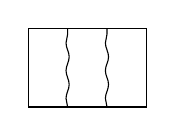
\begin{tikzpicture}[scale=.5]
   \draw (0,0) rectangle (3,2);
   \draw[decorate, decoration={snake, amplitude= .2 mm}] (1,0) -- (1,2);
   \draw[decorate, decoration={snake, amplitude= .2 mm}] (2,0) -- (2,2);        
      \end{tikzpicture}
    \end{center}
  \item  Não se espera que, nesta atividade, os alunos usem a medida para fazer a equipartição de maneira precisa.
    \item Busque conduzir a discussão nos grupos de modo que os estudantes percebam que, para que os amigos recebam a mesma quantidade de chocolate, a partição proposta para a barra de chocolate deve ser em ``partes iguais'', no sentido de ganharem todos a mesma quantidade de chocolate, não necessariamente pedaços de mesma forma.
    \item Na discussão, procure destacar que a referência à ``partição em três partes iguais'' se dá a partir das expressões ``um terço'' da barra de chocolate ou ``a terça parte'' da barra de chocolate.
    \item O item c) admite diversas soluções, algumas estão apresentadas como resposta. No entanto, algumas dessas respostas podem não aparecer naturalmente em sala de aula. Avalie a possibilidade de apresentar e explorar algumas dessas soluções (ou outras que queira) em sala de aula. Por exemplo, apresente uma dessas divisões aos alunos e peça-lhes que avaliem a equipartição, explicando sua decisão.
    \item O item d), provavelmente, pode não ser respondido corretamente pelos alunos. Se for o caso, as expressões ``um terço de'' e ``a terça parte de'' devem ser apresentadas.
    \item Fique atento às falas dos alunos. Observe que os alunos podem representar e verbalizar as respostas de diferentes modos e que não há uma resposta única para a atividade. Por exemplo, alguns alunos podem precisar de mais tempo do que outros para usar a expressão       ``um terço'' no lugar de       ``partição em três partes iguais'' ou ``divisão em três partes iguais''. Ou ainda, observarem que há diferentes representações para a equipartição.
      \item Pode ser aproveitada a oportunidade para questionar os estudantes se no lugar de três amigos fossem 5 amigos, cada um receberia mais ou menos chocolate após a divisão em cinco partes iguais? 
\end{itemize} %s


\begin{itemize} %s
    \item Esta atividade pode ser adaptada visando a inclusão de alunos com deficiência de visão. Para isso, sugere-se confeccionar os modelos da barra de chocolate  inteira e repartida, que estão disponíveis para reprodução no final do livro, em três materiais diferentes. Por exemplo, papel comum e papéis com texturas diferentes, tecido ou material emborrachado.
\end{itemize} %s
\end{orientacoes}
%\vfill
\begin{solucao}{}{}
  \begin{enumerate}[a),wide,labelindent=0pt] %s
    \item       Este item não possui resposta correta, apenas respostas coerentes com a explicação do aluno. Por exemplo, um estudante pode dizer que sim e explicar que o amigo mais velho deve ficar com uma parte maior porque precisa de mais energia. Mas a resposta esperada é que a divisão não parece justa porque as quantidades de chocolate são diferentes. Discuta com os alunos para que entendam a divisão correspondente à resposta esperada.
    \item Não, eles receberão quantidades diferentes de chocolate, embora cada um receba um único pedaço do chocolate.
    \item Respostas possíveis:

  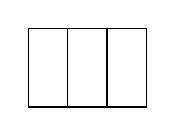
\begin{tikzpicture}[scale=.5]
   \draw (0,0) rectangle (3,2);
   \draw (1,0) -- (1,2);
   \draw (2,0) -- (2,2);
  \end{tikzpicture}
  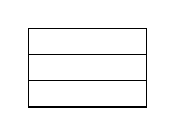
\begin{tikzpicture}[scale=.5]
   \draw (0,0) rectangle (3,2);
   \draw (0,.6666) -- (3,.6666);
   \draw (0,1.3333) -- (3,1.3333);
  \end{tikzpicture}
  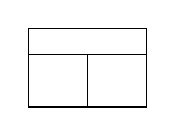
\begin{tikzpicture}[scale=.5]
   \draw (0,0) rectangle (3,2);
   \draw (0,1.3333) -- (3,1.3333);
   \draw (1.5,0) -- (1.5,1.333);
  \end{tikzpicture}
  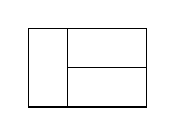
\begin{tikzpicture}[scale=.5]
   \draw (0,0) rectangle (3,2);
   \draw (1,0) -- (1,2);
   \draw (1,1) -- (3,1);
  \end{tikzpicture}

  %\noindent\includegraphics[width=.45\textwidth, keepaspectratio]{../..//media/cap1/secoes/licao1_atv1.png}
    \item       Cada parte é {\it um terço} da barra ou a {\it terça parte} da barra.
\end{enumerate} %s
\end{solucao}

%\subsection{Atividade 2}

\begin{objetivos}{}{}
\begin{itemize} %s
    \item       Perceber que uma unidade (no caso, uma pizza) pode ser subdividida em um mesmo número de partes sem que cada divisão represente uma equipartição.
    \item       Distinguir uma equipartição dentre partições diversas.
    \item       Diferenciar       ``a divisão da unidade em quatro partes quaisquer'' da       ``divisão da unidade em quatro partes iguais''.
    \item       Compreender as expressões ``um quarto de'' e ``quarta parte de'' como forma de identificar uma das partes da equipartição em 4 partes.
\end{itemize} %s
\end{objetivos}

\begin{orientacoes}
  \begin{itemize} %s
    \item No final deste volume estão disponíveis materiais para reprodução.
    \item Recomenda-se que a atividade seja desenvolvida em grupos de 3 a 5 alunos.
    \item As diversas soluções apresentadas pelos diferentes grupos devem ser discutidas com a turma inteira.
    \item É importante que a discussão conduza os alunos ao entendimento de que apenas as partes da equipartição podem ser chamadas de ``quartos'' da pizza, as demais são simplesmente fatias ou pedaços, por exemplo.
    \item Os alunos devem reconhecer que, apesar de todas as pizzas estarem repartidas em quatro fatias, apenas uma das repartições propostas sugere a equipartição, respondendo assim a último item desta atividade.
    \item       Essa atividade pode ser adaptada visando à inclusão de alunos com deficiência visual. Para isso, sugere-se confeccionar os modelos das três pizzas repartidas, que estão disponíveis para reprodução no final do livro, em três materiais diferentes. Por exemplo, papel comum e papéis com texturas diferentes, tecido ou material emborrachado.
\end{itemize} %s
\end{orientacoes}

\begin{solucao}{}{}
\begin{enumerate} [a),wide,labelindent=0pt] %d
    \item       Sim. Cada grupo repartiu sua pizza em quatro fatias.
    \item       Não, pois algumas fatias têm quantidades de pizza diferentes das outras.
    \item       Apenas no grupo 1 as 4 crianças receberam a mesma quantidade de pizza. Cada fatia da pizza do grupo 1 é {\it um quarto} da pizza ou {\it a quarta parte} da pizza.
\end{enumerate} %d
\end{solucao}



\begin{objetivos}{}{}
\begin{itemize} %s
    \item       Reconhecer a equipartição em um modelo linear.
    \item       Reconhecer a quarta parte como a metade da metade.
\end{itemize} %s
\end{objetivos}

\begin{orientacoes}
\begin{itemize} %s
   \item No final deste volume estão disponíveis materiais para reprodução. Esta atividade necessita deste material.
   \item Recomenda-se que esta atividade seja desenvolvida em grupos de quatro alunos.
   \item       Cada grupo deve receber um pedaço de barbante de, aproximadamente, 1m e quatro enfeites (todos iguais).
    \item       Os quatro enfeites precisam ser confeccionados antes da realização da tarefa. Sugerem-se estrelas, cujos modelos estão disponíveis para reprodução no final do livro. No entanto, segundo a avaliação do professor, os enfeites podem ser outros, desde que sejam os 4 congruentes.
    \item       Como sugestão, se possível, solicitar aos alunos que confeccionem os enfeites, por exemplo, associando esta atividade com geometria, com a abordagem de grandezas e medidas, com a disciplina de artes ou envolvendo culturas artesanais populares.
    \item       A equipartição do barbante não deve ser obtida a partir da medida do barbante, mas por sucessivas dobras do barbante sobre ele mesmo, como ilustrado na resposta da atividade. Tal discussão também  será útil na abordagem de frações equivalentes na Lição 4.
    \item       A manipulação e a dobra do barbante devem sustentar a discussão para a identificação da       ``metade da metade'' com a       ``quarta parte'' do barbante. Nesse caso, a identificação se dará pela sobreposição das partes.
      \item Nossa experiência aplicando esta atividade tem mostrado um efeito emocional positivo em permitir que os estudantes realmente confeccionem os enfeites.
\end{itemize} %s

%\vspace*{\fill}
%\columnbreak
\end{orientacoes}

\begin{solucao}{}{}
Uma maneira de se cortar o barbante é dobrar ao meio e depois dobrar novamente ao meio, obtendo quatro partes iguais, como ilustrado na figura a seguir.
  \begin{center}
  \includegraphics[width=200pt, keepaspectratio]{../figuras/licao01/ativ3_fig03.png}
  \end{center}
\end{solucao}
\end{multicols}

\subsection{Sobre o Organizando as Ideias}

  Nesta etapa, espera-se que os alunos compreendam as frações como forma de expressar quantidades. O objetivo é que percebam seu papel para expressar quantidades em situações de equipartição da unidade. Assim, as frações podem ser utilizadas no dia a dia para identificar quantidades do mesmo modo que os números naturais, já conhecidos dos alunos. Por exemplo, como nas expressões:   ``dois ovos'',   ``duas xícaras de farinha'',   ``um terço de xícara de cacau'' e   ``meio litro de leite''.

  Objetiva-se a expressão verbal e não a representação simbólica. Espera-se, assim, que os alunos apropriem-se das expressões verbais que identificam as frações unitárias (um meio, um terço, um quarto, ... , um nono e um décimo) antes de serem apresentados formalmente à simbologia matemática (que será objetivo da próxima lição).  A referência às frações unitárias com a expressão   ``um'' antes da identificação da parte, como, por exemplo, em   ``um terço'' e em   ``um sétimo'', é uma decisão pedagógica. Claro que é possível referir-se a essas frações simplesmente por   ``terço'' e   ``sétimo'', respectivamente. No entanto, nas próximas seções, pretende-se que as frações não unitárias, como   ``dois terços'' e ``nove sétimos'', por exemplo, sejam entendidas a partir da justaposição das frações unitárias correspondentes, o que é naturalmente amparado pela contagem. Nas expressões verbais relativas às frações unitárias, o   ``um'' antes da identificação da parte está associado à contagem. Dessa forma, a compreensão das frações   ``um terço'' e   ``dois terços'' ou das frações ``um sétimo'' e ``nove sétimos'', por exemplo, seguem a mesma construção lógica.

\Bg

\begin{multicols}{2}
\begin{objetivos}{}{}
  \begin{itemize} %s
    \item       Reconhecer que, em uma equipartição, as partes podem não ter a mesma forma.
    \item       Identificar a equivalência entre as partes de uma equipartição a partir de sobreposição ou da comparação pelo reconhecimento da associação a uma mesma fração unitária (no caso,um quarto).
    \item       Reconhecer a quarta parte como a metade da metade.
\end{itemize} %s
\end{objetivos}

\begin{orientacoes}
  \begin{itemize} %s
    \item No final deste volume estão disponíveis materiais para reprodução.
    \item Recomenda-se que esta atividade seja desenvolvida em grupos de 3 a 5 alunos.
    \item Cada estudante deve receber os oito retângulos coloridos, disponíveis para reprodução no final do livro.
    \item Caso não seja possível imprimir os retângulos em cores, use a versão em preto e branco, também disponível no final do livro, e peça para os estudantes colorirem. O objetivo das cores é facilitar a identificação dos retângulos na discussão em sala.
    \item É importante observar que todos os retângulos estão divididos em quartos. Conduza a discussão de modo a levar os alunos a reconhecer que, em uma equipartição, as partes não precisam ter a mesma forma.
    \item Nesta atividade, espera-se que os alunos consigam lidar com a figura de um retângulo como representativa de uma unidade genérica.  No entanto, se necessário, o professor pode associar cada retângulo a um objeto concreto (por exemplo, uma barra de chocolate ou a um pedaço de bolo).
    \item É esperado que não seja imediato o reconhecimento de que as partes dos retângulos da segunda linha representam quartos. Nesse caso,  uma alternativa possível é solicitar que eles recortem as partes de cada um dos retângulos da primeira linha para realizar a comparação por sobreposição com as partes dos retângulos da segunda linha.
   \item Recomenda-se ressaltar para os estudantes ao término da atividade que um quarto é a metade da metade.
    \item Em alguns casos, a comparação se dará pela identificação da fração unitária correspondente a cada parte. Nesses casos, o aluno deve reconhecer que a quarta parte é equivalente à metade da metade. Por exemplo, como no caso seguir.
 
\end{itemize} %s

\noindent 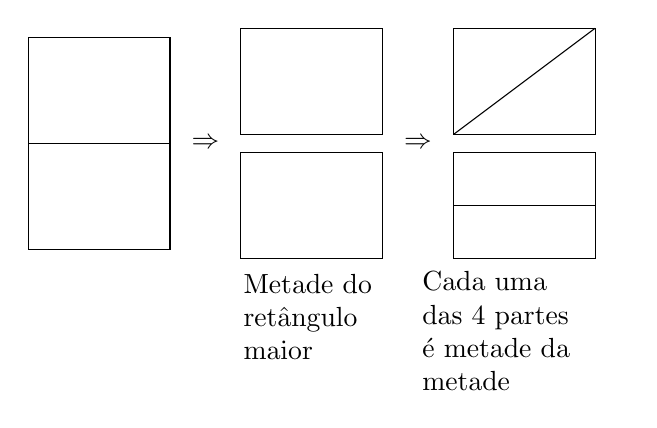
\begin{tikzpicture}[scale=0.45]
  \draw (0,0) rectangle (4,3);
  \draw (0,3) rectangle (4,6);
 % \draw (0,1.5) -- (4,1.5);
  \draw (5,3) node{$\Rightarrow$};
  \draw (6,-0.25) rectangle (10,2.75);
  \draw (6,3.25) rectangle (10,6.25);
  \node[text width=2cm]  at (8.3,-1.9) {Metade do retângulo maior};
  \draw (11,3) node{$\Rightarrow$};
  \draw (12,-0.25) rectangle (16,2.75);
  \draw (12,3.25) rectangle (16,6.25);
  \draw (12,3.25) -- (16,6.25);
  \draw (12,1.25) -- (16,1.25);
  \node[text width=2.5cm]  at (13.9,-2.3) {Cada uma das 4 partes é metade da metade};
  \end{tikzpicture}
\begin{itemize} %s
\item Segundo a avaliação do professor, a atividade pode ser realizada em duas etapas. Em um primeiro momento, os alunos recebem as primeiras quatro das oito imagens e realizam a atividade com essas imagens - cuja comparação se dá apenas pela sobreposição. Em seguida, recebem as outras quatro, para concluir a atividade. 

\item Da experiência dos autores com a implementação desta atividade em sala de aula, constatou-se uma empolgação dos estudantes quando, ao percebem que formas diferentes podem representar a mesma fração da unidade, foram convidados a gerarem outras equipartições dessa unidade. Seguem outras possíveis equipartições:

  \begin{center}
    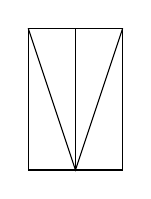
\begin{tikzpicture}[scale=.3]
      \draw[black] (0,0) rectangle (4,6);
      \draw (2,0) -- (2,6);
      \draw (0,6) -- (2,0) -- (4,6);
    \end{tikzpicture}\quad\quad\quad
        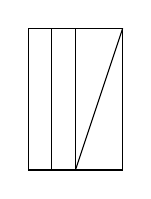
\begin{tikzpicture}[scale=.3]
      \draw[black] (0,0) rectangle (4,6);
      \draw (2,0) -- (2,6);
      \draw (1,0) -- (1,6);
      \draw (2,0) --  (4,6);
    \end{tikzpicture}\quad\quad\quad
        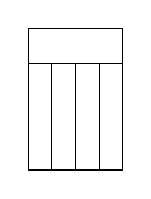
\begin{tikzpicture}[scale=.3]
      \draw[black] (0,0) rectangle (4,6);
      \draw (1,0) -- (1,4.5);
      \draw (2,0) -- (2,4.5);
      \draw (3,0) -- (3,4.5);
      \draw (0,4.5) --  (4,4.5);
    \end{tikzpicture}
  \end{center}
\end{itemize} %s
\end{orientacoes}

\begin{solucao}{}{}
\begin{enumerate}[a),wide,labelindent=0pt] %s
    \item       Todos os retângulos estão divididos em quartos.
    \item       Dois desenhos possíveis são:
\begin{center}
    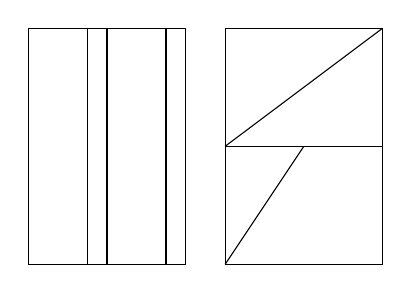
\begin{tikzpicture}[scale=5, x=1mm, y=1mm]
  \draw (0,0) rectangle (1.5,6);
  \draw (1.5,0) rectangle (2,6);
  \draw (2,0) rectangle (3.5,6);
  \draw (3.5,0) rectangle (4,6);
  \draw (5,0) rectangle (9,3);
  \draw (5,3) rectangle (9,6);
  \draw (5,0) -- (7,3);
  \draw (5,3) -- (9,6);
\end{tikzpicture}
\end{center}
\end{enumerate} %s
\end{solucao}

\end{multicols}
\begin{objetivos}{}{}
\begin{itemize} %s
    \item       Identificar uma mesma fração unitária (no caso, a terça parte) em representações diversas.
\end{itemize} %s
\end{objetivos}

\begin{orientacoes}

\begin{itemize} %s
    \item       Recomenda-se que esta atividade seja desenvolvida em grupos de 3 a 5 alunos.
    \item       Durante a discussão, os alunos devem ser estimulados a explicar as suas escolhas. A discussão sobre os motivos da identificação, ou não, de cada uma das representações à terça parte da unidade correspondente será fundamental para atingir o objetivo da atividade.
    \item       Os alunos devem reconhecer que, seja qual for a unidade considerada, em uma equipartição em 3 partes, cada uma das partes é um terço (ou a terça parte) da unidade.
    \item       Aproveite as próprias palavras e os argumentos dos alunos para conduzi-los às conclusões esperadas.
    \item       Fique atento aos alunos que selecionarem as figuras que simplesmente possuem alguma associação com o número 3, não correspondendo a terços. Por exemplo, um aluno que associe a       {\bf Figura i)} a terços pode ainda não ter compreendido a necessidade da equipartição para a identificação de um terço. Já o aluno que associa       {\bf Figura j)}       a terços pode estar simplesmente contando as partes em vermelho, sem que tenha reconhecido que a figura deveria estar dividida em 3 partes iguais e não em 5.
\end{itemize} %s
\end{orientacoes}

\begin{solucao}{}{}
A parte em vermelho representa um terço da figura nos itens b), c), e), h) e j).
\end{solucao}
\pagebreak

\begin{objetivos}{}{}
  \begin{itemize} %d
    \item       Recompor a unidade a partir de uma fração unitária dada em modelos contínuos.
    \item       Relacionar uma fração da unidade à quantidade necessária dessas partes para compor a unidade. Assim, por exemplo, é necessário reunir cinco       {\it quintas partes}       para recompor a unidade.
\end{itemize} %d
\end{objetivos}

\begin{orientacoes}
  \begin{itemize} %d
  \item Recomenda-se que a atividade seja desenvolvida em grupos de 3 a 5 alunos.
    \item No final deste volume estão disponíveis materiais para
reprodução para esta atividade.
    \item É importante ter em mente que existem várias soluções para cada item. Por exemplo, o primeiro item pode ser corretamente respondido por:             \begin{tikzpicture}[scale=.2]
\draw [fill=common, fill opacity=.3] (0,0) arc (0:180:3) -- (0,0) -- cycle;
\draw (-3,0) -- (-3,3);
\end{tikzpicture}
 e
 \begin{tikzpicture}[scale=.2]
\draw [fill=common, fill opacity=.3] (0,0) arc (0:90:3) -- (-3,0) -- cycle;
\draw [fill=common, fill opacity=.3] (-3,0) arc (270:180:3) -- (-3,3) -- cycle;
\end{tikzpicture}.
    \item       Avalie a possibilidade de discutir com os estudantes respostas que sejam reuniões de partes não justapostas, por exemplo, no primeiro item pode-se ter também             \begin{tikzpicture}[scale=.2]
\draw [fill=common, fill opacity=.3] (0,0) arc (0:90:3) -- (-3,0) -- cycle;
\draw [fill=common, fill opacity=.3] (3.7,0) arc (0:90:3) -- (0.7,0) -- cycle;
\end{tikzpicture}
      como resposta.
    \item Estimule os alunos a reconhecer (e a fazer) mais do que uma representação para a unidade em cada item.
    \item Estimule os alunos a, a partir da identificação da fração unitária, determinar a quantidade de partes necessárias para recompor a unidade.
\end{itemize} %d
\end{orientacoes}

\begin{solucao}{}{}
Algumas possibilidades de respostas para cada linha da tabela do enunciado estão nas respectivas linhas abaixo.
\begin{center}


  
% arcos de círculos
 \def \sc {0.22}
 \def\h{1.8}
 
  \begin{longtable}{|m{0.2\linewidth}|m{0.3\linewidth}|m{0.4\linewidth}|}
  \hline
\centering Fração da unidade & \centering Nome da fração da unidade  & \quad\quad\quad Unidade  \\
\hline \hline
\endhead
\centering \begin{tikzpicture}[scale=\sc]
 \draw [fill=common, fill opacity=.3] (0,0) arc (0:90:3) -- (-3,0) -- cycle;
\end{tikzpicture}
&\centering \parbox[c][\h cm][c]{0.01cm}{  } metade  & \begin{tikzpicture}[scale=\sc]
\draw [fill=common, fill opacity=.3] (0,0) arc (0:180:3) -- (0,0) -- cycle;
\draw (-3,0) -- (-3,3);
\end{tikzpicture}
\quad
\begin{tikzpicture}[scale=\sc]
\draw [fill=common, fill opacity=.3] (0,0) arc (0:90:3) -- (-3,0) -- cycle;
\draw [fill=common, fill opacity=.3] (-3,0) arc (270:180:3) -- (-3,3) -- cycle;
\end{tikzpicture}
  \\
    \hline
\centering\begin{tikzpicture}[scale=\sc]
\draw [fill=common, fill opacity=.3] (0,0) arc (0:90:3) -- (-3,0) -- cycle;
\end{tikzpicture}        &\parbox[c][\h cm][c]{0.01cm}{  } \centering   um terço  & \begin{tikzpicture}[scale=\sc]
\draw [fill=common, fill opacity=.3] (0,0) arc (0:270:3) -- (-3,0) -- cycle;
\draw (-3,0) -- (-6,0);
\draw (-3,0) -- (-3,3);
\end{tikzpicture}
\quad
\begin{tikzpicture}[scale=\sc]
\draw [fill=common, fill opacity=.3] (0,0) arc (0:90:3) -- (-3,0) -- cycle;
\draw [fill=common, fill opacity=.3] (-3,0) arc (270:180:3) -- (-3,3) -- cycle;
\draw [fill=common, fill opacity=.3] (-3,0) arc (180:270:3) -- (0,0) -- cycle;
\end{tikzpicture}
 \\
    \hline
\centering \begin{tikzpicture}[scale=\sc]
\draw [fill=common, fill opacity=.3] (0,0) arc (0:90:3) -- (-3,0) -- cycle;
\end{tikzpicture}        & \centering \parbox[c][\h cm][c]{0.01cm}{  } um quarto  & \begin{tikzpicture}[scale=\sc]
\draw [fill=common, fill opacity=.3] (0,0) arc (0:360:3) -- (-3,0) -- cycle;
\draw (-3,0) -- (-6,0);
\draw (-3,0) -- (-3,3);
\draw (-3,0) -- (-3,-3);
\end{tikzpicture}
\quad
\begin{tikzpicture}[scale=\sc]
\draw [fill=common, fill opacity=.3] (0,3) arc (90:270:3) -- (0,3) -- cycle;
 \draw [fill=common, fill opacity=.3] (3,3) arc (0:-90:3) -- (0,3) -- cycle;
 \draw [fill=common, fill opacity=.3] (0,0) arc (90:0:3) -- (0,-3) -- cycle;
 \draw  (0,0) -- (-3,0);
\end{tikzpicture}
 \\
    \hline
\centering \begin{tikzpicture}[scale=\sc]
\draw [fill=common, fill opacity=.3] (0,0) rectangle (3,3);
\end{tikzpicture}
  & \centering \parbox[c][\h cm][c]{0.01cm}{  } metade  & \begin{tikzpicture}[scale=\sc]
\draw [fill=common, fill opacity=.3] (0,0) rectangle (3,3);
\draw [fill=common, fill opacity=.3] (3,0) rectangle (6,3);
\end{tikzpicture}
\quad
\begin{tikzpicture}[scale=\sc]
\draw [fill=common, fill opacity=.3] (0,0) rectangle (3,3);
\draw [fill=common, fill opacity=.3] (0,3) rectangle (3,6);
\end{tikzpicture}
 \\
    \hline
\centering \begin{tikzpicture}[scale=\sc]
\draw [fill=common, fill opacity=.3] (0,0) rectangle (3,3);
\end{tikzpicture}
& \centering \parbox[c][\h cm][c]{0.01cm}{  } um terço  &
\begin{tikzpicture}[scale=\sc]
\draw [fill=common, fill opacity=.3] (0,0) rectangle (3,3);
\draw [fill=common, fill opacity=.3] (3,0) rectangle (6,3);
\draw [fill=common, fill opacity=.3] (6,0) rectangle (9,3);
\end{tikzpicture}
 \quad
\begin{tikzpicture}[scale=\sc]
\draw [fill=common, fill opacity=.3] (0,0) rectangle (3,3);
\draw [fill=common, fill opacity=.3] (0,3) rectangle (3,6);
\draw [fill=common, fill opacity=.3] (3,0) rectangle (6,3);
\end{tikzpicture}
 \quad
\begin{tikzpicture}[scale=\sc]
\draw [fill=common, fill opacity=.3] (0,0) rectangle (3,3);
\draw [fill=common, fill opacity=.3] (3,3) rectangle (6,6);
\draw [fill=common, fill opacity=.3] (6,0) rectangle (9,3);
\end{tikzpicture}
\\
    \hline
\centering \begin{tikzpicture}[scale=\sc]
\draw [fill=common, fill opacity=.3] (0,0) rectangle (3,3);
\end{tikzpicture}
& \centering \parbox[c][\h cm][c]{0.01cm}{  } um quarto  &
\begin{tikzpicture}[scale=\sc]
\draw [fill=common, fill opacity=.3] (0,0) rectangle (3,3);
\draw [fill=common, fill opacity=.3] (3,0) rectangle (6,3);
\draw [fill=common, fill opacity=.3] (6,0) rectangle (9,3);
\draw [fill=common, fill opacity=.3] (9,0) rectangle (12,3);
\end{tikzpicture}
\quad
\begin{tikzpicture}[scale=\sc]
\draw [fill=common, fill opacity=.3] (0,0) rectangle (3,3);
\draw [fill=common, fill opacity=.3] (0,3) rectangle (3,6);
\draw [fill=common, fill opacity=.3] (3,0) rectangle (6,3);
\draw [fill=common, fill opacity=.3] (3,3) rectangle (6,6);
\end{tikzpicture}
\quad
\begin{tikzpicture}[scale=\sc]
\draw [fill=common, fill opacity=.3] (0,3) rectangle (3,6);
\draw [fill=common, fill opacity=.3] (0,0) rectangle (3,3);
\draw [fill=common, fill opacity=.3] (3,0) rectangle (6,3);
\draw [fill=common, fill opacity=.3] (6,0) rectangle (9,3);
\end{tikzpicture}
\\
    \hline
\centering \begin{tikzpicture}[scale=\sc]
\draw  (0,0) -- (3,3);
\end{tikzpicture}
& \centering \parbox[c][\h cm][c]{0.01cm}{  } metade  &
\begin{tikzpicture}[scale=\sc]
\draw  (0,0) -- (3,3) -- (6,0);
\end{tikzpicture}
% \begin{tikzpicture}[scale=\sc]
% \draw  (0,0) -- (3,3);
% \draw  (2,0) -- (5,3);
% \end{tikzpicture}
\quad
\begin{tikzpicture}[scale=\sc]
\draw  (0,0) -- (3,3);
\draw  (3,0) -- (0,3);
\end{tikzpicture}
\\
    \hline
\centering \begin{tikzpicture}[scale=\sc]
\draw  (0,0) -- (3,3);
\end{tikzpicture}
& \centering \parbox[c][\h cm][c]{0.01cm}{  } um terço  &
\begin{tikzpicture}[scale=\sc]
\draw  (0,0) -- (3,3) -- (6,0) -- (9,3);
\end{tikzpicture}
% \begin{tikzpicture}[scale=\sc]
% \draw  (0,0) -- (3,3);
% \draw  (2,0) -- (5,3);
% \draw  (4,0) -- (7,3);
% \end{tikzpicture}
 \quad
\begin{tikzpicture}[scale=\sc]
\draw  (0,0) -- (3,3);
\draw  (4,0) -- (1,3);
\draw  (2,0) -- (5,3);
\end{tikzpicture}
\\
    \hline
\centering \begin{tikzpicture}[scale=\sc]
\draw  (0,0) -- (3,3);
\end{tikzpicture}
& \centering \parbox[c][\h cm][c]{0.01cm}{  } um quarto  &
\begin{tikzpicture}[scale=\sc]
\draw  (0,0) -- (3,3) -- (0,6) -- (-3,3) -- (0,0);
\end{tikzpicture}
% \begin{tikzpicture}[scale=\sc]
% \draw  (0,0) -- (3,3);
% \draw  (2,0) -- (5,3);
% \draw  (4,0) -- (7,3);
% \draw  (6,0) -- (9,3);
% \end{tikzpicture}
\quad
\begin{tikzpicture}[scale=\sc]
\draw  (0,0) -- (3,3);
\draw  (4,0) -- (1,3);
\draw  (2,0) -- (5,3);
\draw (2,0) -- (-1,3);
\end{tikzpicture}
\\
\hline
\centering \begin{tikzpicture}[scale=\sc]
\draw [fill=common, fill opacity=.3] (90:2) -- (210:2) -- (330:2) -- cycle;
\end{tikzpicture}  
& \centering \parbox[c][\h cm][c]{0.01cm}{  } metade 
&
\begin{tikzpicture}[scale=\sc]
\draw [fill=common, fill opacity=.3] (90:2) -- (210:2) -- (330:2) -- cycle;
\draw [fill=common, fill opacity=.3, shift={(2*1.732,0)}] (90:2) -- (210:2) -- (330:2) -- cycle;
\end{tikzpicture}
\quad
\begin{tikzpicture}[scale=\sc]
\draw [fill=common, fill opacity=.3] (90:2) -- (210:2) -- (330:2) -- cycle;
\draw [fill=common, fill opacity=.3, rotate around={60:(90:2)}] (90:2) -- (210:2) -- (330:2) -- cycle;
\end{tikzpicture}
\\
    \hline
\centering \begin{tikzpicture}[scale=\sc]
\draw [fill=common, fill opacity=.3] (90:2) -- (210:2) -- (330:2) -- cycle;
\end{tikzpicture}  
& \centering \parbox[c][\h cm][c]{0.01cm}{  } um terço  
&
\begin{tikzpicture}[scale=\sc]
\draw [fill=common, fill opacity=.3] (90:2) -- (210:2) -- (330:2) -- cycle;
\draw [fill=common, fill opacity=.3, shift={(2*1.732,0)}] (90:2) -- (210:2) -- (330:2) -- cycle;
\draw [fill=common, fill opacity=.3, shift={(4*1.732,0)}] (90:2) -- (210:2) -- (330:2) -- cycle;
\end{tikzpicture}
\quad
\begin{tikzpicture}[scale=\sc]
\draw [fill=common, fill opacity=.3] (90:2) -- (210:2) -- (330:2) -- cycle;
\draw [fill=common, fill opacity=.3, shift={(2*1.732,0)}] (90:2) -- (210:2) -- (330:2) -- cycle;
\draw [fill=common, fill opacity=.3, rotate around={120:(330:2)}] (90:2) -- (210:2) -- (330:2) -- cycle;
\end{tikzpicture}
 \quad
\begin{tikzpicture}[scale=\sc]
\draw [fill=common, fill opacity=.3] (90:2) -- (210:2) -- (330:2) -- cycle;
\draw [fill=common, fill opacity=.3, rotate around={60:(90:2)}] (90:2) -- (210:2) -- (330:2) -- cycle;
\draw [fill=common, fill opacity=.3, shift={(2*1.732,0)}] (90:2) -- (210:2) -- (330:2) -- cycle;
\end{tikzpicture}
\\
    \hline
\centering \begin{tikzpicture}[scale=\sc]
\draw [fill=common, fill opacity=.3] (90:2) -- (210:2) -- (330:2) -- cycle;
\end{tikzpicture}  

& \centering \parbox[c][\h cm][c]{0.01cm}{  } um quarto


&
\begin{tikzpicture}[scale=\sc]
\draw [fill=common, fill opacity=.3] (90:2) -- (210:2) -- (330:2) -- cycle;
\draw [fill=common, fill opacity=.3, shift={(2*1.732,0)}] (90:2) -- (210:2) -- (330:2) -- cycle;
\draw [fill=common, fill opacity=.3, shift={(4*1.732,0)}] (90:2) -- (210:2) -- (330:2) -- cycle;
\draw [fill=common, fill opacity=.3, shift={(6*1.732,0)}] (90:2) -- (210:2) -- (330:2) -- cycle;
\end{tikzpicture}
\quad
\begin{tikzpicture}[scale=\sc]
\draw [fill=common, fill opacity=.3] (90:2) -- (210:2) -- (330:2) -- cycle;
\draw [fill=common, fill opacity=.3, rotate around={60:(90:2)}] (90:2) -- (210:2) -- (330:2) -- cycle;
\draw [fill=common, fill opacity=.3, shift={(1.732,3)}] (90:2) -- (210:2) -- (330:2) -- cycle;
\draw [fill=common, fill opacity=.3, shift={(1.732,3)}, rotate around={60:(90:2)}] (90:2) -- (210:2) -- (330:2) -- cycle;
\end{tikzpicture}
\quad
\begin{tikzpicture}[scale=\sc]
\draw [fill=common, fill opacity=.3] (90:2) -- (210:2) -- (330:2) -- cycle;
\draw [fill=common, fill opacity=.3, rotate around={60:(90:2)}] (90:2) -- (210:2) -- (330:2) -- cycle;
\draw [fill=common, fill opacity=.3, rotate around={120:(90:2)}] (90:2) -- (210:2) -- (330:2) -- cycle;
\draw [fill=common, fill opacity=.3, shift={(2*1.732,0)}] (90:2) -- (210:2) -- (330:2) -- cycle;
\end{tikzpicture}
\\
\hline
\end{longtable}
\end{center}
\end{solucao}


\begin{multicols}{2}

  \begin{objetivos}{}{}
\begin{itemize} %s
    \item       Representar uma fração unitária a partir de uma unidade dada.
    \item       Reconhecer (e obter) um quarto como a metade da metade e um oitavo como a metade de um quarto.
    \item       Comparar as frações unitárias metade, um quarto e um oitavo de um mesmo quadrado.
\end{itemize} %s
\end{objetivos}

\begin{orientacoes}
  \begin{itemize} %s
    \item       Esta é uma atividade que o aluno pode fazer individualmente.
    \item       Não se espera que, nesta atividade, os alunos usem a medida para fazer a equipartição de maneira mais precisa. O objetivo é fazer a equipartição livremente e de forma coerente. Assim, por exemplo, podem ser aceitas como respostas:
\end{itemize} %s
\begin{center}
\begin{tikzpicture}[scale=.7]
 \draw[fill=common, fill opacity=.3] (0,0) rectangle (3,3);
 \draw[decorate, decoration={snake, amplitude= .2 mm}] (1.5,0) -- (1.5,3);
\end{tikzpicture}
e
\begin{tikzpicture}[scale=.7]
 \draw[fill=common, fill opacity=.3] (0,0) rectangle (3,3);
 \draw[decorate, decoration={snake, amplitude= .2 mm}] (0,0) -- (3,3);
\end{tikzpicture}
\end{center}
  Já as representações a seguir sugerem que os alunos precisam revisar os conceitos exigidos para a solução da atividade:
\begin{center}
  \begin{tikzpicture}[scale=.7]
 \draw[fill=common, fill opacity=.3] (0,0) rectangle (3,3);
 \draw[decorate, decoration={snake, amplitude= .2 mm}] (2.3,0) -- (2.3,3);
\end{tikzpicture}
\end{center}
\begin{itemize} %s
    \item       A representação da unidade se dá de forma genérica por um quadrado.
    \item       Espera-se que os alunos reconheçam que, para obter um quarto da unidade, basta tomar a metade da metade. E que, para determinar um oitavo, pode-se dividir um quarto ao meio.
    \item       Recomenda-se que os alunos tenham em mãos três quadrados de papel iguais e que sejam orientados a fazer uso de dobradura para identificar as frações pedidas. Assim, por exemplo, a fração um quarto pode ser obtida por duas dobras do papel.
    \item Discuta com os estudantes que, quanto maior o número de partes iguais em que se particiona o quadrado, menor fica cada uma das partes.
    \item Procure apresentar e discutir com a turma mais do que uma solução para cada item.
    \item \textbf{As diferentes soluções apresentadas pelos alunos podem enriquecer a discussão}. A comparação entre, por exemplo, a metade do quadrado proveniente da dobradura pela diagonal e o quarto do quadrado proveniente da dobradura a partir de linhas paralelas aos lados (como um sinal de ``$+$'') pode não ser tão natural. Dificuldade semelhante pode ser observada na comparação entre esse mesmo quarto do quadrado e o oitavo do quadrado proveniente de uma sequência de dobraduras paralelas a um dos lados, determinando ``faixas paralelas''. Nesses casos, para executar a comparação, é necessário que os alunos reconheçam partes de formatos diferentes que correspondem a uma mesma fração do quadrado como iguais em quantidade (no caso, área). Assim, a comparação entre a metade do quadrado, obtida pela dobradura na diagonal, e o quarto do quadrado, obtido pela dobradura ``em sinal de $+$'', pode ser amparada pelo reconhecimento de que a metade em questão é igual em quantidade (área) à metade do quadrado obtida por uma única dobra paralela a um dos lados, que é o dobro do quarto do quadrado.

\begin{center}
  \begin{tikzpicture}[scale=.5]
         \draw[fill=common, fill opacity=.3] (0,0) rectangle (2,2);
         \draw[fill=attention] (0,1) rectangle (2,2);
        \end{tikzpicture}\quad\quad
        \begin{tikzpicture}[scale=.5]
         \draw[fill=common, fill opacity=.3] (0,0) rectangle (2,2);
         \draw[fill=attention] (0,0) -- (2,2) -- (0,2)--cycle;
        \end{tikzpicture}
\end{center}

\item Nossa experiência na implementação desta atividade com estudantes do $6^\circ$ ano mostrou que após os alunos entenderem que se espera mesma quantidade e não mesmo formato, passaram a se divertir indo ao quadro para exibir equipartições diferentes daquelas já exibidas pelos colegas.
\end{itemize} %s
\end{orientacoes}

\begin{solucao}{}{}
  Algumas soluções possíveis, convencionais e outras menos convencionais são:

        \begin{enumerate}[a)]
         \item Metade:   \newline
        \begin{tikzpicture}[scale=.8]
         \draw[fill=common, fill opacity=.3] (0,0) rectangle (2,2);
         \draw[fill=attention] (0,1) rectangle (2,2);
        \end{tikzpicture}
        \begin{tikzpicture}[scale=.8]
         \draw[fill=common, fill opacity=.3] (0,0) rectangle (2,2);
         \draw[fill=attention] (0,0) -- (2,2) -- (0,2)--cycle;
        \end{tikzpicture}
        \begin{tikzpicture}[scale=.8]
         \draw[fill=common, fill opacity=.3] (0,0) rectangle (2,2);
         \draw[fill=attention] (0,2) -- (2,2) -- (1,1)--cycle;
         \draw[fill=attention] (0,0) -- (2,0) -- (1,1)--cycle;
        \end{tikzpicture}
        \begin{tikzpicture}[scale=.8]
         \draw[fill=common, fill opacity=.3] (0,0) rectangle (2,2);
         \draw[fill=attention] (0,1) rectangle (1,2);
         \draw[fill=attention] (1,0) rectangle (2,1);
        \end{tikzpicture}
       \item Um quarto:  \newline
       \begin{tikzpicture}[scale=.8]
         \draw[fill=common, fill opacity=.3] (0,0) rectangle (2,2);
         \draw[fill=attention] (0,0) rectangle (.5,2);
         \foreach \x in {1,1.5} \draw (\x,0) -- (\x,2);
       \end{tikzpicture}
       \begin{tikzpicture}[scale=.8]
         \draw[fill=common, fill opacity=.3] (0,0) rectangle (2,2);
         \draw[fill=attention] (0,1) rectangle (1,2);
         \draw (1,0) -- (1,1);
         \draw (1,1)-- (2,1);
        \end{tikzpicture}
        \begin{tikzpicture}[scale=.8]
         \draw[fill=common, fill opacity=.3] (0,0) rectangle (2,2);
         \draw[fill=attention] (0,0) -- (1,1) -- (0,2)--cycle;
         \draw (1,1) -- (2,2);
         \draw (1,1) -- (2,0);
        \end{tikzpicture}
        \begin{tikzpicture}[scale=.8]
         \draw[fill=common, fill opacity=.3] (0,0) rectangle (2,2);
         \draw[fill=attention] (2,2) -- (1,2) -- (1,1)--cycle;
         \draw[fill=attention] (0,0) -- (1,0) -- (1,1)--cycle;
         \draw (0,2) -- (2,0);
        \end{tikzpicture}
       \item  Um oitavo:  \newline
       \begin{tikzpicture}[scale=.8]
         \draw[fill=common, fill opacity=.3] (0,0) rectangle (2,2);
         \draw[fill=attention] (0,0) rectangle (.25,2);
         \foreach \x in {.5,.75,...,1.75} \draw (\x,0) -- (\x, 2);
       \end{tikzpicture}
       \begin{tikzpicture}[scale=.8]
         \draw[fill=common, fill opacity=.3] (0,0) rectangle (2,2);
         \draw[fill=attention] (0,1) rectangle (.5,2);
         \draw (0,1)--(2,1);
         \foreach \x in {.5,1,...,1.5} \draw (\x,0) -- (\x,2);
        \end{tikzpicture}
        \begin{tikzpicture}[scale=.8]
         \draw[fill=common, fill opacity=.3] (0,0) rectangle (2,2);
         \draw[fill=attention] (0,1) -- (1,1) -- (0,2)--cycle;
         \draw (0,0) -- (1,1);
        \end{tikzpicture}
        \begin{tikzpicture}[scale=.8]
         \draw[fill=common, fill opacity=.3] (0,0) rectangle (2,2);
         \draw[fill=attention] (2,2) -- (1,2) -- (1,1)--cycle;
         \draw (1,1) -- (1,0);
         \draw (0,0) -- (1,1);
         \end{tikzpicture}
       \item  Dentre as opções apresentadas, a maior fração do quadrado é metade.
        \end{enumerate}
\end{solucao}

\begin{objetivos}{}{}
\begin{itemize} %s
    \item       Representar uma fração unitária (no caso, um meio ou metade) a partir de uma unidade não usual dada.
    \item       Estabelecer representações diferentes para a mesma fração unitária de uma mesma unidade.
\end{itemize} %s
 \end{objetivos}

\begin{orientacoes}
\begin{itemize} %s
   \item Esta é uma atividade que o aluno pode fazer individualmente. Mas caso os estudantes tenham dificuldades em encontrar três representações distintas, sugere-se que sejam socializadas suas respostas, quando provavelmente aparecerão mais do que três soluções distintas.
   \item Observe que a representação da unidade se dá de forma genérica, ainda em modelo contínuo, por uma figura não tradicional como retângulos e círculos, que é determinada pela justaposição de dois hexágonos regulares.
   \item       Como na atividade anterior, não se espera que, nesta atividade, o aluno use a medida para fazer a equipartição de maneira mais precisa. O objetivo é que o aluno faça a equipartição livremente e de forma coerente,  mesmo porque aqui não se recomenda o uso de material concreto para a realização da atividade. É esperado que o material concreto utilizado como apoio para as atividades anteriores já seja suficiente para que o estudante abstraia a ideia de equipartição e faça uso de sua imaginação apenas.
   \item Procure apresentar e discutir com a turma mais do que uma solução para cada item.
\end{itemize} %s
\end{orientacoes}

\begin{solucao}{}{}
Algumas das respostas possíveis para este problema são:
\begin{center}
\begin{tikzpicture}[scale=.4]
\draw[fill=attention] (3.,5.) -- (3.,3.) -- (4.7,2.) -- (6.46,3.) -- (6.46,5.) -- (4.73,6.) -- cycle;
\draw[fill=common, fill opacity=.3] (6.46,5.) -- (6.46,3.) -- (8.2,2.) -- (9.9,3.) -- (9.9,5.) -- (8.2,6.) -- cycle;
\end{tikzpicture}\hspace{.2cm}
\begin{tikzpicture}[scale=.4]
\draw[fill=common, fill opacity=.3] (3.,5.) -- (3.,3.) -- (4.7,2.) -- (6.46,3.) -- (6.46,5.) -- (4.73,6.) -- cycle;
\draw[fill=common, fill opacity=.3] (6.46,5.) -- (6.46,3.) -- (8.2,2.) -- (9.9,3.) -- (9.9,5.) -- (8.2,6.) -- cycle;
\draw[fill=attention] (4.732050807568877,6.) -- (3.,5.) -- (3.,3.) -- (4.732050807568877,2.) -- cycle;
\draw[fill=attention] (8.2,6.) -- (8.2,2.) -- (9.9,3.) -- (9.9,5.) -- cycle;
\end{tikzpicture}

\begin{tikzpicture}[scale=.4]
\draw[fill=common, fill opacity=.3] (3.,5.) -- (3.,3.) -- (4.7,2.) -- (6.46,3.) -- (6.46,5.) -- (4.73,6.) -- cycle;
\draw[fill=common, fill opacity=.3] (6.46,5.) -- (6.46,3.) -- (8.2,2.) -- (9.9,3.) -- (9.9,5.) -- (8.2,6.) -- cycle;
\draw[fill=attention] (3.,4.) -- (3.,3.) -- (4.732050807568877,2.) -- (6.464101615137757,3.) -- (8.196152422706634,2.) -- (9.928203230275509,3.) -- (9.928203230275509,4.) -- cycle;
\end{tikzpicture}\hspace{.2cm}
\begin{tikzpicture}[scale=.4]
\draw[fill=common, fill opacity=.3] (3.,5.) -- (3.,3.) -- (4.7,2.) -- (6.46,3.) -- (6.46,5.) -- (4.73,6.) -- cycle;
\draw[fill=common, fill opacity=.3] (6.46,5.) -- (6.46,3.) -- (8.2,2.) -- (9.9,3.) -- (9.9,5.) -- (8.2,6.) -- cycle;
\draw[fill=attention] (3,5) -- (3.,3.) -- (4.73,2.) -- (6.46,3.) -- (8.2,2.) -- (9.9,3.) -- cycle;
\end{tikzpicture}
\end{center}
\end{solucao}
\pagebreak

\begin{objetivos}{}{}
\begin{itemize} %s
    \item       Reconhecer a metade de uma unidade pela reunião de partes menores e em partições diversas.
    \item       Estabelecer representações diferentes para a mesma fração unitária para uma mesma unidade.
\end{itemize} %s
\end{objetivos}

\begin{orientacoes}
  \begin{itemize} %s
  \item       Esta é uma atividade que o aluno pode fazer individualmente.
  \item       Cada aluno deve receber as imagens das figuras, disponíveis para reprodução no final do livro para que possa manipular como achar melhor e conduzir a sua decisão.
  \item       Esta atividade pretende levar o aluno a perceber que a metade de uma unidade pode ser considerada e identificada mesmo sem que se tenha uma divisão em duas partes iguais.
  \item       Como nas atividades anteriores, não se espera que o aluno use a medida para confirmar a metade da unidade. O objetivo é que o aluno identifique a representação da metade (ou não) por sobreposição e justaposição das partes, decompondo e recompondo a figura.
  \item       Incentive os alunos a argumentar, justificando a sua decisão. Para isso, podem, por exemplo, se apoiar em dobraduras ou em recortes das partes da figura.
  \item       Procure apresentar e discutir com a turma mais do que uma solução para cada item.
\end{itemize} %s
\end{orientacoes}

\begin{solucao}{}{}
  As figuras que correspondem à metade da unidade são as de números 1, 2, 4, 5, 6, 8, 9, 11 e 12.
\end{solucao}

\begin{objetivos}{}{}
\begin{itemize}
 \item Distinguir e nomear frações unitárias a partir de suas representações em modelos circulares.
\item  Comparar frações unitárias a partir de suas representações em modelos circulares.
\end{itemize}
\end{objetivos}

\begin{orientacoes}
\begin{itemize}
\item    Esta atividade é planejada para ser desenvolvida a partir de material concreto baseado em modelos circulares. Mais especificamente com um material conhecido como ``Círculos de Frações''. Para aplicá-la, é necessário reproduzir esse material, que está disponível nas páginas para reprodução.
\item Sendo um material concreto, os círculos de frações têm o papel de auxiliar na visualização da representação das frações, mais especificamente, das frações unitárias.
\item Recomenda-se que esta atividade seja desenvolvida em grupos de 3 a 5 alunos. No entanto, cada aluno deve ter o seu próprio material (Círculos de Frações) para realizar a atividade.
\item Durante a discussão, os alunos devem ser estimulados a explicar as suas escolhas. O uso de cores vai fazer parte da comunicação, no entanto a justificativa e raciocínio devem estar apoiados no conceito de fração. %A discussão sobre os motivos da identificação, ou não, de cada uma das representações às frações da unidade correspondentes será fundamental para atingir o objetivo da atividade.
 \item Na versão utilizada nesta atividade, o círculo corresponde à unidade, ou seja, ao 1 e os setores circulares, diferenciados por cores, correspondem às frações unitárias um meio, um terço, um quarto, um sexto, um sétimo, um oitavo, um nono e um décimo.
    \item Refira-se ao círculo na cor preta como círculo ou unidade, e não como todo ou inteiro. Refira-se a cada setor circular como fração do círculo, parte do círculo ou, simplesmente, peça da cor x.
    \item Antes de solicitar aos alunos que realizem a atividade, explore o material ressaltando especialmente o fato de que, reunidas, as peças de uma mesma cor determinam um círculo congruente ao preto.
    \item Ainda antes de solicitar aos alunos que realizem a atividade, explore também o material com perguntas dirigidas a toda a turma como as seguintes: ``Quantas peças azuis cobrem o círculo preto?'' ou ``Quantas peças verdes cobrem o círculo preto?'', sugerindo que as peças coloridas podem ser consideradas frações do círculo preto.
    \item Faça uso do material concreto para ilustrar e explicar a resposta de cada item e incentive os seus alunos a fazerem o mesmo.
    \item Espera-se que a explicação para as respostas, nos oito primeiros itens desta questão, seja a partir da contagem dos setores circulares correspondentes às frações envolvidas. Assim, por exemplo, a resposta do item b) pode ser justificada pelo fato de que são necessários 4 partes de círculo na cor vermelha para compor um círculo preto.
    \item Já para os cinco itens que tratam da comparação, espera-se que os alunos identifiquem os setores que representam as frações envolvidas e procedam a comparação pela sobreposição das peças correspondentes. Assim, por exemplo, a resposta do item l) pode ser justificada pela sobreposição das peças das cores verde e amarelo.
    \item Aproveite a correção desses últimos itens para explorar, a partir dos Círculos de Frações, a relação entre a quantidade de peças de cada cor e o tamanho das peças, ou seja, a relação inversa entre a quantidade de partes em que círculo (unidade) está dividido e o tamanho de cada parte.
    \item Os Círculos de Frações podem ser utilizados para trabalhar outros conceitos e assuntos além de frações unitárias, tais como: frações em geral, comparação de frações e operações com frações (adição e subtração). 
    \end{itemize}
\end{orientacoes}
  \end{multicols}


\begin{solucao}{}{}
  % Faltam as justificativas.
\begin{enumerate}[a)]
 \item Uma peça da cor AZUL é igual a um terço do círculo preto.
 \item    Uma peça da cor VERMELHA é igual a um quarto do círculo preto.
 \item    Uma peça da cor AMARELA é igual a um sétimo do círculo preto.
 \item    Uma peça da cor LARANJA é igual a um nono do círculo preto.
 \item    Uma peça da cor roxa é igual a UM SEXTO do círculo preto.
 \item    Uma peça da cor cinza é igual a UM OITAVO do círculo preto.
 \item    Uma peça da cor branca é igual a UM DÉCIMO do círculo preto.
 \item    Uma peça da cor rosa é igual à METADE do círculo preto.
 \item    Um terço do círculo preto é maior do que um sétimo do círculo preto.
 \item    Um nono do círculo preto é menor do que um quarto do círculo preto.
 \item    Um sétimo do círculo preto é menor do que um quinto do círculo preto.
 \item    Um quarto do círculo preto é maior do que um oitavo do círculo preto.
 \item    Um sexto do círculo preto é maior do que um sétimo do círculo preto
\end{enumerate}

\end{solucao}

\begin{objetivos}{}{}
  \begin{itemize} %s
    \item Conhecer e compreender as expressões correspondentes às frações unitárias com denominadores de 5 a 10.
    \item Comparar frações da unidade por meio da representação visual de frações do círculo.
    \item Reconhecer a relação inversa entre o número de partes e o tamanho de cada parte.
\end{itemize} %s
\end{objetivos}

\begin{orientacoes}
\begin{itemize} %s
    \item       Esta atividade pode ser resolvida individualmente, mas é essencial que seja discutida com toda a turma.
    \item       É provável que nem todos os alunos conheçam ou intuam as expressões correspondentes às frações propostas. Nesse caso, cabe ao professor apresentá-las e diferenciá-las.
    \item       Aproveite esta atividade para revisar e discutir o vocabulário que é objetivo nesta seção:       {\it unidade,}             {\it metade,}             {\it um meio,}             {\it um terço,}             {\it terça parte,}             {\it um quarto,}             {\it quarta parte,}             {\it um quinto,}             {\it quinta parte,}             {\it um sexto,}             {\it sexta parte,}             {\it um sétimo,}             {\it sétima parte,}             {\it um oitavo,}             {\it oitava parte,}             {\it um nono,}             {\it nona parte,}             {\it um décimo}       e       {\it décima parte}      .
\end{itemize} %s
\end{orientacoes}

\begin{solucao}{}{}
\begin{enumerate}[a),wide,labelindent=0pt] %s
    \item       A correspondência adequada é:
\begin{enumerate} [\;\; I), labelindent=0pt] %d
        \item           A esta afirmação corresponde à figura G).
        \item           A esta afirmação corresponde à figura D).
        \item           A esta afirmação corresponde à figura I).
        \item           A esta afirmação corresponde à figura B).
        \item           A esta afirmação corresponde à figura A).
        \item           A esta afirmação corresponde à figura F).
\end{enumerate} %d

    \item       As frações um sétimo, um oitavo, um nono e um décimo do círculo são menores que um sexto do círculo. Qualquer uma delas está correta. Portanto qualquer uma delas serve como resposta.
    \item       As frações um meio, um terço, um quarto, um quinto, um sexto, um sétimo e um oitavo do círculo são maiores que um nono do círculo. Qualquer uma delas está correta.
    \item       As frações um sétimo e um oitavo do círculo são menores que um sexto e maiores que um nono do círculo.
\end{enumerate} %s
\end{solucao}

\Bg

\begin{objetivos}{}{}
\begin{itemize} %s
    \item Reconhecer e diferenciar a representação das frações ``um meio'', ``um quarto'' e       ``um décimo'' em modelos diversos, baseados  ou não em equipartição.
\end{itemize} %s
\end{objetivos}

\begin{orientacoes}
\begin{itemize} %s
\item       Esta é uma atividade que o aluno pode fazer individualmente.
\item Esta atividade pode ser desenvolvida com o uso do material para reprodução disponível no final do livro caso se entenda que seus estudantes ainda precisam deste recurso.
\item Como nas atividades anteriores, não se espera que os alunos usem a medida para confirmar a metade. O objetivo é que identifiquem a representação da metade (ou não) por sobreposição e justaposição dessas partes, decompondo e recompondo a figura.
\item No item m), pretende-se que o estudante considere o quadrado maior como unidade e perceba que a parte em vermelho corresponde à metade desse quadrado. Isso pode ser feito observando que todos os quadradinhos vermelhos podem ser agrupados para formar a metade superior do quadrado maior e os azuis agrupados para formar a parte de baixo, por exemplo.
\begin{center}
  \begin{tikzpicture}[scale=.5]
\draw[fill=common, fill opacity=.3] (0,0) rectangle (4,4);
 \filldraw[fill=attention, draw=black] (1,0) rectangle (2,1);
 \filldraw[fill=attention, draw=black] (3,0) rectangle (4,1);
 \filldraw[fill=attention, draw=black] (0,1) rectangle (1,2);
 \filldraw[fill=attention, draw=black] (2,1) rectangle (3,2);
 \filldraw[fill=attention, draw=black] (1,2) rectangle (2,3);
 \filldraw[fill=attention, draw=black] (3,2) rectangle (4,3);
 \filldraw[fill=attention, draw=black] (0,3) rectangle (1,4);
 \filldraw[fill=attention, draw=black] (2,3) rectangle (3,4);
\end{tikzpicture}
\quad
\begin{tikzpicture}[scale=.5]
  \draw[fill=common, fill opacity=.3] (0,0) rectangle (4,4);
  \filldraw[fill=attention, draw=black] (0,2) rectangle (4,4);
  \draw (0,0) grid (4,4);
\end{tikzpicture}
\end{center}

Neste item m), é prematuro e, portanto, inadequado usar o argumento de que a fração é um meio argumentando que dos 16 quadradinhos, existem 8 pintados de vermelho. Isso porque, nessa linha de raciocínio, a unidade seria o quadradinho e não o quadrado maior e, consequentemente, não se estaria fazendo uma divisão de uma unidade mas, sim, uma contagem em um modelo discreto de frações, abordagem essa que escolhemos evitar nesse momento.   


\item Incentive os alunos a argumentar, justificando a sua decisão. Para isso, podem, por exemplo, se apoiar em dobraduras ou no recorte das partes da figura.
\item Procure apresentar e discutir com a turma mais do que uma solução para cada item.
\end{itemize} %s
\end{orientacoes}

\begin{solucao}{}{}
  \begin{tabular}{lll}
a) um meio,&  b) um décimo,& c) um quarto,\\
d) um quarto,& e) um quarto,& f) um meio,\\
g) um quarto,& h) um décimo,& i) um quarto,\\
j) um décimo,& l) um quarto,& m) um meio
\end{tabular}
\end{solucao}

\clearpage
\ifdefined\telas
 \else
 \mbox{}
 \newpage
 \fi
 
\noindent {\color{special}{\Large \bf LIÇÃO 2 - Para o professor}}
\vspace{.5cm}

Na Lição anterior, as frações unitárias permitiram reconhecer e registrar quantidades menores que a unidade: meio, um terço, um quarto, etc. Nesta, serão abordadas as frações em geral: as que representam quantidades menores do que a unidade, quantidades maiores do que a unidade ou quantidades inteiras. Também serão introduzidas a notação simbólica de frações e a comparação entre frações de mesmo denominador. 

As frações com numerador diferente de 1 são apresentadas \textbf{reunindo-se (por contagem ou por justaposição) cópias de uma mesma fração unitária.}
Cabe ressaltar que reunir aqui não tem como objetivo tratar da operação de adição, ou seja, não se espera que o aluno compreenda, nem que seja apresentado a ele, $2/3$ como $1/3 + 1/3$. Espera-se no entanto que o raciocínio aditivo, elementar na contagem, ampare a compreensão do aluno.

Para isso, tem-se a representação pictórica como um apoio importante.
Na Atividade 1, as imagens das pizzas amparam a compreensão das frações três quartos, cinco sextos e cinco oitavos como a reunião de cópias de frações unitárias correspondentes à quarta parte, à sexta parte e à oitava parte de uma pizza, respectivamente. Nesse sentido, nas primeiras atividades, há um esforço deliberado para que o estudante faça uso da linguagem de frações apresentada na Lição 1 para expressar frações não unitárias.
Na Atividade 2, as imagens da barra de chocolate amparam a compreensão da fração dois terços como a reunião de duas partes correspondentes à terça parte (ou à fração um terço) de uma barra de chocolate.
Na Atividade 3, sabendo que uma das cinco fatias iguais em que foi repartida uma torta é um quinto da torta, espera-se que o aluno use a linguagem ``dois quintos'' ou ``dois um quintos'' da torta para se referir às outras duas fatias.
Dessa forma, ``dois quintos'' da torta são obtidos pela reunião de duas partes correspondentes a ``um quinto'' da torta.
O objetivo é que esse processo se estenda para a compreensão das frações não unitárias.
Assim, as frações ``quatro quintos'' e ``seis quintos'' são entendidas como a reunião de ``quatro um quintos'' e ``seis um quintos'' da mesma unidade, respectivamente. O processo de reunir frações unitárias pode ser observado como uma contagem (com justaposição ou não) em que a fração unitária tem o papel de unidade na contagem. A fração unitária é uma subunidade da unidade considerada. 

Um cuidado especial recomendado ao professor é com as frações que representam uma quantidade maior que a unidade, introduzidas logo nas primeiras atividades ainda sem notação simbólica. Não é indicado atrasar muito a introdução deste tipo de fração porque o estudante pode fixar-se na ideia de que não há fração maior do que a unidade  (por exemplo, a fração quatro terços pode não fazer sentido para o estudante porque, para ele, não faz sentido dividir uma torta em 3 pedaços e tomar 4). Decidiu-se omitir as terminologias ``fração própria'', ``fração imprópria'' e ``fração aparente'' por se acreditar que esta linguagem não só é desnecessária para a aprendizagem do assunto como também por poder desviar a atenção dos conceitos que realmente importam.
A representação de frações maiores que a unidade na forma de número misto também não é adotada neste texto. Esse tipo de representação não tem um uso que justifique a abordagem nesta etapa da aprendizagem.

Apesar de esta lição introduzir a linguagem simbólica de frações, o estudante talvez ainda precise de uma unidade concreta explícita para dar um significado para a fração $\frac{a}{b}$: por exemplo, ``$\frac{a}{b}$ de uma pizza'' ou ``$\frac{a}{b}$ de uma barra de chocolate''. Apenas na próxima lição, a fração $\frac{a}{b}$ será tratada como número, requerendo a abstração que o conceito de número exige.
\vspace{.15cm}

\noindent OBJETIVOS ESPECÍFICOS DA LIÇÃO 2:
\vspace{.15cm}

\noindent O aluno deve ser capaz de:
\begin{itemize}
 \item  Reconhecer a necessidade de apresentar uma expressão verbal que identifique a quantidade correspondente à junção de duas ou mais partes correspondentes às frações unitárias de mesmo denominador.
 \item  Reconhecer frações não unitárias como a reunião de cópias de frações unitárias de uma mesma unidade. 
 \item  Utilizar as linguagens verbal e simbólica para referir-se a uma fração $\frac{a}{b}$.
 \item  Reconhecer e nomear os termos de uma fração (numerador e denominador). 
 \item  Comparar frações de mesmo denominador.
 \item Reconhecer o papel da unidade na identificação da fração, tanto em situações em  que uma mesma fração pode representar quantidades diferentes como em situações em que frações diferentes podem representar uma mesma quantidade.
\end{itemize}


\pagebreak

%\begin{multicols}{2}
\begin{objetivos}[code={\setcounter{tcb@cnt@objetivos}{0}}, label=chap2-ativ1]{}{}  %o comando entre colchetes reinicia a numeração dos objetivos manualmente do zero.
  \begin{itemize} %s
\item Estender o conceito de frações para expressar quantidades que correspondam a mais do que uma fração unitária, a partir da junção de duas ou mais partes correspondentes às frações unitárias de mesmo denominador.
\item Reconhecer a necessidade de apresentar uma expressão verbal que identifique a quantidade correspondente à junção de duas ou mais partes correspondentes às frações unitárias de mesmo denominador.
  \end{itemize} %s
\end{objetivos}

\begin{orientacoes}{}{}
  \begin{itemize} %s
\item Recomenda-se que a atividade seja realizada individualmente e que os alunos compartilhem suas respostas. 
\item É possível que os alunos utilizem expressões variadas para nomear as quantidades de pizza que cada amigo comeu. Por exemplo, ``três de quatro fatias'', ``três fatias de um quarto de pizza'', ``três quartos de pizza'', dentre outras. É importante que a discussão conduza os alunos ao uso de quartos, sextos e oitavos: ``três quartos'', ``cinco sextos'', ``cinco oitavos'', etc. 
\end{itemize} %s
\end{orientacoes}
%  \noindent {\bf Classificações:}\vspace{.1cm}
% \begin{itemize} %s
%     \item       Heid et al.: Conceito: identificar e descrever
%     \item       Nicely, Jr.: Nível 1: reconhecer
%     \item       UERJ: Observar: identificar e reconhecer
% \end{itemize} %s

\begin{solucao}[code={\setcounter{tcb@cnt@solucao}{0}}]{}{}
  \label{ativ:sobra-de-pizza}
\begin{enumerate} [\quad a)] %d
\item Da esquerda para a direita as pizzas são de João, Mariele e Luiza.
\item Na pizza de João uma fatia representa um sexto da pizza. \newline
  Na pizza de Mariele uma fatia representa um oitavo da pizza. \newline
  Na pizza de Luiza uma fatia representa um quarto da pizza.
\item João comeu quatro sextos de sua pizza; Mariele, seis oitavos; e Luiza comeu três quartos de sua pizza.
\end{enumerate} %d
\end{solucao}
\vfill

  \begin{objetivos}[label=chap2-ativ2]{}{}
  \begin{itemize} %s
    % \item Estender o uso de frações para expressar quantidades que correspondam a mais do que uma fração unitária, a partir da justaposição de duas ou mais partes correspondentes às frações unitárias de mesmo denominador.
    % \item Reconhecer e usar frações para expressar quantidades que correspondam a mais do que uma fração unitária, em situação de equipartição de mais do que uma unidade (no caso, duas).
    \item Reconhecer a necessidade de apresentar uma expressão verbal que identifique a quantidade correspondente à junção de duas ou mais partes correspondentes às frações unitárias de mesmo denominador.
    % \item Compreender e usar a expressão ``$n$ terços de''como forma de registrar as $n$ partes da equipartição da unidade em três partes (no caso, dois terços).
    % \item Identificar a fração ``$n$ terços de'' em uma situação de equipartição de mais do que uma unidade.
\item Compreender e usar as expressões ``dois terços'', ``três terços'' e ``quatro terços'' como forma de registrar as duas, três ou quatro partes de uma equipartição da unidade em três partes.
  \end{itemize} %s
\end{objetivos}
\newpage

\begin{orientacoes}{}{}
\begin{itemize} %s
   \item Recomenda-se que a atividade seja desenvolvida em grupos de 3 a 5 alunos.
   \item Nesta atividade, é importante que os alunos possam ter cópias de figuras ilustrativas das barras de chocolate para dividir e poder avaliar e decidir as suas respostas. Faça cópias das páginas para reprodução.
   \item A opção por um problema de divisão em partes iguais (dois terços corresponde ao resultado da divisão de 2 unidades em 3 partes iguais) no lugar da abordagem ``parte-todo'' (dois terços corresponde a duas partes da equipartição da unidade em três partes) que, no Brasil, costuma ser o mais tradicional, tem duas justificativas: (1) manter a abordagem que marca a lição anterior: equipartição (agora com múltiplas cópias da unidade); (2) amparar a compreensão de frações cujo numerador é maior do que o denominador pela reunião de cópias de partes da unidade (uma vez que pode não parecer coerente nomear uma parte ``maior do que o todo'').
   \item As diversas soluções apresentadas pelos diferentes grupos devem ser discutidas com a turma inteira.
   \item É possível que os alunos utilizem expressões variadas para nomear as partes dos chocolates em cada divisão e para a quantidade de chocolate que cada irmão recebeu. Por exemplo, ``dois dos seis pedaços'', ``dois pedaços de um terço de chocolate''. É importante que a discussão conduza os alunos ao uso de terços:       ``dois terços'', ``quatro terços'', ``seis terços'', etc. Observa-se que o uso de ``sextos'' muito provavelmente indica uma confusão do aluno em relação ao reconhecimento da unidade.
  
\end{itemize} %s

%  \noindent {\bf Classificações:}\vspace{.1cm}
% \begin{itemize} %s
%     \item       Heid et al.: Conceito: identificar e descrever
%     \item       Nicely, Jr.: Nível 1: reconhecer
%     \item       UERJ: Observar: identificar e reconhecer
% \end{itemize} %s
\end{orientacoes}

\begin{solucao}{}{}
\begin{enumerate} [\quad a)] %d
    \item  Um terço.
    \item  Sim, pois a divisão foi justa no sentido de cada irmã ter recebido a mesma quantidade de chocolate.
    \item  Sim, pois cada irmã recebeu dois pedaços que equivalem, cada um, a um terço de uma barra de chocolate.
    \item  Dois terços de uma barra.
    \item  Três terços de uma barra, ou seja, uma barra inteira de chocolate.
    \item  Quatro terços de uma barra, ou seja, uma barra inteira e um terço de chocolate.
\end{enumerate} %d

\end{solucao}

\newpage

\begin{multicols}{2}
\begin{objetivos}[label=chap2-ativ3]{}{}
  \begin{itemize} %s
\item Reconhecer a necessidade de apresentar uma expressão verbal que identifique a quantidades correspondentes a $n$ quintos.
\item Compreender e usar a expressão ``$n$ quintos de'' como uma forma de identificar a quantidade equivalente a $n$ partes da equipartição da unidade em quintos, incluindo os casos em que $n$ é maior do que cinco.
\item Comparar frações de mesmo denominador em uma situação.
\end{itemize} %s
\end{objetivos}

\begin{orientacoes}{}{}
  \begin{itemize} %s
  \item Recomenda-se que a atividade seja desenvolvida em grupos de 3 a 5 alunos.
  \item Nesta atividade, é importante que os alunos possam ter cópias de figuras ilustrativas da torta para dividir e poder avaliar e decidir suas respostas. Faça cópias das páginas para reprodução e entregue uma para cada grupo.
  \item       As diversas soluções apresentadas pelos diferentes grupos devem ser discutidas com a turma inteira.
  \item       Em particular, no Item a), não se espera, nem se recomenda, que a representação feita pelos alunos seja amparada por medida. O objetivo é que façam a equipartição livremente e de forma coerente. Assim, por exemplo, pode ser aceita como resposta a solução indicada na figura a seguir.


\begin{center}
 \begin{tikzpicture}[yscale=.45,xscale=.4, x=1mm,y=1mm, rotate=90]
 \draw (0,0) rectangle (30,60);
 \foreach \x in {12,24,...,48} \draw (0,\x) -- (30,\x);
 \node[rotate=90, attention] at (15,54) {{\small Amarildo}};
 \node[rotate=90, attention] at (15,42) {{\small Beto}};
 \node[rotate=90, attention] at (15,30) {{\small Carlos}};
 \node[rotate=90, attention] at (15,18) {{\small Davi}};
 \node[rotate=90, attention] at (15,6) {{\small Edison}};
\end{tikzpicture}

\begin{tikzpicture}[yscale=.45,xscale=.4, x=1mm,y=1mm, rotate=90]
 \draw (0,0) rectangle (30,60);
 \foreach \x in {12,24,...,48} \draw (0,\x) -- (30,\x);
 \node[rotate=90, attention] at (15,54) {{\small Amarildo}};
 \node[rotate=90, attention] at (15,42) {{\small Beto}};
 \node[rotate=90, attention] at (15,30) {{\small Carlos}};
 \node[rotate=90, attention] at (15,18) {{\small Davi}};
 \node[rotate=90, attention] at (15,6) {{\small Edison}};
\end{tikzpicture}

\begin{tikzpicture}[yscale=.45,xscale=.4, x=1mm,y=1mm, rotate=90]
 \draw (0,0) rectangle (30,60);
 \foreach \x in {12,24,...,48} \draw (0,\x) -- (30,\x);
 \node[rotate=90, attention] at (15,54) {{\small Amarildo}};
 \node[rotate=90, attention] at (15,42) {{\small Beto}};
 \node[rotate=90, attention] at (15,30) {{\small Carlos}};
 \node[rotate=90, attention] at (15,18) {{\small Davi}};
 \node[rotate=90, attention] at (15,6) {{\small Edison}};
\end{tikzpicture}
\end{center}


    \item       Em suas respostas, é possível que os alunos utilizem expressões variadas para nomear as partes das tortas em cada divisão e para as quantidades de torta que cada irmão recebe. Por exemplo,       ``três dos quinze pedaços'',       ``três pedaços de um quinto de torta'', dentre outras. É importante que a discussão conduza os alunos ao uso de quintos:       ``três quintos'',       ``seis quintos'',       ``quinze quintos'', etc.
    \item       Espera-se que, ao final da atividade, o aluno reconheça o significado das expressões dois quintos e três quintos, mesmo que não o faça espontaneamente (usando, por exemplo, especificações como       ``dois pedaços''     ou       ``duas fatias'') e seja necessária a intervenção do professor. {\bf O professor deve fazer e incentivar o uso da terminologia de frações que se quer estabelecer nesta lição.}
   % \item Cabe ressaltar que no Item b) (II) já está implícita a adição, na medida em que é esperado do estudante juntar duas frações não unitárias. No entanto, não é recomendável aqui que se chame atenção do estudante para a adição ou que seja utilizada a notação ``+'', mas sim que se enfatize o conceito de fração não unitária: juntou-se, afinal, 6 pedaços iguais a um quinto de torta.
    \item       Nos Itens c) e d), não basta uma resposta       ``Sim''     ou       ``Não''. É importante estimular os seus alunos a darem uma justificativa.
\end{itemize} %s


%   \noindent {\bf Classificações:}\vspace{.1cm}
%   Itens a) e b) 
% \begin{itemize} %s
%     \item       Heid et al.: Conceito: identificar, descrever
%     \item       Nicely, Jr.: Nível 1: reconhecer
%     \item       UERJ: Observar: identificar, reconhecer
% \end{itemize} %s

%   Itens c) e d)
% \begin{itemize} %s
%     \item       Heid et al.: Raciocínio: justificar
%     \item       Nicely, Jr.: Nível 6: justificar
%     \item       UERJ: Avaliar: julgar
% \end{itemize} %s
\end{orientacoes}

\begin{solucao}{}{}
\begin{enumerate} [\quad a)] %d
    \item       Uma resposta possível: dividir cada uma das três tortas em 5 partes iguais e, então, com as 15 partes disponíveis, distribuir 3 partes para cada amigo, como mostra a figura a seguir

\begin{center}
 \begin{tikzpicture}[yscale=.45,xscale=.4, x=1mm,y=1mm, rotate=90]
 \draw (0,0) rectangle (30,60);
 \foreach \x in {12,24,...,48} \draw (0,\x) -- (30,\x);
 \node[rotate=90, attention] at (15,54) {{\small Amarildo}};
 \node[rotate=90, attention] at (15,42) {{\small Beto}};
 \node[rotate=90, attention] at (15,30) {{\small Carlos}};
 \node[rotate=90, attention] at (15,18) {{\small Davi}};
 \node[rotate=90, attention] at (15,6) {{\small Edison}};
\end{tikzpicture}\hspace{1em}
\begin{tikzpicture}[yscale=.45,xscale=.4, x=1mm,y=1mm, rotate=90]
 \draw (0,0) rectangle (30,60);
 \foreach \x in {12,24,...,48} \draw (0,\x) -- (30,\x);
 \node[rotate=90, attention] at (15,54) {{\small Amarildo}};
 \node[rotate=90, attention] at (15,42) {{\small Beto}};
 \node[rotate=90, attention] at (15,30) {{\small Carlos}};
 \node[rotate=90, attention] at (15,18) {{\small Davi}};
 \node[rotate=90, attention] at (15,6) {{\small Edison}};
\end{tikzpicture}\hspace{1em}
\begin{tikzpicture}[yscale=.45,xscale=.4, x=1mm,y=1mm, rotate=90]
 \draw (0,0) rectangle (30,60);
 \foreach \x in {12,24,...,48} \draw (0,\x) -- (30,\x);
 \node[rotate=90, attention] at (15,54) {{\small Amarildo}};
 \node[rotate=90, attention] at (15,42) {{\small Beto}};
 \node[rotate=90, attention] at (15,30) {{\small Carlos}};
 \node[rotate=90, attention] at (15,18) {{\small Davi}};
 \node[rotate=90, attention] at (15,6) {{\small Edison}};
\end{tikzpicture}
\end{center}

Outra resposta possível: dividir cada uma das três tortas em cinco partes iguais e distribuir três partes \textit{consecutivas} para cada amigo.

\begin{center}
 \begin{tikzpicture}[yscale=.45,xscale=.4, x=1mm,y=1mm, rotate=90]
 \draw (0,0) rectangle (30,60);
 \foreach \x in {12,24,...,48} \draw (0,\x) -- (30,\x);
 \node[rotate=90, attention] at (15,54) {{\small Amarildo}};
 \node[rotate=90, attention] at (15,42) {{\small Amarildo}};
 \node[rotate=90, attention] at (15,30) {{\small Amarildo}};
 \node[rotate=90, attention] at (15,18) {{\small Beto}};
 \node[rotate=90, attention] at (15,6) {{\small Beto}};
\end{tikzpicture}\hspace{1em}
\begin{tikzpicture}[yscale=.45,xscale=.4, x=1mm,y=1mm, rotate=90]
 \draw (0,0) rectangle (30,60);
 \foreach \x in {12,24,...,48} \draw (0,\x) -- (30,\x);
 \node[rotate=90, attention] at (15,54) {{\small Beto}};
 \node[rotate=90, attention] at (15,42) {{\small Carlos}};
 \node[rotate=90, attention] at (15,30) {{\small Carlos}};
 \node[rotate=90, attention] at (15,18) {{\small Carlos}};
 \node[rotate=90, attention] at (15,6) {{\small Davi}};
 \node[rotate=90, attention] at (15,6) {{\small\phantom{Amarildo}}};
\end{tikzpicture}\hspace{1em}
\begin{tikzpicture}[yscale=.45,xscale=.4, x=1mm,y=1mm, rotate=90]
 \draw (0,0) rectangle (30,60);
 \foreach \x in {12,24,...,48} \draw (0,\x) -- (30,\x);
 \node[rotate=90, attention] at (15,54) {{\small Davi}};
 \node[rotate=90, attention] at (15,42) {{\small Davi}};
 \node[rotate=90, attention] at (15,30) {{\small Edison}};
 \node[rotate=90, attention] at (15,18) {{\small Edison}};
 \node[rotate=90, attention] at (15,6) {{\small Edison}};
  \node[rotate=90, attention] at (15,6) {{\small\phantom{Amarildo}}};

\end{tikzpicture}
\end{center}


%Outra resposta possível: juntar as três tortas como na figura

% \begin{tikzpicture}[yscale=.45,xscale=.4, x=1mm,y=1mm]
%  \fill[cbyellow] (0,0) rectangle (60,30);
%   \fill[cborange] (60,0) rectangle (120,30);
%   \fill[cbbrown] (120,0) rectangle (180,30);
%   \foreach \x in {30,90,150}  \node [] at (\x,15) {\textbf{\small torta}};
% \end{tikzpicture}

% e dividir essa reunião em cinco partes iguais e distribuir uma dessas partes para cada amigo.

% \begin{tikzpicture}[yscale=.45,xscale=.4, x=1mm,y=1mm]
%   \fill[cbyellow] (0,0) rectangle (60,30);
%   \fill[cborange] (60,0) rectangle (120,30);
%   \fill[cbbrown] (120,0) rectangle (180,30);
%   \foreach \x in {36,72,108,144} \draw [dashed, very thick] (\x,-8) -- (\x,38); % quatro cortes.
%   %\foreach \x in {60,120} \draw[thin] (\x,0) -- (\x,30); % fronteira entre as tortas.
% \foreach \x/\n in {18/Amarildo, 54/Beto, 90/Carlos, 126/Davi, 162/Edison}  \node [ ] at (\x,15) {\textbf{\small \n}};
% \end{tikzpicture}
    \item[b)]
\begin{enumerate}[I)]
          \item Três quintos.
          \item Seis quintos (ou uma torta inteira e um quinto de torta).
          \item Nove quintos (ou uma torta inteira e quatro quintos de torta).
          \item Doze quintos (ou duas tortas inteiras e dois quintos de torta).
          \item Quinze quintos (ou três tortas inteiras).
\end{enumerate}

    \item[c)]     A quantidade de torta que cada amigo recebeu não pode ser menor do que um quinto de torta pois, se isto acontecesse, a quantidade total de torta recebida pelos cinco amigos seria menor do que cinco quintos de torta, isto é, seria menor do que uma torta inteira, o que não é o caso. Um argumento análogo mostra que a quantidade de torta que cada amigo recebeu não pode ser menor do que dois quintos de torta.
    \item[d)]       A quantidade de torta que cada amigo recebeu não pode ser maior do que três quintos de torta pois, se isto acontecesse, a quantidade total de torta recebida pelos cinco amigos seria maior do que quinze quintos de torta, isto é, seria maior do que três tortas inteiras, o que não é o caso. Um argumento análogo mostra que a quantidade de torta que cada amigo recebeu não pode ser maior do que quatro quintos de torta.
\end{enumerate} %d


\end{solucao}



\begin{objetivos}[label=chap2-ativ4]{}{}
\begin{itemize} %s
\item Compreender e usar a expressão ``$n$ oitavos de'' como forma de identificar a quantidade equivalente a $n$ cópias de um oitavo da unidade, incluindo os casos em que $n$ é maior do que oito.
\item Reconhecer que uma mesma quantidade pode ser expressa por frações equivalentes de uma mesma unidade (por exemplo, ``meia torta'' e ``quatro oitavos de torta'' representam a mesma quantidade de torta).
\end{itemize} %s
\end{objetivos}

\begin{orientacoes}{}{}

\begin{itemize} %s
    \item Recomenda-se que a atividade seja desenvolvida em grupos de 3 a 5 alunos.
    \item As diversas soluções apresentadas pelos diferentes grupos devem ser discutidas com a turma inteira.
    \item É importante que a discussão conduza os alunos ao uso de oitavos:  ``quatro oitavos'', ``dez oitavos'' e ``uma torta e dois oitavos''.
     \item As respostas esperadas para o Item c) podem surgir na resolução do Item b). Caso isso aconteça, recomenda-se que as frações corretas correspondentes a $4$ fatias de uma torta (metade de uma torta, dois quartos de uma torta, quatro oitavos de uma torta, etc.) sejam reconhecidas como tal, mas que, conforme solicitado pelo enunciado, a resposta deve ser dada em termos de oitavos.
     \item No Item c), é importante estimular o aluno a dar uma explicação para sua resposta: ``por que você pensou em metade de uma torta?'', ``Por que você pensou em dois quartos de uma torta?'' etc. Espera-se que os alunos expressem que estas frações expressam a mesma quantidade da unidade torta. Não se pretende usar a nomenclatura ``frações equivalentes''.
\end{itemize}

%  \noindent {\bf Classificações:}\vspace{.1cm}
% \begin{itemize} %s
%     \item       Heid et al.: Conceito: identificar, descrever
%     \item       Nicely, Jr.: Nível 1: reconhecer
%     \item       UERJ: Observar: identificar, reconhecer
% \end{itemize} %s



\end{orientacoes}

\begin{solucao}{}{}
\begin{enumerate} [\quad a)] %s
    \item       Cada fatia é um oitavo de torta, pois cada torta está dividida em oito partes iguais.
    \item       Havia para a sobremesa quatro oitavos de torta.
    \item       Meia torta, pois quatro fatias de torta têm a mesma quantidade de torta que meia torta.

  \begin{center}
  \includegraphics[width=175pt, keepaspectratio]{../figuras/licao02/ativ3_resposta.png}
  \end{center}

    \item       Algumas respostas possíveis: dez oitavos de torta;  uma torta inteira e dois oitavos de torta; uma torta inteira e um quarto de torta.
\end{enumerate} %s

\end{solucao}


\begin{objetivos}[label=chap2-ativ5]{}{}

  Compreender frações não unitárias (``m meios'', ``m terços'', etc.) em diferentes modelos visuais de frações como forma de identificar a quantidade equivalente a m cópias da fração $\frac{1}{n}$ (incluindo casos em que $m \geq n$).
\end{objetivos}

\begin{orientacoes}{}{}
  \begin{itemize} %s
    \item       Esta atividade pode ser resolvida individualmente, mas é essencial que seja discutida com toda a turma.
    \item       Observe que, enquanto que nas atividades anteriores cópias múltiplas da unidade já estavam naturalmente disponíveis (as duas barras de chocolate na Atividade 1, as três tortas salgadas na Atividade 2, as várias tortas divididas em oito partes na confeitaria da Atividade 3), nesta atividade, o aluno deve identificar frações a partir de uma única cópia da unidade, sem qualquer subdivisão registrada. Por exemplo, no item d), o aluno deve registrar nove meios de uma estrelinha, sem a subdivisão explicitada. Assim, a atividade oferece uma oportunidade para reforçar a compreensão de frações em um contexto diferente daquele em que a parte correspondente à fração é identificada e totalmente inserida em uma unidade, frequentemente já subdividida. Esse tipo de representação, muito associada ao significado parte/todo, pode limitar a compreensão de frações maiores que a unidade.
    \item       Nesta atividade, espera-se que o aluno identifique uma equipartição adequada da unidade que defina a fração unitária       $\frac{1}{m}$ da unidade para compor a parte colorida e que, então, tome a quantidade       $n$ correta desta fração unitária, mesmo no caso em que       $n > m$.
\end{itemize} %s

%  \noindent {\bf Classificações:}\vspace{.1cm}
% \begin{itemize} %s
%     \item       Heid et al.: Conceito: identificar
%     \item       Nicely, Jr.: Nível 1: reconhecer
%     \item       UERJ: Observar: identificar, nomear
% \end{itemize} %s

\end{orientacoes}

\begin{solucao}{}{}
  \begin{enumerate}[a)]
   \item Dois terços.
   \item Dois meios.
   \item Dois quintos.
   \item Nove meios.
   \item Oito sextos.
\end{enumerate}
  \end{solucao}


\end{multicols}

\subsection{Sobre o Organizando as Ideias}



Neste Organizando as Ideias, conceitos são  sistematizados mas também são introduzidas novas ideias. Espera-se que os alunos compreendam as frações não unitárias ($\frac{a}{b}$) como a identificação de uma quantidade igual à junção (por contagem ou por justaposição) de uma mesma fração unitária da unidade ($\frac{1}{b}$). 

Observe que esse entendimento é construído a partir de modelos contínuos e amparado por situações concretas. Assim, como explicado na introdução deste Organizando as Ideias, por exemplo, ``dois terços'' de uma unidade são obtidos pela reunião de duas partes correspondentes a ``um terço'' da mesma unidade.
Espera-se ainda que os alunos compreendam a notação simbólica matemática, tanto de fração unitária como de fração não unitária, bem como a nomenclatura numerador e denominador. 

A leitura das frações a partir do símbolo deve respeitar a proposta de abordagem. Assim, recomenda-se que $\frac{3}{5}$ seja lido como ``três quintos''. Nessa etapa de construção do conceito não cabe a leitura ``3 dividido por 5'', por ainda não termos como objetivo tal construto.
Também não deve ser feita a leitura ``abreviada'' e muito comum ``três sobre cinco''. Assim, de maneira geral, não se recomenda a leitura de $\frac{a}{b}$ como ``a sobre b'' nem como ``a dividido por b''.
Recomendamos que para a escrita $\frac{n}{d}$ utilizada ao final deste Organizando as Ideias, a leitura seja na forma ``fração de numerador $n$ e denominador $d$''.

Nesse contexto, surgiram frações que representam números naturais. Por exemplo, na Atividade 2, os alunos devem ter compreendido que a fração $\frac{3}{3}$ da barra de chocolate é uma barra inteira e a fração $\frac{6}{3}$ da barra de chocolate são duas barras. Não é recomendado, no entanto, que se utilize a nomenclatura ``fração aparente'', por considerarmos que o importante é o entendimento do seu significado e não do nome que damos a ela.

Também surgiram frações que representam quantidades maiores do que a unidade (evitando, pelo mesmo motivo acima, a nomenclatura ``frações impróprias'' ou ``frações mistas''). Por exemplo, $\frac{4}{3}$ de torta deve ser compreendido como ``uma torta e um terço de torta''. Reiteramos a recomendação de o professor evitar a escrita mais complexa $1 \frac{1}{3}$ de torta.

Observamos que as nomenclaturas ``fração imprópria'', ``fração aparente'' e ``fração mista'' - tradicionais nos livros didáticos brasileiros - aparecem para acomodar o pressuposto de que as únicas frações legítimas são aquelas em que o numerador é menor do que o denominador (um pressuposto que tem origem nas raízes históricas da construção do próprio conceito de fração).
A abordagem utilizada aqui, que estabelece frações gerais como a identificação de uma quantidade igual à junção de uma mesma fração unitária da unidade, rompe com essa tradição histórica ao dispensar esse pressuposto, com a grande vantagem de dar um tratamento geral e unificador às frações, sem a necessidade de nomear casos particulares.
Aliás, é essa abordagem que sobrevive: os termos ``fração imprópria'', ``fração aparente'' e ``fração mista'' nunca mais são usados no Ensino Médio nem no Ensino Superior.

Por fim, cabe ressaltar que a notação de fração pode não parecer natural para os alunos, porque é um símbolo composto por dois números de significados diferentes, além de estarem, um sobre o outro e separados por um traço. Isso contraria a escrita usual dos números naturais. Contudo, é importante lembrar que hoje essa é a notação mundialmente aceita, devendo, portanto, ser bem compreendida.

\Bg
\begin{multicols}{2}
  
\begin{objetivos}[label=chap2-ativ6]{}{}
  \begin{itemize} %d
\item Aplicar a simbologia matemática de frações.
\item Analisar criticamente diferentes formas de representação de frações: modelo visual, expressão verbal e símbolos matemáticos.
    %\item Comparar diversas maneiras de se representar uma fração (por extenso, simbolicamente e graficamente).
    %\item       Discutir aspectos dessas representações.
\end{itemize} %d

\end{objetivos}

\begin{orientacoes}
  \begin{itemize} %d
    \item       Essa é uma atividade que o aluno pode fazer individualmente.
    \item       É possível que os alunos utilizem frações equivalentes como resposta para um mesmo item. Por exemplo, as frações       $\frac{4}{12}$,       $\frac{2}{6}$ e       $\frac{1}{3}$ descrevem corretamente a quantidade de pizza consumida por Pedro. Nestes casos, dê oportunidade para que cada aluno explique como chegou à sua resposta pois, procedendo desta maneira, mesmo de forma pontual, os alunos perceberão que uma mesma quantidade pode ser descrita por frações com nomes diferentes, o que vai motivar o assunto ``frações equivalentes''     que será tratado na Lição 4.
    \item       Esta atividade procura mostrar uma das qualidades da notação simbólica matemática: expressar um conceito com economia de escrita. Ela permite encapsular detalhes, simplificar procedimentos, abstrair e generalizar conceitos. Assim, é muito importante fazer com que seus alunos se familiarizem com a notação simbólica matemática para frações: ela será fundamental nas lições sobre operações com frações, por exemplo.
      \item Antes de prosseguir para a próxima atividade é importante garantir que os estudantes estejam familiarizados com o uso dos símbolos matemáticos para representar frações.
\end{itemize} %d


 %  \vspace{.1cm}

%  \noindent {\bf Classificações:}\vspace{.1cm}
% \begin{itemize} %s
%     \item       Heid et al.: Produto: gerar
%     \item       Nicely, Jr.: Nível 5: converter (simbolizar)
%     \item       UERJ: Interpretar: discriminar
% \end{itemize} %s


%
%  \vspace*{\fill}
% \columnbreak
\end{orientacoes}

\begin{solucao}{}{}
\begin{center}
    \begin{tabular}{m{.15\textwidth}m{.15\textwidth}m{.15\textwidth}m{.15\textwidth}}

        \small Pedro & \small Isabella  &   \small Bernardo  &   \small Manuela  \\
      \hline
       \begin{tikzpicture}[x=1mm,y=1mm, scale=.7]
        \draw[fill=common, fill opacity=.3] (0,0) circle (10);
        \fill[attention] (90:10) arc (90:210:10) -- (0,0) -- cycle;
        \foreach \x in {0,30,...,150}\draw (\x:10) -- (\x:-10);
       \end{tikzpicture}&
       \begin{tikzpicture}[x=1mm,y=1mm, scale=.7]
        \draw[fill=common, fill opacity=.3] (0,0) circle (10);
        \fill[attention] (210:10) arc (210:360:10) -- (0,0) -- cycle;
        \foreach \x in {0,30,...,150}\draw (\x:10) -- (\x:-10);
       \end{tikzpicture}&
       \begin{tikzpicture}[x=1mm,y=1mm, scale=.7]
        \draw[fill=common, fill opacity=.3] (0,0) circle (10);
        \fill[attention] (0:10) arc (0:60:10) -- (0,0) -- cycle;
        \foreach \x in {0,30,...,150}\draw (\x:10) -- (\x:-10);
       \end{tikzpicture}&
       \begin{tikzpicture}[x=1mm,y=1mm, scale=.7]
        \draw[fill=common, fill opacity=.3] (0,0) circle (10);
        \fill[attention] (60:10) arc (60:90:10) -- (0,0) -- cycle;
        \foreach \x in {0,30,...,150}\draw (\x:10) -- (\x:-10);
       \end{tikzpicture}\\
      \hline
      \centering  {\small quatro doze avos}  & \centering  {\small cinco doze avos}  & \centering  {\small dois doze avos}  & {\centering  {\small \hspace{.08cm} um \newline doze avos}}   \\
      \hline
       \centering $\frac{4}{12}$& \centering  $\frac{5}{12}$& \centering  $\frac{2}{12}$ & \centering  $\frac{1}{12}$
    \end{tabular}
\end{center}
\begin{enumerate} [\quad a)] %s
    \item       A que usa a notação simbólica matemática.
    \item       As respostas podem variar de pessoa para pessoa. No entanto, a justificativa deve ser coerente com a resposta. Discuta com a turma as diferentes respostas.
\end{enumerate} %s

\end{solucao}

%\newpage
%\begin{multicols}{2}

\begin{objetivos}[label=chap2-ativ7]{}{}
  \begin{itemize} %s
	\item Expressar as frações $\frac{1}{4}$ e $\frac{1}{8}$ em símbolos matemáticos.
	\item Comparar as frações um quarto e um oitavo a partir de modelos visuais.
\end{itemize} %s
\end{objetivos}

\begin{orientacoes}

\begin{itemize} %s
    \item Esta atividade pode ser resolvida individualmente, mas é essencial que seja discutida com toda a turma.
    \item Os estudantes compararam as frações um quarto e um oitavo em modelos retangulares na Atividade 8 da Lição 1, isso justifica a opção por um modelo circular nesta atividade.
    \item Em particular, incentive os alunos a argumentar, justificando a sua resposta.
    \item Conduza a discussão de modo a conseguirem reconhecer a relação inversa entre denominador (número de partes) e o tamanho de cada parte: quanto maior o denominador, maior é o número de partes em que foi repartida a pizza, logo menor o tamanho da parte.
      \item Embora não seja o objetivo da atividade, algum estudante pode reconhecer que uma fatia da primeira pizza tem o dobro da quantidade de uma fatia da segunda  pizza, ou seja, são necessárias duas fatias da segunda pizza para ter-se a mesma quantidade de pizza que uma fatia da primeira pizza.
\end{itemize}

%  \noindent {\bf Classificações:}\vspace{.1cm}:
% \begin{itemize} %s
%     \item       Heid et al.: Conceito: gerar
%     \item       Nicely, Jr.: Nível 3: comparar
%     \item       UERJ: Observar: Observar: identificar e reconhecer; Ordenar
% \end{itemize} %s


\end{orientacoes}

\begin{solucao}{}{}
\begin{enumerate} [\quad a)] %s
    \item $\frac{1}{4}$.
    \item $\frac{1}{8}$.
    \item Uma fatia da primeira pizza é maior do que uma fatia da segunda pizza: como partimos a segunda pizza em mais partes, cada fatia tem menos pizza.

\end{enumerate} %s
\begin{center}
       \begin{tikzpicture}[x=1mm,y=1mm, scale=.7]
        \draw[fill=common, fill opacity=.3] (0,0) circle (10);
        \fill[attention] (180:10) arc (180:270:10) -- (0,0) -- cycle;
        \foreach \x in {0,90}\draw (\x:10) -- (\x:-10);
       \end{tikzpicture} \quad \quad
       \begin{tikzpicture}[x=1mm,y=1mm, scale=.7]
        \draw[fill=common, fill opacity=.3] (0,0) circle (10);
        \fill[attention] (180:10) arc (180:270:10) -- (0,0) -- cycle;
        \foreach \x in {0,45,90, 135}\draw (\x:10) -- (\x:-10);
       \end{tikzpicture}
\end{center}
\end{solucao}


  \begin{objetivos}[label=chap2-ativ8]{}{}
  \begin{itemize} %s
    \item       Comparar frações com relação a uma fração de referência (no caso, a fração       $\frac{1}{2}$) usando modelos contínuos (área).
\end{itemize} %s


\end{objetivos}

\begin{orientacoes}
  \begin{itemize} %s
    \item       Essa é uma atividade que o aluno pode fazer individualmente.
    \item       Incentive seus alunos a darem justificativas para suas respostas, mesmo que informais.
\end{itemize} %s

%  \noindent {\bf Classificações:}\vspace{.1cm}
% \begin{itemize} %s
%     \item       Heid et al.: Conceito: identificar
%     \item       Nicely, Jr.: Nível 3: comparar
%     \item       UERJ: Observar: identificar e reconhecer; Ordenar
% \end{itemize} %s
\end{orientacoes}

\begin{solucao}{}{}
\begin{enumerate} [\quad a)] %s
    \item A parte pintada é igual a $\frac{5}{10}$ da figura, ou seja, metade da figura.
    \item A parte pintada é igual a $\frac{4}{10}$, que é menor do que       $\frac{5}{10}$ da figura, metade da figura.
    \item  A parte pintada é igual a $\frac{6}{10}$ e é maior do que       $\frac{5}{10}$ da figura, que é a metade da figura.
\end{enumerate} %s

\end{solucao}




\begin{objetivos}[label=chap2-ativ9]{}{}
  \begin{itemize} %s
    \item       Representar frações não unitárias descritas com símbolos matemáticos em diversos modelos de área, incluindo casos em que as subdivisões apresentadas não coincidem com o denominador da fração dada.
    \item       Identificar a fração complementar de uma fração da unidade usando símbolos matemáticos.
    \item       Reconhecer (e gerar) oitavos como metades de quartos, sextos como metades de terços e décimos como metades de quintos, preparando-se assim para a discussão sobre equivalência de frações que será feita na Lição 4.
\end{itemize} %s
\end{objetivos}

\begin{orientacoes}
\begin{itemize} %s
    \item       Essa é uma atividade que o aluno pode fazer individualmente.
    \item       Observe que os três últimos itens constituem uma extensão natural da Atividade 8 da Lição 1. Isto é, aplicam o fato de que, para uma mesma unidade, sexto é metade de terço, oitavo é metade de quarto e décimo é metade de quinto.
    \item       Não se espera, nem se recomenda, que, para os três últimos itens desta atividade, os alunos usem alguma medida para fazer, de forma precisa, a partição de quartos e quintos em oitavos e décimos, respectivamente. O objetivo é que façam a partição livremente e de forma coerente.
    \item Os alunos podem pintar as partes de formas diferentes: estas, por exemplo, não precisam ser justapostas.
    \item Procure apresentar e discutir com a turma mais do que uma solução para cada item, reforçando assim a ideia proposta na Atividade 9 da Lição 1.
\end{itemize} %s


%  \noindent {\bf Classificações:}\vspace{.1cm}
% \begin{itemize} %s
%     \item       Heid et al.: Conceito: elaborar/identificar; Produto: gerar
%     \item       Nicely, Jr.: Nível 5: converter (simbolizar), gerar
%     \item       UERJ: Interpretar: discriminar, compor e decompor
% \end{itemize} %s

%\newpage

  %\begin{multicols}{2}
\end{orientacoes}
\end{multicols}

\begin{solucao}{}{}

\begin{center}
    \begin{tabular}{|m{0.15\textwidth}|m{0.3\textwidth}|m{0.25\textwidth}|}
\hline
      \centering A pintar  & \centering figura &\quad \quad sem ser pintada  \\
      \hline
 \centering $\dfrac{5}{6}$& \centering
                                    \begin{tikzpicture}[x=1mm,y=1mm]
                                    \foreach \x in {120,180,...,360} \fill[attention] (\x:8)--(\x+60:8)--(0,0)--cycle;
                                    \fill[common, opacity=.3] (60:8) -- (120:8) -- (0,0) -- cycle;
                                    \foreach \x in {0,60,...,300}{ \draw (0,0)--(\x:8);\draw (\x:8)--(\x+60:8);}
                                   \end{tikzpicture}
&  $$\dfrac{1}{6}$$ \\
    \hline
     \centering $\dfrac{3}{4}$&  \centering \begin{tikzpicture}[x=1mm,y=1mm]
                                    \draw[fill=common, fill opacity=.3] (0,0) circle (8);
                                    \fill[attention] (0:8) arc (0:270:8) -- (0,0) -- cycle;
                                    \draw (0:8)--(180:8);
                                    \draw (90:8)--(270:8);
                                   \end{tikzpicture}
                                   & $$\dfrac{1}{4}$$\\
    \hline
     \centering $\dfrac{2}{5}$&   \centering
                                    \begin{tikzpicture}[x=1mm,y=1mm,scale=.8]
                                    \draw[fill=common, fill opacity=.3] (0,0) rectangle (25,16);
                                    \fill[attention] (0,0) rectangle (10,16);
                                    \foreach \x in {5,10,15,20}{\draw (\x,0)--(\x,16);}
                                  \end{tikzpicture} ou
                                \begin{tikzpicture}[x=1mm,y=1mm,scale=.8]
                                    \draw[fill=common, fill opacity=.3] (0,0) rectangle (25,16);
                                    \fill[attention] (0,0) rectangle (5,16);
                                    \fill[attention] (10,0) rectangle (15,16);
                                    \foreach \x in {5,10,15,20}{\draw (\x,0)--(\x,16);}
                                   \end{tikzpicture}
                                   & $$\dfrac{3}{5}$$ \\
    \hline
     \centering $\dfrac{2}{3}$&  \centering \begin{tikzpicture}[x=1mm,y=1mm]
                                    \foreach \x in {120,180,...,300} \fill[attention] (\x:8)--(\x+60:8)--(0,0)--cycle;
                                    \fill[common, opacity=.3] (60:8) -- (120:8) -- (0,0) -- (0:8)-- cycle;
                                    \foreach \x in {0,60,...,300}{ \draw (0,0)--(\x:8);\draw (\x:8)--(\x+60:8);}
                                  \end{tikzpicture} ou
                                \begin{tikzpicture}[x=1mm,y=1mm]
                                  \foreach \x in {120,180,240} \fill[attention] (\x:8)--(\x+60:8)--(0,0)--cycle;
                                   \fill[attention] (0:8)--(60:8)--(0,0)--cycle;
                                   \fill[common, opacity=.3] (60:8) -- (120:8) -- (0,0)-- cycle;
                                   \fill[common, opacity=.3] (300:8) -- (360:8) -- (0,0)-- cycle;
                                    \foreach \x in {0,60,...,300}{ \draw (0,0)--(\x:8);\draw (\x:8)--(\x+60:8);}
                                   \end{tikzpicture}
                                   & $$\dfrac{1}{3}$$ \\
    \hline
     \centering $\dfrac{3}{8}$&   \centering \begin{tikzpicture}[x=1mm,y=1mm]
                                    \draw[fill=common, fill opacity=.3] (0,0) circle (8);
                                    \fill[attention] (0:8) arc (0:135:8) -- (0,0) -- cycle;
                                    \foreach \x in {0,45,90,135} \draw (\x:8)--(\x:-8);
                                  \end{tikzpicture} ou
                                  \begin{tikzpicture}[x=1mm,y=1mm]
                                    \draw[fill=common, fill opacity=.3] (0,0) circle (8);
                                    \fill[attention] (180:8) arc (180:225:8) -- (0,0) -- cycle;
                                    \fill[attention] (0:8) arc (0:45:8) -- (0,0) -- cycle;
                                    \fill[attention] (270:8) arc (270:315:8) -- (0,0) -- cycle;
                                    \foreach \x in {0,45,90,135} \draw (\x:8)--(\x:-8);
                                  \end{tikzpicture} & $$\dfrac{5}{8}$$ \\
    \hline
     \centering $\dfrac{9}{10}$& \centering \begin{tikzpicture}[x=1mm,y=1mm,scale=.8]
                                    \draw[fill=common, fill opacity=.3] (20,8) rectangle (25,16);
                                    \filldraw[fill=attention] (0,0) rectangle (20,16);
                                    \filldraw[fill=attention] (20,0) rectangle (25,8);
                                    \foreach \x in {5,10,15,20}{\draw (\x,0)--(\x,16);}
                                    \draw (0,8) -- (25,8);
                                   \end{tikzpicture}
                                   & $$\dfrac{1}{10}$$ \\
    \hline
    \end{tabular}
  \end{center}
\end{solucao}

\begin{multicols}{2}
\begin{objetivos}[label=chap2-ativ10]{}{}
\begin{itemize} %s
  %  \item       Representar com notação simbólica matemática frações não unitárias em modelos tridimensionais no contexto de volume.
    \item       Analisar e resolver um problema no contexto da reunião de partes correspondentes a frações unitárias com mesmo denominador.
\end{itemize} %s
\end{objetivos}

\begin{orientacoes}
    \begin{itemize} %s
    \item Essa é uma atividade que o aluno pode fazer individualmente.
    \item As diversas soluções apresentadas devem ser discutidas com a turma inteira.
    \item Caso os estudantes se refiram a cada uma das oito partes em que foi dividido cada um dos três copos de maneira diferente de ``oitavos'', pergunte a eles ``\textit{a que fração do copo essa parte corresponde?}'' e então peça que se esforcem para usar ``oitavos'' ao invés da expressão que estavam usando.
    \item Avalie a necessidade de apresentar os seguintes problemas preliminares:
      \begin{enumerate}[a)]
      \item Indique a fração da capacidade do copo que está com água em cada um dos três copos.
      \item Qual é a fração da capacidade do copo que corresponde a toda água que está nos três copos?
      \end{enumerate}
    \item É possível que os alunos utilizem frações equivalentes como resposta para um mesmo item. Por exemplo, para o copo (3), as frações $\frac{4}{8}$, $\frac{2}{4}$ e $\frac{1}{2}$ são respostas corretas. Nesses casos, dê a oportunidade para que cada aluno explique como chegou à sua resposta. Procedendo desta maneira, mesmo que de forma pontual, os alunos perceberão que uma mesma quantidade pode ser descrita por frações com numeradores e denominadores diferentes, um preparo para o assunto ``frações equivalentes'' que será tratado na Lição 4.
\end{itemize} %s

%  \noindent {\bf Classificações:}\vspace{.1cm}
% \begin{itemize} %s
%     \item       Heid et al.: Conceito: elaborar/identificar; Produto: gerar; Raciocínio: justificar
%     \item       Nicely, Jr.: Nível 6: analisar/justificar
%     \item       UERJ: Interpretar: discriminar, compor e decompor; Analisar: transferir conhecimentos
% \end{itemize} %s

\end{orientacoes}

\begin{solucao}{}{}
  Não é possível armazenar a água dos três copos em um único copo sem que o mesmo transborde, pois a água do primeiro copo ocupa 3 oitavos de sua capacidade, a água do segundo copo ocupa 2 oitavos de sua capacidade e a água do terceiro copo ocupa 4 oitavos de sua capacidade, a água dos três copos, juntos, ocupa       $3 + 2 + 4 = 9$ oitavos da capacidade do copo e qualquer copo só consegue armazenar no máximo $8$ oitavos de sua capacidade.

  Caso tenha decidido aceitar a sugestão das perguntas preliminares, as respostas são:
\begin{enumerate} [\quad a)] %s
    \item       (1):       $\dfrac{3}{8}$. (2):       $\dfrac{2}{8}$. (3):       $\dfrac{4}{8}$.
    \item             $\dfrac{9}{8}$.
\end{enumerate} %s

\end{solucao}

%\newpage
%\begin{multicols}{2}

\begin{objetivos}[label=chap2-ativ11]{}{}
  \begin{itemize} %d
    \item       Recompor a unidade a partir de uma fração dada em modelo contínuo e em linguagem simbólica, incluindo o caso de frações maiores que a unidade.
    \item       Relacionar a fração correspondente à parte apresentada à quantidade necessária dessas partes para compor a unidade. Assim, por exemplo, para compor a unidade a partir de       $\frac{2}{3}$ da unidade, basta repartir esta fração em 2 partes iguais (para recuperar a fração unitária       $\frac{1}{3}$) e, então, justapor 3 cópias de uma destas partes.
\end{itemize} %d
\end{objetivos}

\begin{orientacoes}
  \begin{itemize} %d
    \item Recomenda-se que a atividade seja discutida em grupos de 3 a 5 alunos e respondida individualmente.
    %\item A exemplo das Atividades 5 e 7 da Lição 1, é importante ter em mente que existem várias soluções para cada item.
 \item A exemplo das Atividades 5 e 7 da Lição 1, é importante ter em mente que a forma da unidade pode variar pois a unidade pode ser representada de várias maneiras.
    \item Estimule os alunos a reconhecer (e a fazer) mais do que uma representação para a unidade em cada item.
    \item Caso seja necessário fazer alguma partição, não se espera nem se recomenda que os alunos usem alguma medida. Não se espera precisão, uma partição coerente será suficiente. 
\end{itemize} %d
\end{orientacoes}
%
%\newpage

%  \noindent {\bf Classificações:}\vspace{.1cm}
% \begin{itemize} %s
%     \item       Heid et al.: Produto: gerar
%     \item       Nicely, Jr.: Nível 5: relacionar
%     \item       UERJ: Interpretar: compor e decompor
% \end{itemize} %s
%\columnbreak
%\vfill

\begin{solucao}{}{}
\begin{center}
  \begin{tabular}{|m{0.2\textwidth}|m{0.3\textwidth}|c|}
    \hline
     \centering Fração da unidade  & \centering  Figura correspondente à fração da unidade  & Unidade \\
    \hline \hline
     \centering $\dfrac{1}{2}$ & \centering \begin{tikzpicture}[x=1mm,y=1mm]
                                    \draw[fill=common, fill opacity=.3] (0,0) rectangle (12,6);
                                   \end{tikzpicture}
				&\parbox[c][1.1cm][c]{24mm}{\begin{tikzpicture}[x=1mm,y=1mm]
 \draw[fill=common, fill opacity=.3,  ] (0,0) rectangle (24,6);
 \end{tikzpicture}} \\
    \hline
     \centering $\dfrac{4}{2}$ &   \centering \begin{tikzpicture}[x=1mm,y=1mm]
                                    \draw[fill=common, fill opacity=.3,  ] (0,0) rectangle (12,6);
                                   \end{tikzpicture}
                                   & \parbox[c][1.1cm][c]{24mm}{\centering \begin{tikzpicture}[x=1mm,y=1mm]
                                    \draw[fill=common, fill opacity=.3] (0,0) rectangle (6,6);
                                   \end{tikzpicture}} \\
    \hline
     \centering $\dfrac{3}{2}$   &  \centering \begin{tikzpicture}[x=1mm,y=1mm]
                                    \draw[fill=common, fill opacity=.3,  ] (0,0) rectangle (12,6);
                                   \end{tikzpicture}
                                   & \parbox[c][1.1cm][c]{24mm}{\centering \begin{tikzpicture}[x=1mm,y=1mm]
                                    \draw[fill=common, fill opacity=.3] (0,0) rectangle (8,6);
                                   \end{tikzpicture}}  \\
    \hline
     \centering $\dfrac{2}{3}$ &  \centering \begin{tikzpicture}[x=1mm,y=1mm]
                                    \draw[fill=common, fill opacity=.3,  ] (0,0) rectangle (12,6);
                                  \end{tikzpicture}
                                  & \parbox[c][1.1cm][c]{24mm}{\centering \begin{tikzpicture}[x=1mm,y=1mm]
\draw[fill=common, fill opacity=.3] (0,0) rectangle (18,6);
\end{tikzpicture}} \\
\hline
\centering $\dfrac{1}{2}$ &  \centering \begin{tikzpicture}[x=1mm,y=1mm]
\draw[fill=common, fill opacity=.3,  ] (0,0) arc (0:180:6) -- cycle;
\end{tikzpicture}
& \parbox[c][1.3cm][c]{24mm}{\centering \begin{tikzpicture}[x=1mm,y=1mm]
\draw[fill=common, fill opacity=.3] (0,0) circle (6);
\end{tikzpicture}}
\\
\hline
\centering $\dfrac{4}{2}$ &  \centering \begin{tikzpicture}[x=1mm,y=1mm]
\draw[fill=common, fill opacity=.3,  ] (0,0) arc (0:180:6) -- cycle;
\end{tikzpicture}
& \parbox[c][1.1cm][c]{24mm}{\centering \begin{tikzpicture}[x=1mm,y=1mm]
\draw[fill=common, fill opacity=.3] (-6,6) arc (90:180:6) -- (-6,0)-- cycle;
\end{tikzpicture}}
\\
\hline
\centering $\dfrac{3}{2}$ &  \centering \begin{tikzpicture}[x=1mm,y=1mm]
\draw[fill=common, fill opacity=.3,  ] (0,0) arc (0:180:6) -- cycle;
\end{tikzpicture}
&
\parbox[c][1.1cm][c]{24mm}{\centering \begin{tikzpicture}[x=1mm,y=1mm]
\draw[fill=common, fill opacity=.3,  ] (0,0) -- (60:6) arc (60:180:6) -- cycle;
\end{tikzpicture}}
\\
\hline
\centering $\dfrac{2}{3}$ &  \centering \begin{tikzpicture}[x=1mm,y=1mm]
\draw[fill=common, fill opacity=.3,  ] (0,0) arc (0:180:6) -- cycle;
                                   \end{tikzpicture} & \parbox[c][1.3cm][c]{24mm}{\centering \begin{tikzpicture}[x=1mm,y=1mm]
\draw[fill=common, fill opacity=.3] (0:6) arc (0:270:6) -- (0,0) -- cycle;
\end{tikzpicture}} \\
    \hline
\centering $\dfrac{1}{2}$ & \centering \begin{tikzpicture}[x=1mm,y=1mm]
 \draw[fill=common, fill opacity=.3,  ] (0,0) rectangle (12,1);
                                  \end{tikzpicture}
& \parbox[c][1.1cm][c]{24mm}{\centering \begin{tikzpicture}[x=1mm,y=1mm]
                                    \draw[fill=common, fill opacity=.3] (0,0) rectangle (24,1);
                                   \end{tikzpicture}} \\
    \hline
    \centering $\dfrac{4}{2}$ &  \centering \begin{tikzpicture}[x=1mm,y=1mm]
 \draw[fill=common, fill opacity=.3,  ] (0,0) rectangle (12,1);
                                  \end{tikzpicture}
& \parbox[c][1.1cm][c]{24mm}{\centering \begin{tikzpicture}[x=1mm,y=1mm]
                                    \draw[fill=common, fill opacity=.3] (0,0) rectangle (6,1);
                                   \end{tikzpicture}} \\
    \hline
      \centering $\dfrac{3}{2}$ &  \centering \begin{tikzpicture}[x=1mm,y=1mm]
\draw[fill=common, fill opacity=.3,  ] (0,0) rectangle (12,1);                 \end{tikzpicture}                                                                                            & \parbox[c][1.1cm][c]{24mm}{\centering \begin{tikzpicture}[x=1mm,y=1mm]
                                    \draw[fill=common, fill opacity=.3] (0,0) rectangle (8,1);
                                   \end{tikzpicture}} \\
    \hline
\centering $\dfrac{2}{3}$ &  \centering \begin{tikzpicture}[x=1mm,y=1mm]
\draw[fill=common, fill opacity=.3,  ] (0,0) rectangle (12,1);
\end{tikzpicture} & \parbox[c][1.1cm][c]{24mm}{\centering \begin{tikzpicture}[x=1mm,y=1mm]
                                    \draw[fill=common, fill opacity=.3,  ] (0,0) rectangle (18,1);
                                   \end{tikzpicture}}  \\
    \hline
        \centering $\dfrac{1}{2}$ &  \centering \begin{tikzpicture}[x=1mm,y=1mm]
                                      \draw[fill=common, fill opacity=.3,  ] (0:4) -- (60:4)--(120:4)-- (180:4)--(240:4)--(300:4)--cycle;
                                    \end{tikzpicture}                                                                                            & \parbox[c][1.1cm][c]{24mm}{\centering \begin{tikzpicture}[x=1mm,y=1mm]
%\draw[fill=common, fill opacity=.3] (0:4) -- (60:4) -- (120:4) -- (180:4) -- (240:4) -- (300:4) -- cycle;
%\draw[fill=common, fill opacity=.3, shift={(-6,{2*sqrt(3)})}] (180:4) -- (0:4) -- (300:4) -- (240:4)--cycle;
%\draw[fill=common, fill opacity=.3, shift={(-6,{-2*sqrt(3)})}] (180:4) -- (0:4) -- (60:4) -- (120:4)--cycle;
                                    \draw[fill=common, fill opacity=.3] (-10,-3.42) -- (240:4) -- (300:4) -- (0:4) -- (60:4) -- (120:4) --+ (-8,0) -- (-8,0) -- cycle;
                                    \draw [dashed, gray] (180:8) -- (180:4) -- (240:4);
\draw [dashed, gray] (180:4) -- (120:4);
                                  \end{tikzpicture}}\\

%                                      ou \begin{tikzpicture}[x=1mm,y=1mm]
%                                     \draw[fill=common, fill opacity=.3] (0:4) -- (60:4)--(120:4)-- (180:4)--(240:4)--(300:4)--cycle;
%                                     \draw[fill=common, fill opacity=.3, shift={(8,0)} ] (0:4) -- (60:4)--(120:4)-- (180:4)--(240:4)--(300:4)--cycle;
%                                     \end{tikzpicture}
     \hline
     \centering $\dfrac{4}{2}$ &  \centering \begin{tikzpicture}[x=1mm,y=1mm]
                                    \draw[fill=common, fill opacity=.3,  ] (0:4) -- (60:4)--(120:4)-- (180:4)--(240:4)--(300:4)--cycle;
                                   \end{tikzpicture} & \parbox[c][1.1cm][c]{24mm}{\centering \begin{tikzpicture}[x=1mm,y=1mm]
                                   \draw[fill=common, fill opacity=.3] (180:4) -- (0:4) -- (60:4) -- (120:4)--cycle;
\end{tikzpicture}}  \\
\hline
\centering $\dfrac{3}{2}$ &  \centering  \begin{tikzpicture}[x=1mm,y=1mm]
\draw[fill=common, fill opacity=.3,  ] (0:4) -- (60:4)--(120:4)-- (180:4)--(240:4)--(300:4)--cycle;
\end{tikzpicture}
& \parbox[c][1.1cm][c]{24mm}{\centering \begin{tikzpicture}[x=1mm,y=1mm]
\draw[fill=common, fill opacity=.3] (0,0) -- (0:4) -- (60:4) -- (120:4)-- (180:4) -- (240:4) -- cycle;
%\draw[fill=common, fill opacity=.3] (240:4)  -- (300:4)-- (0:4)-- (0,0) --cycle;
%\draw[ ] (0:4) -- (60:4)--(120:4)-- (180:4)--(240:4)--(300:4)--cycle;
%\draw (0,0) -- (120:4);
\end{tikzpicture}} \\
    \hline
      \centering $\dfrac{2}{3}$ &  \centering \begin{tikzpicture}[x=1mm,y=1mm]
                                    \draw[fill=common, fill opacity=.3,  ] (0:4) -- (60:4)--(120:4)-- (180:4)--(240:4)--(300:4)--cycle; \end{tikzpicture}                                         &  \parbox[c][1.1cm][c]{24mm}{\centering \begin{tikzpicture}[x=1mm,y=1mm]
%\draw[fill=common, fill opacity=.3] (0:4) -- (60:4)--(120:4)-- (180:4) -- (240:4) -- (300:4) -- cycle;
%\draw[fill=common, fill opacity=.3, shift={(-6,{-2*sqrt(3)})}] (180:4) -- (0:4) -- (60:4) -- (120:4)--cycle;
%\draw[ ] (0:4) -- (60:4)--(120:4)-- (180:4)--(240:4)--(300:4)--cycle;
     \end{tikzpicture}}  \\
    \hline
  \end{tabular}
\end{center}
\end{solucao}
\newpage

\begin{objetivos}[label=chap2-ativ12]{}{}
\begin{itemize} %s
    \item       Marcar em uma semirreta pontos cujas distâncias até um ponto de referência são frações do comprimento de um segmento dado.
\end{itemize} %s
\end{objetivos}

\begin{orientacoes}
  \begin{itemize} %s
    \item       Esta é uma atividade que pode ser realizada individualmente.
    \item       Esta é uma atividade preparatória para a representação de frações na reta numérica, assunto da próxima lição.
    \item       Observe que, nesta atividade, as distâncias estão associadas aos segmentos determinados pelos percursos dos carrinhos na pista, e correspondem a frações da distância percorrida pelo carrinho de Lucas, que assume papel de unidade.
      % não se espera precisão, bastam marcações coerentes.
    \item       Não se espera, nem se recomenda, que as marcações feitas pelos alunos na pista sejam feitas com precisão, marcações coerentes são suficientes. Contudo, é preciso ficar atento para que as marcações dos carrinhos de Heitor e de Lorenzo coincidam. A mesma observação se aplica aos carrinhos de Rafael, Samuel e de Guilherme. De fato, três metades do percurso de Lucas coincide com seis quartos do percurso de Lucas.
    \item       Aqui, a definição de fração não unitária como justaposição de frações unitárias pode ser usada para justificar o porquê, por exemplo, de os carrinhos de Rafael e de Samuel terem parado na mesma posição.
    \item       Assim, espera-se que a distância percorrida pelo carrinho de Matheus (item a) seja associada à metade do segmento que identifica a distância percorrida pelo carrinho de Lucas, que corresponde à unidade e está destacado em vermelho na imagem. Já a distância percorrida pelo carrinho de Heitor (item b) deve ser associada à justaposição de       $3$ segmentos correspondentes à distância percorrida pelo carrinho de Matheus. Espera-se que as demais distâncias sejam obtidas de forma semelhante. Cabe destacar, no entanto, que para determinar as distâncias percorridas pelos carrinhos de Lorenzo e de Samuel, será necessário determinar       $\frac{1}{4}$ e       $\frac{1}{3}$ da unidade, respectivamente.
  %  \item       De forma geral, se $d$ é a distância percorrida pelo carrinho de Lucas, então a partição em $2$ partes iguais de um segmento $u$ cujo comprimento é $d$ determina dois segmentos congruentes $s$ e $s'$ que correspondem à $\frac{1}{2}$ de       $u$ e cujos comprimentos são, portanto, iguais a       $\frac{1}{2}$ de       $d$. A justaposição de       $2$ cópias de       $s$ ($\frac{2}{2}$ de       $u$) tem comprimento       $d$ e, sendo assim, a justaposição de       $4$ cópias de       $s$ ($\frac{4}{2}$ de $u$) tem comprimento       $2d$. Do mesmo modo, se       $t$ é um segmento que corresponde à       $\frac{1}{3}$ de       $u$, então a justaposição de       $3$ cópias de       $t$ ($\frac{3}{3}$ de       $u$) tem comprimento       $d$ e, em consequência, a justaposição de       $6$ cópias de $t$ ($\frac{6}{3}$ de $u$) tem comprimento $2d$. Assim, os carrinhos de Rafael e de Samuel percorreram a mesma distância ($2d$) e, como eles saíram do mesmo ponto de largada, suas posições finais são iguais.
\end{itemize} %s


%  \noindent {\bf Classificações:}\vspace{.1cm}
% \begin{itemize} %s
%     \item       Heid et al.: Produto: gerar
%     \item       Nicely, Jr.: Nível 5: relacionar
%     \item       UERJ: Interpretar: compor e decompor
% \end{itemize} %s


%   Para a pergunta sobre as posições dos carrinhos de Rafael e Samuel:
% \begin{itemize} %s
%     \item       Heid et al.: Racioncínio: justificar
%     \item       Nicely, Jr.: Nível 6: explicar
%     \item       UERJ: Interpretar: explicar, compor e decompor
% \end{itemize} %s
\end{orientacoes}

\begin{solucao}{}{}

Do item a) sabe-se que o carrinho de Matheus só conseguiu ir até a metade da distância percorrida pelo carrinho de Lucas. 

\hspace{-15mm} 

\begin{center}
\begin{tikzpicture}[every node/.style={scale=.7}]

\tikzstyle{circ}=[draw, circle, inner sep=.075cm, node distance=1.75cm, thick];

\tikzstyle{circ2}=[circle, inner sep=.075cm, node distance=1.75cm, thick];

\node (larg) [circ, label=below:Largada] {} ;

\node (1) [circ, right of=larg, label=below:Matheus] {} node [above of=1, node distance=.5cm]{\includegraphics[width=1cm]{../figuras/licao02/carrinho2.png}};

\node (2) [circ, right of=1, label=below:Lucas] {} node [above of=2, node distance=.5cm]{\includegraphics[width=1cm]{../figuras/licao02/carrinho2.png}};

\node (3) [right of=2, circ2] {} ;

\node (4) [right of=3, circ2] {};

\node (5) [right of=4, circ2] {};

\node (6) [right of=5, circ2] {};

\path[thick]

(larg) edge (1)
(1) edge (2)
(2) edge (6)
;
\end{tikzpicture}
\end{center}

  Do item b), o carrinho de Heitor conseguiu ir até $\frac{3}{2}$ da ``distância percorrida pelo carrinho de Lucas'' (a unidade).  Isso permite marcar a posição do carrinho de Heitor justapondo-se 3 metades da unidades a partir do ponto de partida.

  \hspace{-15mm} 

\begin{center}
\begin{tikzpicture}[every node/.style={scale=.7}]

\tikzstyle{circ}=[draw, circle, inner sep=.075cm, node distance=1.75cm, thick];

\tikzstyle{circ2}=[circle, inner sep=.075cm, node distance=1.75cm, thick];

\node (larg) [circ, label=below:Largada] {} ;

\node (1) [circ, right of=larg, label=below:Matheus] {} node [above of=1, node distance=.5cm]{\includegraphics[width=1cm]{../figuras/licao02/carrinho2.png}};

\node (2) [circ, right of=1, label=below:Lucas] {} node [above of=2, node distance=.5cm]{\includegraphics[width=1cm]{../figuras/licao02/carrinho2.png}};

\node (3) [circ, right of=2, label=below:Heitor] {} node [above of=3, node distance=.5cm] {\includegraphics[width=1cm]{../figuras/licao02/carrinho2.png}};

\node (4) [circ2, right of=3] {};

\node (5) [circ2, right of=4] {};

\node (6) [circ2, right of=5] {};

% \node (7) [circ, right of=6, label=below:Guilherme] {} node [above of=7, node distance=.5cm] {\includegraphics[width=1cm]{../figuras/licao02/carrinho2.png}};

\path[thick]

(larg) edge (1)
(1) edge (2)
(2) edge (3)
(3) edge (6)
% (6) edge (7)
;
\end{tikzpicture}
\end{center}


  Os itens c), d) e e) afirmam que os carrinhos de Rafael, Enzo e Nicolas conseguiram ir até $\frac{4}{2}$, $\frac{5}{2}$ e $\frac{6}{2}$  da distância percorrida pelo carrinho de Lucas, respectivamente. Então pode-se marcar as distâncias percorridas pelos carrinhos de Rafael, Enzo e Nicolas justapondo-se, respectivamente, 4, 5 e 6 meios da unidade.

  \hspace{-15mm} 

\begin{center}
\begin{tikzpicture}[every node/.style={scale=.7}]

\tikzstyle{circ}=[draw, circle, inner sep=.075cm, node distance=1.75cm, thick];

\tikzstyle{circ2}=[circle, inner sep=.075cm, node distance=1.75cm, thick];

\node (larg) [circ, label=below:Largada] {} ;

\node (1) [circ, right of=larg, label=below:Matheus] {} node [above of=1, node distance=.5cm]{\includegraphics[width=1cm]{../figuras/licao02/carrinho2.png}};

\node (2) [circ, right of=1, label=below:Lucas] {} node [above of=2, node distance=.5cm]{\includegraphics[width=1cm]{../figuras/licao02/carrinho2.png}};

\node (3) [circ, right of=2, label=below:Heitor] {} node [above of=3, node distance=.5cm] {\includegraphics[width=1cm]{../figuras/licao02/carrinho2.png}};

\node (4) [circ, right of=3, label=below:Rafael] {} node [above of=4, node distance=.5cm] {\includegraphics[width=1cm]{../figuras/licao02/carrinho2.png}};

\node (5) [circ, right of=4, label=below:{Enzo}] {} node [above of=5, node distance=.5cm] {\includegraphics[width=1cm]{../figuras/licao02/carrinho2.png}};

\node (6) [circ, right of=5, label=below:{Nicolas}] {} node [above of=6, node distance=.5cm] {\includegraphics[width=1cm]{../figuras/licao02/carrinho2.png}};

% \node (7) [circ, right of=6, label=below:Guilherme] {} node [above of=7, node distance=.5cm] {\includegraphics[width=1cm]{../figuras/licao02/carrinho2.png}};

\path[thick]

(larg) edge (1)
(1) edge (2)
(2) edge (3)
(3) edge (4)
(4) edge (5)
(5) edge (6)
% (6) edge (7)
;
\end{tikzpicture}
\end{center}
  

  Do item f), o carrinho de Lorenzo percorreu $\frac{6}{4}$ da distância percorrida pelo carrinho de Lucas. Para marcar seis quartos dessa unidade, divide-se a distância percorrida por Lucas em quartos e justapõe-se seis partes iguais a essa a partir do ponto de partida.

  Agora surge a dúvida das posições relativas de paradas dos carrinhos de Lorenzo e Heitor. Para isso é importante observar que dois quartos corresponde à metade da distância percorrida pelo carrinho de Lucas e, portanto, que seis quartos corresponde à três metades (três meios) dessa distância. Logo os carrinhos de Lorenzo e Heitor pararam na mesma posição.

  \hspace{-15mm} 

\begin{center}
\begin{tikzpicture}[every node/.style={scale=.7}]

\tikzstyle{circ}=[draw, circle, inner sep=.075cm, node distance=1.75cm, thick];

\node (larg) [circ, label=below:Largada] {} ;

\node (1) [circ, right of=larg, label=below:Matheus] {} node [above of=1, node distance=.5cm]{\includegraphics[width=1cm]{../figuras/licao02/carrinho2.png}};

\node (2) [circ, right of=1, label=below:Lucas] {} node [above of=2, node distance=.5cm]{\includegraphics[width=1cm]{../figuras/licao02/carrinho2.png}};

\node (3) [circ, right of=2, label={[below of=4, align=center, node distance=.7cm] Heitor e\\Lorenzo}] {} node [above of=3, node distance=.5cm] {\includegraphics[width=1cm]{../figuras/licao02/carrinho2.png}};

\node (4) [circ, right of=3, label=below:Rafael] {} node [above of=4, node distance=.5cm] {\includegraphics[width=1cm]{../figuras/licao02/carrinho2.png}};

\node (5) [circ, right of=4, label=below:{Enzo}] {} node [above of=5, node distance=.5cm] {\includegraphics[width=1cm]{../figuras/licao02/carrinho2.png}};

\node (6) [circ, right of=5, label=below:{Nicolas}] {} node [above of=6, node distance=.5cm] {\includegraphics[width=1cm]{../figuras/licao02/carrinho2.png}};

% \node (7) [circ, right of=6, label=below:Guilherme] {} node [above of=7, node distance=.5cm] {\includegraphics[width=1cm]{../figuras/licao02/carrinho2.png}};

\path[thick]

(larg) edge (1)
(1) edge (2)
(2) edge (3)
(3) edge (4)
(4) edge (5)
(5) edge (6)
% (6) edge (7)
;
\end{tikzpicture}
\end{center}


Do item g), o carrinho de Guilherme percorreu o dobro da distância percorrida pelo carrinho de Lucas. Para marcar no encarte corretamente é necessário observar que a posição de parada do carrinho de Rafael também corresponde ao dobro da distância percorrida pelo carrinho de Lucas. Para isso basta perceber que como duas metades da unidade corresponde à unidade, quatro metades dessa mesma unidade correspondem à duas unidades.

\hspace{-15mm} 

\begin{center}
\begin{tikzpicture}[every node/.style={scale=.7}]

\tikzstyle{circ}=[draw, circle, inner sep=.075cm, node distance=1.75cm, thick];

\node (larg) [circ, label=below:Largada] {} ;

\node (1) [circ, right of=larg, label=below:Matheus] {} node [above of=1, node distance=.5cm]{\includegraphics[width=1cm]{../figuras/licao02/carrinho2.png}};

\node (2) [circ, right of=1, label=below:Lucas] {} node [above of=2, node distance=.5cm]{\includegraphics[width=1cm]{../figuras/licao02/carrinho2.png}};

\node (3) [circ, right of=2, label={[below of=4, align=center, node distance=.7cm] Heitor e\\Lorenzo}] {} node [above of=3, node distance=.5cm] {\includegraphics[width=1cm]{../figuras/licao02/carrinho2.png}};

\node (4) [circ, right of=3, label={[below of=4, align=center, node distance=.7cm] Rafael e\\ Guilherme}] {} node [above of=4, node distance=.5cm] {\includegraphics[width=1cm]{../figuras/licao02/carrinho2.png}};

\node (5) [circ, right of=4, label=below:{Enzo}] {} node [above of=5, node distance=.5cm] {\includegraphics[width=1cm]{../figuras/licao02/carrinho2.png}};

\node (6) [circ, right of=5, label=below:{Nicolas}] {} node [above of=6, node distance=.5cm] {\includegraphics[width=1cm]{../figuras/licao02/carrinho2.png}};

% \node (7) [circ, right of=6, label=below:Guilherme] {} node [above of=7, node distance=.5cm] {\includegraphics[width=1cm]{../figuras/licao02/carrinho2.png}};

\path[thick]

(larg) edge (1)
(1) edge (2)
(2) edge (3)
(3) edge (4)
(4) edge (5)
(5) edge (6)
% (6) edge (7)
;
\end{tikzpicture}
\end{center}


Para se determinar a posição de parada do carrinho de Samuel é necessário identificar a posição que corresponde a $\frac{6}{3}$ da distância percorrida pelo carrinho de Lucas. Para fazer isso deve-se dividir essa unidade (distância percorrida pelo carrinho de Lucas) em três partes iguais e justapor 6 dessas partes a partir do ponto de partida. Mas para marcar corretamente essa posição no encarte é necessário comparar essa fração da unidade com as demais. Sabe-se que três terços correspondem a uma unidade, logo seis terços devem corresponder a duas unidades. Portanto, a posição de parada do carrinho de Samuel coincide com a posição de parada dos carrinhos de Guilherme e de Rafael.

\hspace{-15mm} 

\begin{center}


\begin{tikzpicture}[every node/.style={scale=.7}]

\tikzstyle{circ}=[draw, circle, inner sep=.075cm, node distance=1.75cm, thick];

\node (larg) [circ, label=below:Largada] {} ;

\node (1) [circ, right of=larg, label=below:Matheus] {} node [above of=1, node distance=.5cm]{\includegraphics[width=1cm]{../figuras/licao02/carrinho2.png}};

\node (2) [circ, right of=1, label=below:Lucas] {} node [above of=2, node distance=.5cm]{\includegraphics[width=1cm]{../figuras/licao02/carrinho2.png}};

\node (3) [circ, right of=2, label={[below of=4, align=center, node distance=.7cm] Heitor e\\Lorenzo}] {} node [above of=3, node distance=.5cm] {\includegraphics[width=1cm]{../figuras/licao02/carrinho2.png}};

\node (4) [circ, right of=3, label={[below of=4, align=center, node distance=.925cm] Rafael,\\Samuel e\\ Guilherme}] {} node [above of=4, node distance=.5cm] {\includegraphics[width=1cm]{../figuras/licao02/carrinho2.png}};

\node (5) [circ, right of=4, label=below:{Enzo}] {} node [above of=5, node distance=.5cm] {\includegraphics[width=1cm]{../figuras/licao02/carrinho2.png}};

\node (6) [circ, right of=5, label=below:{Nicolas}] {} node [above of=6, node distance=.5cm] {\includegraphics[width=1cm]{../figuras/licao02/carrinho2.png}};

% \node (7) [circ, right of=6, label=below:Guilherme] {} node [above of=7, node distance=.5cm] {\includegraphics[width=1cm]{../figuras/licao02/carrinho2.png}};

\path[thick]

(larg) edge (1)
(1) edge (2)
(2) edge (3)
(3) edge (4)
(4) edge (5)
(5) edge (6)
% (6) edge (7)
;
\end{tikzpicture}
\end{center}


Observe que os carrinhos de Rafael e Samuel pararam no mesmo lugar!
\end{solucao}

\begin{objetivos}[label=chap2-ativ13]{}{}

\begin{itemize} %s
    \item Reconhecer que uma mesma quantidade pode ser expressa por frações diferentes dependendo da unidade escolhida.
\end{itemize} %s
\end{objetivos}

\begin{orientacoes}

  \begin{itemize} %s
  \item Uma resposta possível é que dois (ou até os três) estudantes tenham errado em suas afirmações.    Muito provavelmente, nesse caso, os estudantes estão considerando a mesma unidade - bolos de mesmo tamanho. 
Como o objetivo da questão é levar os alunos a concluírem que unidades diferentes podem determinar a identificação de frações diferentes para uma mesma quantidade, cabe ao professor instigar essa discussão com os alunos. Espera-se que leve-os a considerar o caso de os bolos originais terem tamanhos diferentes. Isso pode ser feito com perguntas como, por exemplo: É possível uma tal situação acontecer estando os três amigos certos?

Será que os bolos eram iguais? Será que tinham o mesmo tamanho? 
\end{itemize}
\end{orientacoes}

\begin{solucao}{}{}
  Se os bolos tivessem tamanhos iguais, um quinto do bolo teria menor quantidade que um terço do bolo, que por sua vez corresponderia a menos bolo que metade. Como todos os estudantes tinham a mesma quantidade, os bolos eram diferentes.

  \end{solucao}


\begin{objetivos}[label=chap2-ativ14]{}{}
  \begin{itemize} %s
    \item       Perceber que uma mesma fração (no caso, $\frac{1}{2}$) de unidades diferentes pode resultar em quantidades diferentes.
\end{itemize} %s
\end{objetivos}

\begin{orientacoes}
  \begin{itemize} %s
    \item       Esta é uma atividade que o aluno pode fazer individualmente, mas é essencial que seja discutida com toda a turma.
    \item       Como fechamento da atividade, é importante enfatizar que  uma mesma fração de unidades diferentes pode resultar em quantidades diferentes. Sugere-se ressaltar aos estudantes que, no contexto ``frações de'', é fundamental saber a que o ``de'' se refere, isto é, qual é a unidade que está sendo considerada. Neste sentido, esta atividade está fortemente relacionada com a Atividade 8.
\end{itemize} %s

%  \noindent {\bf Classificações:}\vspace{.1cm}
% \begin{itemize} %s
%     \item       Heid et al.: Raciocínio: corroborar
%     \item       Nicely, Jr.: Nível 6: justificar
%     \item       UERJ: Analisar: levantar hipóteses
% \end{itemize} %s

\end{orientacoes}

\begin{solucao}{}{}
  José está certo se a pizza da qual comeu metade for maior do que a pizza da qual Ella comeu metade, como ilustra a figura a seguir.
  \begin{center}
   \begin{tikzpicture}[x=1mm,y=1mm]
    \draw (0,0) circle (4);
    \draw[fill=attention] (90:4) arc (90:270:4) --  cycle;
    \draw[fill=common, fill opacity=.3] (90:4) arc (90:-90:4) --  cycle;
    \node at (0,8) {Pizza de Ella};
    \begin{scope}[shift={(20,0)}]
    \draw (0,0) circle (8);
    \draw[fill=attention] (90:8) arc (90:270:8) --  cycle;
    \draw[fill=common, fill opacity=.3] (90:8) arc (90:-90:8) --  cycle;
    \node at (0,12) {Pizza de José};
    \end{scope}
   \end{tikzpicture}

  \end{center}

  \end{solucao}

%\newpage
\begin{objetivos}[label=chap2-ativ15]{}{}
\begin{itemize} %s
    \item Reconhecer que uma mesma quantidade pode ser expressa por frações diferentes dependendo da unidade escolhida.
    \item Utilizar linguagem simbólica para referir-se a uma fração~$\frac{a}{b}$.
\end{itemize} %s

\end{objetivos}

\begin{orientacoes}{}{}
  \begin{itemize} %s
  \item Recomenda-se que a atividade seja desenvolvida em grupos de 3 a 5 alunos.
    \item Recomenda-se que os itens sejam propostos em blocos (de três em três, por exemplo) intercalados com a correção. Tendo em vista que se o estudante não atingiu os objetivos da atividade nos primeiros itens, ele provavelmente não conseguirá fazê-lo nas seguintes sem a intervenção do professor.
    \item As diversas soluções apresentadas devem ser discutidas com a
turma inteira. É possível que os alunos utilizem frações equivalentes como
resposta para um mesmo item. Por exemplo, no item f), as frações $\frac{3}{6}$ e $\frac{1}{2}$ são respostas corretas. Nesses casos, dê a oportunidade para que cada aluno explique como chegou a sua resposta. Os alunos perceberão que uma mesma quantidade pode ser descrita por frações com numeradores e denominadores diferentes. Isso vai prepará-los para o assunto frações equivalentes, que será tratado na Lição 4.
    \item Observe que, no contexto ``frações de'', é fundamental saber a que o ``de'' se refere, isto é, qual é a unidade que está sendo considerada. Assim, no final da atividade, é importante enfatizar para os alunos que uma mesma quantidade pode ser descrita por frações diferentes com unidades diferentes.
\end{itemize} %s

%  \vspace{.1cm}

%  \noindent {\bf Classificações:}\vspace{.1cm}
% \begin{itemize} %s
%     \item       Heid et al.: Conceito: identificar; Produto: gerar
%     \item       Nicely, Jr.: Nível 1: reconhecer; Nível 5: converter (simbolizar)
%     \item       UERJ: Interpretar: discriminar
% \end{itemize} %s
% \end{multicols}

\end{orientacoes}
\end{multicols}

\newpage

\begin{solucao}{}{}

\noindent\begin{tabular}{m{.12\textwidth}m{.12\textwidth}m{.12\textwidth}m{.14\textwidth}m{.14\textwidth}m{.14\textwidth}}
  a) $\dfrac{1}{2}$. &  b) $\dfrac{1}{4}$. & c) $\dfrac{1}{6}$. & d) $\dfrac{3}{2}$. &  e) $\dfrac{3}{4}$. &  f) $\dfrac{1}{2}$ ou $\dfrac{3}{6}$.   \\
\\
g) $\dfrac{5}{2}$. &  h) $\dfrac{5}{4}$. & i) $\dfrac{5}{6}$. & j) $3$ ou $\dfrac{6}{2}$.
    &  k) $\dfrac{3}{2}$ ou $\dfrac{6}{4}$. &  l) $1$ ou $\dfrac{3}{3}$ ou $\dfrac{6}{6}$.
\end{tabular} %s

\end{solucao}
\null
\vfill

% \begin{multicols}{2}
    
  \begin{objetivos}[label=chap2-ativ16]{}{}
  \begin{itemize} %s
    \item Diferenciar ``a divisão da unidade em cinco partes quaisquer'' da ``divisão da unidade em cinco partes iguais''.
\end{itemize} %s
\end{objetivos}

\begin{orientacoes}
\begin{itemize} %s
    \item       Esta é uma atividade que o aluno pode fazer individualmente, mas é essencial que seja discutida com toda a turma.
    \item       No final da atividade, é importante salientar que o fato de  uma figura estar divida em 5 partes e 3 delas estarem pintadas de vermelho,       {\bf não necessariamente implica}       que a região pintada é       $\frac{3}{5}$ da figura.
    \item       O tipo de situação descrita na atividade é um equívoco comum entre os alunos, isto é, eles equivocadamente contam partes sem o cuidado de verificar se as partes nas quais a unidade está dividida correspondem a uma mesma quantidade.
\end{itemize} %s

%  \noindent {\bf Classificações:}\vspace{.1cm}
% \begin{itemize} %s
%     \item       Heid et al.: Raciocínio: corroborar
%     \item       Nicely, Jr.: Nível 9: avaliar
%     \item       UERJ: Avaliar: julgar
% \end{itemize} %s

\end{orientacoes}

\begin{solucao}{}{}
Miguel está equivocado: a região pintada da figura   {\bf não}   corresponde a   $\frac{3}{5}$ da figura porque a figura não está dividida em 5 partes ``iguais'', ou seja, a figura não está ``dividida em partes iguais'' em 5 partes para que as 3 partes pintadas correspondam a   $\frac{3}{5}$ da mesma. Outra justificativa possível é: a parte pintada é formada por 3 partes iguais,porém,  justapondo-se 5 cópias de uma destas partes, não é possível recompor a figura inteira, logo, a parte pintada não é $\frac{3}{5}$ da figura.

\end{solucao}

\newpage
\begin{multicols}{2}
  
\begin{objetivos}[label=chap2-ativ17]{}{}
  \begin{itemize} %s
    \item Perceber que, se uma unidade foi equiparticionada em $n + m$ partes iguais, das quais $n$ foram pintadas, então $\frac{n}{m}$ {\bf não especifica} a fração da unidade que foi pintada.
\end{itemize} %s
\end{objetivos}

\begin{orientacoes}
\begin{itemize} %s
    \item       Esta é uma atividade que o aluno pode fazer individualmente, mas é essencial que seja discutida com toda a turma.
    \item       O tipo de situação descrita na atividade destaca um equívoco comum entre os alunos. Assim, esta atividade é uma oportunidade para reforçar os papéis do denominador e do numerador na notação simbólica matemática para frações: o denominador especifica o número de partes iguais em que a unidade foi dividida e o numerador especifica o número de cópias que foram tomadas de uma destas partes.
      \item Considere perguntar aos alunos que fração a parte vermelha é da parte azul.

\end{itemize} %s
%  \noindent {\bf Classificações:}\vspace{.1cm}
% \begin{itemize} %s
%     \item       Heid et al.: Raciocínio: corroborar
%     \item       Nicely, Jr.: Nível 9: avaliar
%     \item       UERJ: Avaliar: julgar
% \end{itemize} %s

\end{orientacoes}


\begin{solucao}{}{}
  A parte pintada de vermelho   {\bf não}   corresponde a   $\frac{3}{4}$ da figura. Ela corresponde a $\frac{3}{7}$ da figura, pois a figura foi dividida em   $7$ partes iguais das quais $3$ foram pintadas.
\end{solucao}

\begin{objetivos}[label=chap2-ativ18]{}{}
\begin{itemize} %s
    \item       Perceber a importância da explicitação unidade na representação de quantidades.
\end{itemize} %s
\end{objetivos}

\begin{orientacoes}
\begin{itemize} %s
    \item       Esta é uma atividade que o aluno pode fazer individualmente, mas é essencial que seja discutida com toda a turma.
    \item       Recomenda-se que os itens da atividade sejam feitos e corrigidos um a um, de forma a permitir que um aluno que tenha errado um item possa acertar o seguinte.
    \item       O fato de a unidade não estar explicitada, torna ambígua a questão. É importante que os alunos percebam que, por exemplo, no item a), se a unidade considerada for um dos hexágonos, a fração correspondente à região em vermelho é $\frac{1}{2}$. No entanto, se forem os dois hexágonos, é $\frac{1}{4}$.
    \item       No final de cada item da atividade, é importante enfatizar para seus alunos que uma mesma quantidade pode ser expressa por frações diferentes dependendo da unidade escolhida. Observe para eles que, no contexto       ``frações de'', é fundamental saber a que o       ``de''     se refere, isto é, qual é a unidade que está sendo considerada. Neste sentido, esta atividade está fortemente relacionada com as Atividades 8 e 13. Ela também é uma preparação para a Atividade 18, em que a mesma questão é posta, mas agora com um modelo mais comumente usado e, portanto, mais resistente à reflexão que se deseja estabelecer.
\end{itemize} %s
\end{orientacoes}
%  \noindent {\bf Classificações:}\vspace{.1cm}
% \begin{itemize} %s
%     \item       Heid et al.: Raciocínio: corroborar
%     \item       Nicely, Jr.: Nível 9: avaliar
%     \item       UERJ: Avaliar: julgar
% \end{itemize} %s

\def \tripinha{ (30:4) -- (90:4) -- (150:4)--(210:4)--(270:4)--(330:4) [shift={({4*sqrt(3)},0)}] --(270:4) -- (330:4) -- (30:4) -- (90:4)--(150:4)--cycle}


\def \tripa{ (30:4) -- (90:4) -- (150:4)--(210:4)--(270:4)--(330:4) [shift={({4*sqrt(3)},0)}] --(270:4) -- (330:4) [shift={({4*sqrt(3)},0)}]--  (270:4) -- (330:4) -- (30:4) -- (90:4)--(150:4) [shift={({-4*sqrt(3)},0)}] -- (90:4) -- (150:4)--cycle;}

\def \tripalonga{ (30:4) -- (90:4) -- (150:4)--(210:4)--(270:4)--(330:4) [shift={({4*sqrt(3)},0)}] --(270:4) -- (330:4) [shift={({4*sqrt(3)},0)}] --(270:4) -- (330:4)[shift={({4*sqrt(3)},0)}] --(270:4) -- (330:4) [shift={({4*sqrt(3)},0)}]--  (270:4) -- (330:4) -- (30:4) -- (90:4)--(150:4) [shift={({-4*sqrt(3)},0)}] -- (90:4) -- (150:4)[shift={({-4*sqrt(3)},0)}] -- (90:4) -- (150:4) [shift={({-4*sqrt(3)},0)}] -- (90:4) -- (150:4)--cycle;}


\begin{solucao}{}{}
\begin{enumerate} [\quad a)] %s
    \item       A região em vermelho pode representar       $\frac{1}{2}$ ou       $\frac{1}{4}$ dependendo da unidade, que não foi explicitada no enunciado. Se, por exemplo, a unidade for
    \begin{tikzpicture}[x=1mm,y=1mm]
     \draw[fill=common, fill opacity=.3] (0:4) -- (60:4)--(120:4)-- (180:4)--(240:4)--(300:4)--cycle;
    \end{tikzpicture}
 então a região pintada de vermelho em  \begin{tikzpicture}[x=1mm,y=1mm]
 \draw[fill=common, fill opacity=.3] \tripinha;
\begin{scope}
 \clip \tripinha;
\draw[fill=attention] (-4,-4) rectangle (0,4);
\end{scope}
\end{tikzpicture}
é   $\frac{1}{2}$ dessa unidade. Por outro lado,  se a unidade for   \begin{tikzpicture}[x=1mm,y=1mm]
                                                                        \draw[fill=common, fill opacity=.3] \tripinha;
                                                                       \end{tikzpicture}
   então a região pintada de vermelho em  \begin{tikzpicture}[x=1mm,y=1mm]
 \draw[fill=common, fill opacity=.3] \tripinha;
\begin{scope}
 \clip \tripinha;
\draw[fill=attention] (-4,-4) rectangle (0,4);
\end{scope}
\end{tikzpicture}    é   $\frac{1}{4}$ dessa unidade.

    \item       A região em vermelho pode representar       $\frac{1}{2}$ ou       $\frac{3}{2}$ dependendo da unidade, que não foi explicitada no enunciado. Se, por exemplo, a unidade for \begin{tikzpicture}[x=1mm,y=1mm] \draw[fill=common, fill opacity=.3] \tripa  \end{tikzpicture} então a região pintada de vermelho em \begin{tikzpicture}[x=1mm,y=1mm]
 \draw[fill=common, fill opacity=.3] \tripa;
\begin{scope}
 \clip \tripa;
\draw[fill=attention] (-4,-4) rectangle ({4*sqrt(3)},4);
\end{scope}
\end{tikzpicture}
   é   $\frac{1}{2}$ dessa unidade. Por outro lado,  se a unidade for  \begin{tikzpicture}[x=1mm,y=1mm]
     \draw[fill=common, fill opacity=.3] (0:4) -- (60:4)--(120:4)-- (180:4)--(240:4)--(300:4)--cycle;
    \end{tikzpicture}  então a região pintada de vermelho em
    \begin{tikzpicture}[x=1mm,y=1mm]
    \draw[fill=common, fill opacity=.3] \tripa;
    \begin{scope}
    \clip \tripa;
    \draw[fill=attention] (-4,-4) rectangle ({4*sqrt(3)},4);
    \end{scope}
    \end{tikzpicture}    é   $\frac{3}{2}$ dessa unidade.

    \item       A região em vermelho pode representar       $\frac{3}{5}$ ou       $3$ dependendo da unidade, que não foi explicitada no enunciado. Se, por exemplo, a unidade for \begin{tikzpicture}[x=1mm,y=1mm] \draw[fill=common, fill opacity=.3] \tripalonga  \end{tikzpicture} então a região pintada de vermelho em \begin{tikzpicture}[x=1mm,y=1mm]
 \draw[fill=common, fill opacity=.3] \tripalonga;
\begin{scope}
 \clip \tripalonga;
  \draw[fill=attention] (-4,-4) rectangle ({10*sqrt(3)},4);
\end{scope}
\end{tikzpicture}
  é   $\frac{3}{5}$ dessa unidade. Por outro lado,  se a unidade for \begin{tikzpicture}[x=1mm,y=1mm]
     \draw[fill=common, fill opacity=.3] (0:4) -- (60:4)--(120:4)-- (180:4)--(240:4)--(300:4)--cycle;
    \end{tikzpicture} então a região pintada de vermelho em \begin{tikzpicture}[x=1mm,y=1mm]
 \draw[fill=common, fill opacity=.3] \tripalonga;
\begin{scope}
 \clip \tripalonga;
  \draw[fill=attention] (-4,-4) rectangle ({10*sqrt(3)},4);
\end{scope}
\end{tikzpicture} é   $3$ dessa unidade.
\end{enumerate} %s
\end{solucao}


\begin{objetivos}[label=chap2-ativ19]{}{}
\begin{itemize} %s
    \item       Perceber a importância da unidade na representação de quantidades.
\end{itemize} %s

\end{objetivos}

\begin{orientacoes}
\begin{itemize} %s
    \item       Esta é uma atividade que o aluno pode fazer individualmente, mas é essencial que seja discutida com toda a turma.
    \item       No final da atividade, é importante enfatizar para seus alunos a propriedade matemática que esta atividade quer destacar, ou seja, que uma mesma quantidade pode ser expressa por frações diferentes dependendo da unidade escolhida. Observe para eles que, no contexto       ``frações de'', é fundamental saber a que o       ``de''     se refere, isto é, qual é a unidade que está sendo considerada. Neste sentido, esta atividade está fortemente relacionada com as Atividades 8 e 13.
\end{itemize} %s

 % \noindent {\bf Classificações:}\vspace{.1cm}
% \begin{itemize} %s
%     \item       Heid et al.: Raciocínio: corroborar
%     \item       Nicely, Jr.: Nível 9: avaliar
%     \item       UERJ: Avaliar: julgar
% \end{itemize} %s

\end{orientacoes}

\begin{solucao}{}{}
  As afirmações de Júlia, Davi e Laura estão incompletas, pois eles não informaram a   {\bf unidade}. De fato, dependendo da escolha da unidade, cada um deles pode estar certo e os demais errados. Por exemplo, se a unidade for
\begin{center}
  \begin{tikzpicture}[x=1mm,y=1mm]
 \draw[fill=common, fill opacity=.3, scale=4] (0,0) rectangle (5,3);
\end{tikzpicture}
\end{center}
então a parte pintada de vermelho em
\begin{center}
\begin{tikzpicture}[x=1mm,y=1mm]
 \draw[fill=attention, scale=4] (0,0) rectangle (3,3);
 \draw[fill=common, fill opacity=.3, scale=4] (3,0) rectangle (5,3);
 \foreach \x in {1,2,4} \draw[scale=4] (\x,0) -- (\x,3);
\end{tikzpicture}
\end{center}
de fato corresponde a   $\frac{3}{5}$ desta unidade, de modo que, nesta situação, Júlia está certa e David e Laura estão errados. Contudo, se a unidade for
\begin{center}
\begin{tikzpicture}[x=1mm,y=1mm]
 \draw[fill=common, fill opacity=.3, scale=4] (0,0) rectangle (2,3);
\end{tikzpicture}
\end{center}
então a parte pintada de vermelho em
\begin{center}
\begin{tikzpicture}[x=1mm,y=1mm]
 \draw[fill=attention, scale=4] (0,0) rectangle (3,3);
 \draw[fill=common, fill opacity=.3, scale=4] (3,0) rectangle (5,3);
 \foreach \x in {1,2,4} \draw[scale=4] (\x,0) -- (\x,3);
\end{tikzpicture}
\end{center}
  corresponde a   $\frac{3}{2}$ desta unidade,  de modo que, nesta situação, David está certo e Júlia e Laura estão errados. Finalmente, se a unidade for
\begin{center}
\begin{tikzpicture}[x=1mm,y=1mm]
 \draw[fill=common, fill opacity=.3, scale=4] (0,0) rectangle (1,3);
\end{tikzpicture}
\end{center}
então a parte pintada de vermelho em
\begin{center}
\begin{tikzpicture}[x=1mm,y=1mm]
 \draw[fill=attention, scale=4] (0,0) rectangle (3,3);
 \draw[fill=common, fill opacity=.3, scale=4] (3,0) rectangle (5,3);
 \foreach \x in {1,2,4} \draw[scale=4] (\x,0) -- (\x,3);
\end{tikzpicture}
\end{center}
  corresponde a   $3$ desta unidade e, neste caso, Laura está certa e David e Júlia estão errados.
\end{solucao}


\begin{objetivos}[label=chap2-ativ20]{}{}

\begin{itemize} %s
    \item       Relembrar divisão com resto (ou divisão euclidiana).
    \item       Selecionar, dentro de uma situação plausível do dia a dia, dados relevantes para resolver um problema.
\end{itemize} %s
\vspace{.1cm}
\end{objetivos}

\begin{orientacoes}

\begin{itemize} %s
    \item       A atividade deve ser conduzida de forma a chegar-se na divisão euclidiana. Ou seja, o aluno pode começar montando as pizzas. Recomenda-se que os alunos tenham à mão o material concreto: fatias de pizza cortadas em papel ou em E.V.A..
    \item       É possível que os alunos resolvam o item a) a partir da divisão euclidiana, efetuando a divisão de 38 por 8: $38 = 4 \times 8 + 6$. Se esse for o caso, recomenda-se que o professor, destaque a informação associada a cada um dos números na expressão. Em particular, o       ``resto'', que identifica uma quantidade menor do que uma pizza (resto 6 indica 6 fatias, que é menor do que uma pizza, uma vez que cada pizza tem 8 fatias).
    \item       Para responder ao item b), o aluno deve reconhecer que cada fatia é igual a       $\frac{1}{8}$ da pizza. Portanto, a quantidade total de pizza consumida pelos amigos pode ser expressa como       $\frac{38}{8}$ de uma pizza. Cabe destacar que essa fração corresponde a 4 pizzas mais $\frac{6}{8}$ de uma pizza.
    \item        Observe que, neste contexto, o resto, que é um número inteiro e indica o número de fatias, também pode ser expresso por meio de uma fração da unidade pizza:       $\frac{6}{8}$ de uma pizza.
    \item       Faz parte da atividade a tarefa de selecionar dados relevantes para o problema, o que a torna um tanto complexa, por isso é a última Atividade da Lição 2. Para os itens a) e b), a quantidade de amigos, 7, é irrelevante. No entanto, é relevante para o item c).
    \item       A atividade tem também o objetivo de evidenciar que, no cotidiano, nem toda partição é uma equipartição: 38 fatias de pizza para 7 amigos é um exemplo.
\end{itemize} %s
\end{orientacoes}

\begin{solucao}{}{}

\begin{enumerate} [\quad a)] %s
    \item       A solução corresponde ao quociente da divisão euclidiana de 38 por 8, ou seja, 4
    \item       Compreendendo que cada fatia é       $\frac{1}{8}$ de uma pizza: 4 pizzas e       $\frac{6}{8}$ ou       $\frac{38}{8}$.
    \item       A divisão euclidiana de 38 por 7 fornece um resto diferente de zero, o que indica que não é possível que todos os amigos tenham comido o mesmo número de fatias de pizza.
\end{enumerate} %s
\end{solucao}


\end{multicols}

%%% Local Variables: 
%%% mode: latex
%%% TeX-master: "livro_professor_completo.tex"
%%% End: 

 \clearpage
 \ifdefined\telas
  \else
  \mbox{}
  \newpage
  \fi


%\usetikzlibrary{decorations}
\usetikzlibrary{decorations.pathreplacing}

\noindent {\color{special}{\Large \bf LIÇÃO 3 - Para o professor}}
\vspace{.5cm}

\begin{multicols}{2}
\noindent Esta lição retoma a reta numérica como uma representação organizada para os números. Objetiva-se a inclusão das frações nessa representação. Assim, espera-se do aluno maior abstração: agora a fração não é mais apenas ``fração da unidade'' mas também quantidade, um número. Espera-se ainda que os alunos reconheçam a evidência da ordem na reta numérica .

A comparação de frações, já discutida em atividades nas lições anteriores, pode agora ser também observada a partir da reta numérica, embora seja sistematizada apenas na Lição 4. Pretende-se aqui abordar a comparação de frações de mesmo denominador, de mesmo numerador e a partir de um referencial. 

Neste livro, o conceito de fração foi construído a partir da equipartição e fortemente amparado por modelos concretos ou de área. Assim, até aqui, faz sentido dizer ``dois terços da unidade'', sendo a unidade explicitamente identificada: por exemplo, dois terços de pizza, dois terços de uma região ou dois terços de um objeto. Esta lição propõe um avanço no sentido da abstração. Espera-se que $\frac{2}{3}$ seja reconhecido como um número, pressupondo uma unidade abstrata. Poder-se-á falar em ``o número dois terços'' ou que ``dois terços é maior que meio'' sem que seja especificada a unidade (pizza, quadrado, círculo etc.). Observa-se que esse caminho é análogo ao já trilhado para os números naturais, que, inicialmente associados à contagem de objetos concretos ($2$ laranjas, por exemplo), quando munidos da abstração, passam a ser comparados e somados sem que se identifique explicitamente a unidade: Sabemos que $2$ é menor do que $3$ e $2 + 3 = 5$ seja a unidade uma formiga, uma cadeira ou um disco voador. Espera-se que os alunos entendam, façam uso de, comparem e operem com frações como números. A representação na reta numérica é um aporte importante para isso.

O caminho para a abstração aqui proposto baseia-se na associação da unidade a um segmento denominado segmento unitário, mais especificamente ao segmento de extremidades zero e um. Deste modo, na reta numérica, o segmento unitário é um modelo abstrato contínuo para qualquer unidade considerada.
\vspace{.2cm}

\noindent \begin{tabular}{m{.15\linewidth}m{.12\linewidth}m{.17\linewidth}m{.17\linewidth}}
\includegraphics[width=45pt,keepaspectratio]{../figuras/licao03/pizza.png} & \begin{tikzpicture}[x=30mm,y=30mm]
\def\scale{.37}% to rescale the polygons only.

%hexagon on the right
\foreach \x in {30,90,...,330}{
\draw[shift={(1,0.6)}, fill=attention,attention, scale=\scale] (\x:0.7) -- (\x + 60: 0.7) --(0,0) --cycle;
\draw[shift={(1,0.6)}, fill=attention, scale=\scale] (\x:0.7) -- (\x + 60: 0.7);}
\end{tikzpicture} &
\includegraphics[width=50pt,keepaspectratio]{../figuras/licao03/ativ4_fig_e.png} &
\begin{tikzpicture}[x=1mm,y=1mm, scale=.4]
 
  \draw[fill=attention] (0,0) rectangle (75,10);
  \foreach \x in {15,30,45,60,75}{ \draw (\x,0) -- (\x,10);}

\end{tikzpicture}
          \end{tabular}

\begin{center}
 \begin{tikzpicture}[x=18mm,y=18mm]
\node[above] at (.5,3pt) {unidade};
\draw[->] (-0.5,0) -- (3.5,0) ; %edit here for the axis
\foreach \x in {0,1}{ \node[below] at (\x,-3pt) {\x};}
\draw[very thick, attention] (0,0) -- (1,0);
\foreach \x in {0,1}{ \fill[attention] (\x,0) circle (3pt);}
\end{tikzpicture}
\end{center}

Assim como feito com as unidades representadas pictórica ou abstratamente até aqui, o segmento unitário será repartido em partes iguais, que determinarão as frações unitárias e essas partes serão  reunidas para determinar novas frações da unidade. O registro das frações na reta numérica é feito de forma análoga ao dos números naturais. Por exemplo, para se marcar $4$ na reta numérica são justapostas $4$ unidades a partir do zero e no final marca-se o ponto correspondente ao número $4$. Para se marcar o $\frac{4}{3}$ na reta numérica, são justapostos $4$ terços da unidade a partir do zero e no final marca-se o número~$\frac{4}{3}$.

\begin{center}
%7 unidades
\begin{tikzpicture}[x=15mm,y=18mm]

\draw[->] (-0.25,0) -- (4.75,0) ; %reta 
\draw[very thick, attention] (0,0) -- (4,0);
\node[above] at (2 , 3pt) {4 unidades};

\foreach \x in {1,2,3,4}{ \draw (\x,3pt) -- (\x,-3pt) node[below] {\x};}

\foreach \x in {0,4}
{
  \fill[attention] (\x,0) circle (3pt);
  \node[below] at (\x,-3pt) {\x};
}
\end{tikzpicture}

  %1/3 da unidade
  \begin{tikzpicture}[x=15mm,y=18mm]
\draw[->] (-0.25,0) -- (2,0) ; %reta anterior
\draw[very thick, attention] (0,0) -- (1/3,0);
\node[above] at (1/6,3pt) {$\frac{1}{3}$ da unidade};
\foreach \x in {0,1}{ \draw (\x,3pt) -- (\x,-3pt) node[below] {\x};}

\draw (2/3,3pt) -- (2/3,-3pt);
\node[below] at (1/3,-3pt) {$\dfrac{1}{3}$};
\foreach \x in {0,1/3}{ \fill[attention] (\x,0) circle (3pt);}
%\fill[common] (1/3,0) circle (3pt);
\end{tikzpicture}\quad\quad
%4/3 da unidade
\begin{tikzpicture}[x=15mm,y=18mm]
\draw[->] (-0.25,0) -- (2,0) ; %reta anterior
\draw[very thick, attention] (0,0) -- (4/3,0);
\foreach \x in {0,1}{ \draw (\x,3pt) -- (\x,-3pt) node[below] {\x};}

\draw (1/3,-3pt) -- (1/3,3pt);
\draw (2/3,3pt) -- (2/3,-3pt);
\node[below] at (1/3,-3pt) {$\dfrac{1}{3}$};
\node[below] at (2/3,-3pt) {$\dfrac{2}{3}$};
\node[below] at (4/3,-3pt) {$\dfrac{4}{3}$};

\node[above] at (2/3,3pt) {$\frac{4}{3}$ da unidade};

\foreach \x in {0,4/3}{ \fill[attention] (\x,0) circle (3pt);}
\end{tikzpicture}


\end{center}

A reta numérica é um modelo visual poderoso e universal que suporta a ampliação dos diferentes conjuntos de números (dos naturais aos reais, passando pelas frações, números inteiros e pelos números racionais) ao longo dos anos de escolaridade. Em particular a ordem fica evidente na reta numérica a partir da organização dos números. Obedece-se a ordem crescente no sentido que vai do zero para o um. Se considerados dois números e a organização obedecendo o sentido crescente, o menor será aquele que vier antes. Por exemplo, nas imagens a seguir $a$ é menor do que $b$ e $c$ é maior do que $d$.

\begin{center}
 \begin{tikzpicture}[x=18mm,y=18mm,scale=.6]
\draw[->] (-0.5,0) -- (3.5,0) ; %edit here for the axis
\foreach \x in {0,1}{\node[below] at (\x,-3pt) {$\x$};}
%\draw[very thick, attention] (0,0) -- (1,0);
\foreach \x in {0,1}
{
\draw (\x,3pt) -- (\x,-3pt);
}
\foreach \x/\c/\n in {1.2/attention/a,2/attention/b}
{
  \fill [\c] (\x,0) circle (3pt);
  \node [below] at (\x,-3pt) {$\n$};
}

\end{tikzpicture}
 \begin{tikzpicture}[x=18mm,y=18mm, rotate=-15, scale=.6]
\draw[->] (-0.5,0) -- (3.5,0) ; %edit here for the axis
\foreach \x in {0,1}{\node[below] at (\x,-3pt) {$\x$};}
%\draw[very thick, attention] (0,0) -- (1,0);
\foreach \x in {0,1}
{
\draw (\x,3pt) -- (\x,-3pt);
}
\foreach \x/\c/\n in {0.8/attention/d,1.6/attention/c}
{
  \fill [\c] (\x,0) circle (3pt);
  \node [below] at (\x,-3pt) {$\n$};
}

\end{tikzpicture}
\end{center}

Nesta lição, a comparação de frações é estudada particularmente em três casos:
\begin{itemize}
\item \textit{Frações de mesmo denominador:} por exemplo, a fração $\frac{3}{4}$ é menor do que a fração $\frac{7}{4}$ uma vez que a primeira fração corresponde à justaposição de $3$ segmentos iguais a $\frac{1}{4}$ da unidade e a segunda à justaposição de $7$ desses segmentos. Dessa forma, $\frac{3}{4}$ é menor do que $\frac{7}{4}$ e pelo mesmo motivo, na reta numérica, o $\frac{7}{4}$ está mais à direita do zero do que $\frac{3}{4}$.
\item \textit{Frações com mesmo numerador:}  por exemplo, a fração $\frac{5}{7}$ é menor do que $\frac{5}{3}$ porque nos dois casos considera-se a justaposição de $5$ segmentos, no entanto, no primeiro caso, são $5$ segmentos de $\frac{1}{7}$ da unidade e, no segundo, de $\frac{1}{3}$ da unidade. Como $\frac{1}{7}$ da unidade é menor do que $\frac{1}{3}$ da unidade, tem-se que $\frac{5}{7}$ é menor do que $\frac{5}{3}$.
\item \textit{A partir de um referencial:} por exemplo, a fração $\frac{7}{8}$ é menor do que a fração $\frac{8}{9}$ porque, apesar de ambos estarem associados a pontos à esquerda do $1$, o ponto correspondente à fração $\frac{7}{8}$ está mais distante do $1$ (a $\frac{1}{8}$ de distância) do que o correspondente à fração $\frac{8}{9}$ (que está a $\frac{1}{9}$ de distância do $1$).
\end{itemize}

\noindent \textbf{OBJETIVOS ESPECÍFICOS DA LIÇÃO 3.} O aluno deve ser capaz de:
\vspace{.15cm}

  \begin{itemize}
   \item Representar e identificar a representação de uma fração na reta numérica (Atividades 1 a 13, 15, 17 e 18). 
   \item Reconhecer a organização das frações na reta numérica segundo a ordem (Atividades 8, 9, 17 e 18). 
   \item Comparar frações com mesmo numerador ou mesmo denominador (Atividades 7, 8, 13 a 16).
   \item Comparar frações a partir de um referencial adequado, amparado pela representação na reta numérica (Atividades 12, 16 e 17).
\item Compreender frações como números (Atividades 5, 10 a 16 e 18). 
  \end{itemize}

\textbf{Recomendação:}  Nas atividades desta lição, salvo orientação específica, recomenda-se que os alunos trabalhem individualmente ou em duplas e que as diferentes soluções sejam discutidas com toda a turma. Estimule seus alunos a explicarem suas respostas.




\begin{objetivos}[code={\setcounter{tcb@cnt@objetivos}{0}}, label=chap3-ativ1]{}{}
\begin{itemize} %s
    \item Reconhecer a representação de frações na reta numérica a partir da graduação em uma escala linear.
    \item Associar,  na reta numérica, o segmento unitário à unidade.
    \item Reconhecer a representação de frações do segmento unitário na reta numérica.
\end{itemize} %s
\end{objetivos}

\begin{orientacoes}{}{}
\begin{itemize} %s
\item Espera-se que os alunos (i) associem o 0 (zero) à caixa d'água vazia e o 1 (um) à caixa cheia; (ii) Descartem as faixas (c) e (d) porque não respeitam a equipartição e que (iii) reconheçam que as faixas a), b) e e) são marcações possíveis. Discuta com os alunos as vantagens e as desvantagens dessas marcações. A faixa a) traz a marcação da fração $\frac{1}{2}$ associada ao segmento e não ao ponto, o que dificulta a indicação de alturas intermediárias, como $\frac{1}{4}$, por exemplo. A faixa (e) tem poucas marcações, limitando a medição.
\item A atividade aborda a medição de volume a partir de uma escala linear. Os alunos precisam reconhecer que a quantidade de água no recipiente está associada à altura do líquido no recipiente. Para garantir que os alunos compreendam o processo, considere mostrar a eles um recipiente transparente na forma de um paralelepípedo ou de um cilindro e fazer perguntas como ``até onde eu preciso encher para alcançar metade da capacidade? E um quinto?''.
\item Observe que o formato da caixa, um paralelepípedo, possibilita uma escala linear para a medida do volume (o mesmo valeria para um cilindro, por exemplo). No entanto, para outros formatos de caixa, esse mesmo tipo de escala não seria adequado. É o caso, por exemplo, de um cone. Uma tal discussão foge aos objetivos do estudo de frações.
\end{itemize} %s
\end{orientacoes}

\begin{solucao}[code={\setcounter{tcb@cnt@solucao}{0}}]{}{}
  A faixa graduada b) é a mais indicada para registrar as quantidades de todos os momentos porque possui marcações com mesmo espaçamento, na ordem adequada e com informações claras para os quatro momentos. A graduação e), ainda que correta, só permite a leitura da quantidade de água nos momentos 2 e 4. Já a graduação a) tem a marcação $\frac{1}{2}$ associada ao segmento e não à um ponto, o que dificulta leituras intermediárias. A graduação c) não respeita a equipartição porque possui a marca $\frac{1}{2}$ em um ponto acima da metade da altura da caixa. Já na faixa graduada d) as marcações não respeitam a ordem, a marca $\frac{1}{2}$ é alcançada antes da marca $\frac{1}{3}$. 
\end{solucao}

% Atividade 2
\begin{objetivos}[label=chap3-ativ2]{}{}
  \noindent {\bf Objetivos específicos: Levar o aluno a: }
\begin{itemize} %s
    \item Recordar a reta numérica, associando quantidades inteiras aos números naturais. Em particular, objetiva-se que a unidade seja associada ao número 1.
    \item Representar frações na reta numérica.
\end{itemize} %s
\end{objetivos}

\begin{orientacoes}{}{}

\begin{itemize} %s
    \item        Recomenda-se que o professor inicie a atividade relembrando com os alunos como é construída a reta numérica e como se posicionam os números naturais nela, enfatizando que uma vez escolhidos os pontos que vão representar 0 e 1 (tipicamente, com o ponto que representa 1 à direita do ponto que representa 0), todos os demais números naturais têm suas posições estabelecidas por meio de justaposições de segmentos iguais ao segmento cujas extremidades são os pontos que representam 0 e 1.
    \item       Espera-se que os alunos, a partir de tal revisão, não tenham dificuldade para resolver o item a). A novidade está no item b), no qual os alunos são solicitados a representar frações na reta numérica. Nesse item, o objetivo é que os alunos concluam que, na reta numérica, assim como o ponto correspondente ao 2 fica determinado pela justaposição de dois segmentos unitários e que o ponto correspondente ao 3 fica determinado pela justaposição de três segmentos unitários, o ponto correspondente a $\frac{1}{2}$ é o ponto médio do segmento unitário. De forma análoga, considerando equipartições do segmento unitário e a justaposição dessas partes, são determinados, por exemplo, os pontos correpondentes às fraçoes $\frac{1}{4}$ e $\frac{3}{4}$.
\end{itemize} %s
\end{orientacoes}

\begin{solucao}{}{}
\noindent a)

    \noindent\begin{tikzpicture}[x=10mm,y=10mm]
\draw[->] (-1,0) -- (6,0) ; %edit here for the axis
\foreach \x in  {0,1,...,5} % edit here for the vertical lines
\draw[shift={(\x,0)},color=black] (0,3pt) -- (0pt,-3pt)
node[below] {$\x$};
\foreach \x in {1,2,4}
\fill[common] (\x,0) circle (3pt);
\node at (1,9pt) {(A)};
\node at (2,9pt) {(B)};
\node at (4,9pt) {(C)};
\end{tikzpicture}

\noindent b)

\noindent \begin{tikzpicture}[x=25mm,y=25mm]
\draw[->] (-1/4,0) -- (2.5,0) ; %edit here for the axis
\foreach \x in  {0,0.25,...,2} % edit here for the vertical lines
\draw[shift={(\x,0)},color=black] (0,3pt) -- (0pt,-3pt);
\foreach \x in  {0,1,2}
\draw[shift={(\x,0)},color=black] (0,3pt) -- (0pt,-3pt) node[below] {$\x$};

\foreach \x in {1,3}
\fill[common] (\x/2,0) circle (3pt) node[below, black] {$\frac{\x}{2}$};

\foreach \x in {1,3}
\fill[common] (\x/4,0) circle (3pt) node[below, black] {$\frac{\x}{4}$};

\node at (.5,9pt) {(D)};
\node at (.25,9pt) {(E)};
\node at (.75,9pt) {(F)};
\node at (1.5,9pt) {(G)};
\end{tikzpicture}
\end{solucao}
\clearpage
\end{multicols}

% Atividade 3
\begin{objetivos}[label=chap3-ativ3]{}{}
\begin{itemize} %s
    \item       Associar frações representadas em modelos contínuos, com unidades variadas, à representação dessas fracões na reta numérica.
\end{itemize} %s
\end{objetivos}

\begin{orientacoes}{}{}
\begin{itemize} %s
    \item       Aproveite as imagens e faça perguntas à turma que explorem conteúdos já tratados anteriormente, tais como: a) Que fração da pizza foi comida? b) Essa quantidade de chocolate é maior, menor ou igual a meia barra de chocolate? c) Se a maçã estivesse inteira, que ponto da reta representaria tal quantidade?
\end{itemize} %s
\end{orientacoes}

\begin{solucao}{}{}

a)

\begin{tikzpicture}[x=40mm,y=60mm]
\draw[->] (-1/4,0) -- (1+1/4,0) ; %edit here for the axis
\foreach \x in  {0,0.5,1}{ % edit here for the vertical lines
\draw[shift={(\x,0)},color=black] (0,3pt) -- (0pt,-3pt);}
\foreach \x in  {0,1}
\draw[shift={(\x,0)},color=black] (0,3pt) -- (0pt,-3pt) node[below] {$\x$};
\draw[shift={(.5,0)},color=black] (0,3pt) -- (0pt,-3pt) node[below] {$\frac{1}{2}$};

\fill[common] (.5,0) circle (3pt);

\end{tikzpicture}
\vspace{.3cm}

b)

\begin{tikzpicture}[x=37.5mm,y=56.25mm]
\draw[->] (-0.3,0) -- (1.3,0) ; %edit here for the axis
\foreach \x in  {0,1} % edit here for the vertical lines
\draw[shift={(\x,0)},color=black] (0,3pt) -- (0pt,-3pt)
node[below] {$\x$};

\foreach \x in {3,5}{
\draw[shift={(\x/8,0)},color=black] (0,3pt) -- (0pt,-3pt)
node[below] {$\frac{\x}{8}$};}
\fill[common] (5/8,0) circle (3pt);

\end{tikzpicture}
\vspace{.3cm}


c)

\begin{tikzpicture}[x=37.5mm,y=56.25mm]
\draw[->] (-0.3,0) -- (1.3,0) ; %edit here for the axis
\foreach \x in  {0,1} % edit here for the vertical lines
\draw[shift={(\x,0)},color=black] (0,3pt) -- (0pt,-3pt)
node[below] {$\x$};

\foreach \x in {3,5}{
\draw[shift={(\x/8,0)},color=black] (0,3pt) -- (0pt,-3pt)
node[below] {$\frac{\x}{8}$};}
\fill[common] (5/8,0) circle (3pt);

\end{tikzpicture}
\vspace{.3cm}


d)

\begin{tikzpicture}[x=40mm,y=60mm]
\draw[->] (-1/4,0) -- (1+1/4,0) ; %edit here for the axis
\foreach \x in  {0,0.25,...,1}{ % edit here for the vertical lines
\draw[shift={(\x,0)},color=black] (0,3pt) -- (0pt,-3pt);}
\foreach \x in  {0,1}
\draw[shift={(\x,0)},color=black] (0,3pt) -- (0pt,-3pt) node[below] {$\x$};
\foreach \x in  {1,3}
\draw[shift={(\x/4,0)},color=black] (0,3pt) -- (0pt,-3pt) node[below] {$\frac{\x}{4}$};
\draw[shift={(.5,0)},color=black] (0,3pt) -- (0pt,-3pt) node[below] {$\frac{1}{2}$};

\fill[common] (.5,0) circle (3pt);

\end{tikzpicture}
\vspace{.3cm}


e)

\begin{tikzpicture}[x=40mm,y=60mm]
\draw[->] (-1/4,0) -- (1+1/4,0) ; %edit here for the axis
\foreach \x in  {0,0.25,...,1}{ % edit here for the vertical lines
\draw[shift={(\x,0)},color=black] (0,3pt) -- (0pt,-3pt);}
\foreach \x in  {0,1}
\draw[shift={(\x,0)},color=black] (0,3pt) -- (0pt,-3pt) node[below] {$\x$};
\foreach \x in  {1,3}
\draw[shift={(\x/4,0)},color=black] (0,3pt) -- (0pt,-3pt) node[below] {$\frac{\x}{4}$};
\draw[shift={(.5,0)},color=black] (0,3pt) -- (0pt,-3pt) node[below] {$\frac{1}{2}$};

\fill[common] (.25,0) circle (3pt);

\end{tikzpicture}
%\vspace{.3cm}

\null\newpage
f)

\begin{tikzpicture}[x=12.9mm,y=25.71mm]
\draw[->] (-.5,0) -- (3,0) ; %edit here for the axis
\foreach \x in  {0,0.5,...,2.5}{ % edit here for the vertical lines
\draw[shift={(\x,0)},color=black] (0,3pt) -- (0pt,-3pt);}
\foreach \x in  {0,1,2}
\draw[shift={(\x,0)},color=black] (0,3pt) -- (0pt,-3pt) node[below] {$\x$};
\foreach \x in  {1,3,5}
\draw[shift={(\x/2,0)},color=black] (0,3pt) -- (0pt,-3pt) node[below] {$\frac{\x}{2}$};

\fill[common] (1,0) circle (3pt);

\end{tikzpicture}
\vspace{.3cm}

g)

\begin{tikzpicture}[x=12.9mm,y=25.71mm]
\draw[->] (-.5,0) -- (3,0) ; %edit here for the axis
\foreach \x in  {0,0.5,...,2.5}{ % edit here for the vertical lines
\draw[shift={(\x,0)},color=black] (0,3pt) -- (0pt,-3pt);}
\foreach \x in  {0,1,2}
\draw[shift={(\x,0)},color=black] (0,3pt) -- (0pt,-3pt) node[below] {$\x$};
\foreach \x in  {1,3,5}
\draw[shift={(\x/2,0)},color=black] (0,3pt) -- (0pt,-3pt) node[below] {$\frac{\x}{2}$};

\fill[common] (2.5,0) circle (3pt);

\end{tikzpicture}
\vspace{.3cm}


h)

\begin{tikzpicture}[x=12.9mm,y=25.71mm]
\draw[->] (-.5,0) -- (3,0) ; %edit here for the axis
\foreach \x in  {0,0.5,...,2.5}{ % edit here for the vertical lines
\draw[shift={(\x,0)},color=black] (0,3pt) -- (0pt,-3pt);}
\foreach \x in  {0,1,2}
\draw[shift={(\x,0)},color=black] (0,3pt) -- (0pt,-3pt) node[below] {$\x$};
\foreach \x in  {1,3,5}
\draw[shift={(\x/2,0)},color=black] (0,3pt) -- (0pt,-3pt) node[below] {$\frac{\x}{2}$};

\fill[common] (0,0) circle (3pt);
\end{tikzpicture}
\end{solucao}

\clearpage
\mbox{ }
\vfill

% Atividade 4
\begin{objetivos}[label=chap3-ativ2]{}{}
\begin{itemize} %s
    \item Representar frações na reta numérica.
    \item Associar, na reta numérica e a partir de modelos contínuos, a unidade ao número 1.
\end{itemize} %s
\end{objetivos}

\begin{orientacoes}{}{}
\begin{itemize} %s
    \item       Esta atividade propõe, a partir de modelos contínuos, a associação de quantidades a pontos da reta numérica. Para isso, em cada item estão destacados na reta, além do 0 e do 1, frações e marcações apropriadas às subdivisões correspondentes. Por exemplo, para o quadrado que  está dividido em nonos, o segmento unitário traz uma marcação que destaca a subdivisão em nove partes iguais e destaca as frações $\frac{4}{9}$ e $\frac{5}{9}$.
    \item Para responder, o aluno pode simplesmente ligar com uma linha a representação em imagem ao ponto da reta correspondente à fracão identificada.
    \item Observe que o enunciado não determina a unidade. É provável que o aluno escolha as regiões totalmente coloridas em vermelho como unidade. A solução considera esse caso. No entanto, a região colorida em vermelho de qualquer uma das figuras pode ser considerada unidade. Essa escolha torna a solução mais complexa nos itens c) e f). Por exemplo, no item c), se a região em vermelho da Figura A for a unidade, a Figura B, todo o quadrado em vermelho, corresponderia a $\frac{9}{5}$. Fique atento às respostas dos seus alunos e avalie explorar essa discussão em sala.
\end{itemize} %s

\end{orientacoes}


\clearpage

\begin{solucao}{}{}

a)

\begin{tikzpicture}[x=30mm,y=30mm]
\draw[->] (-0.5,0) -- (1.5,0) ; %edit here for the axis
\foreach \x in  {0,1} % edit here for the vertical lines
\draw[shift={(\x,0)},color=black] (0,3pt) -- (0pt,-3pt)
node[below] {$\x$};
\draw[shift={(0.5,0)},color=black] (0,3pt) -- (0pt,-3pt)
node[below] {$\frac{1}{2}$};

\fill[common] (.5,0) circle (3pt) node[above, black] {Fig. B};
\fill[common] (1,0) circle (3pt) node[above, black] {Fig. A};
\end{tikzpicture}
\vspace{.3cm}


b)

\begin{tikzpicture}[x=40mm,y=40mm]
\draw[->] (-1/4,0) -- (1+1/4,0) ; %edit here for the axis
\foreach \x in  {0,0.25,...,1}{ % edit here for the vertical lines
\draw[shift={(\x,0)},color=black] (0,3pt) -- (0pt,-3pt);}
\foreach \x in  {0,1}
\draw[shift={(\x,0)},color=black] (0,3pt) -- (0pt,-3pt) node[below] {$\x$};
\foreach \x in  {1,3}
\draw[shift={(\x/4,0)},color=black] (0,3pt) -- (0pt,-3pt) node[below] {$\frac{\x}{4}$};

\fill[common] (1/4,0) circle (3pt) node[above, black] {Fig. B};
\fill[common] (1,0) circle (3pt) node[above, black] {Fig. A};

\end{tikzpicture}
%\vspace{.3cm}
\clearpage


c)

\begin{tikzpicture}[x=30mm,y=30mm]
\draw[->] (-0.5,0) -- (1.5,0) ; %edit here for the axis
\foreach \x in  {0,0.1111,...,1}{ % edit here for the vertical lines
\draw[shift={(\x,0)},color=black] (0,3pt) -- (0pt,-3pt);}
\foreach \x in  {0,1}
\draw[shift={(\x,0)},color=black] (0,3pt) -- (0pt,-3pt) node[below] {$\x$};
\foreach \x in  {4,5}
\draw[shift={(\x/9,0)},color=black] (0,3pt) -- (0pt,-3pt) node[below] {$\frac{\x}{9}$};

\fill[common] (5/9,0) circle (3pt) node[above, black] {Fig. A};
\fill[common] (1,0) circle (3pt) node[above, black] {Fig. B};
\end{tikzpicture}
\vspace{.3cm}


d)

\begin{tikzpicture}[x=46mm,y=46mm]
\draw[->] (-1/6,0) -- (1+1/6,0) ; %edit here for the axis
\foreach \x in  {0,0.1667,...,1}{ % edit here for the vertical lines
\draw[shift={(\x,0)},color=black] (0,3pt) -- (0pt,-3pt);}
\foreach \x in  {0,1}
\draw[shift={(\x,0)},color=black] (0,3pt) -- (0pt,-3pt) node[below] {$\x$};
\foreach \x in  {1,2}
\draw[shift={(\x/3,0)},color=black] (0,3pt) -- (0pt,-3pt) node[below] {$\frac{\x}{3}$};

\fill[common] (1/3,0) circle (3pt) node[above, black] {Fig. A};
\fill[common] (1,0) circle (3pt) node[above, black] {Fig. B};

\end{tikzpicture}
\vspace{.3cm}




e)

\begin{tikzpicture}[x=37mm,y=37mm]
 \begin{scope}[shift={(-.3,0)}]
\draw[->] (-1/3,0) -- (1.33,0) ; %edit here for the axis
\foreach \x in  {0,1} % edit here for the vertical lines
\draw[shift={(\x,0)},color=black] (0,3pt) -- (0pt,-3pt)
node[below] {$\x$};
\foreach \x in {1,2}
\draw[shift={(\x/3,0)},color=black] (0,3pt) -- (0pt,-3pt)
node[below] {$\frac{\x}{3}$};

\fill[common] (2/3,0) circle (3pt) node[above, black] {Fig. A};
\fill[common] (0,0) circle (3pt) node[above, black] {Fig. B};
\fill[common] (1,0) circle (3pt) node[above, black] {Fig. C};
\end{scope}
\end{tikzpicture}
\vspace{.3cm}

f)

\begin{tikzpicture}[x=60mm,y=60mm]
 \draw[->] (-1/16,0) -- (1+1/16,0) ; %edit here for the axis
 \foreach \x in  {0,0.0625,...,1}{ % edit here for the vertical lines
 \draw[shift={(\x,0)},color=black] (0,3pt) -- (0pt,-3pt);}
\foreach \x in  {0,1}
\draw[shift={(\x,0)},color=black] (0,3pt) -- (0pt,-3pt) node[below] {$\x$};
\foreach \x in  {3,7,9,13}
\draw[shift={(\x/16,0)},color=black] (0,3pt) -- (0pt,-3pt) node[below] {$\frac{\x}{16}$};

\fill[common] (3/16,0) circle (3pt) node[above, black] {Fig. A};
\fill[common] (1,0) circle (3pt) node[above, black] {Fig. B};
\fill[common] (9/16,0) circle (3pt) node[above, black] {Fig. C};
\end{tikzpicture}
\end{solucao}


\vfill

% Atividade 5
\begin{objetivos}[label=chap3-ativ5]{}{}

  \begin{itemize} %s
    \item Identificar na reta numérica pontos correspondentes a frações apresentadas em modelos contínuo. Especificamente    $\frac{0}{5}$,  $\frac{1}{5}$,       $\frac{2}{5}$,       $\frac{3}{5}$, $\frac{4}{5}$ e $\frac{5}{5}$.
\end{itemize} %s
\end{objetivos}

\begin{orientacoes}{}{}
\begin{itemize} %s
    \item A atividade evidencia a diferença entre representar uma fração a partir de um modelo contínuo de área (no caso, uma faixa retangular) e na reta numérica. No primeiro caso, a fração é identificada por uma região colorida. Na reta, a fração é associada a um único ponto, um número.
    \item Observe que as frações destacadas nas faixas foram alinhadas e ordenadas visando à correspondência com a representação na reta.  Assim, por exemplo, $\frac{1}{5}$ é representado por
      \begin{tikzpicture}[scale=.3]
        \fill [fill=common, fill opacity=.3] (0,0) rectangle (10,1);
        \fill [attention] (0,0) rectangle (2,1);
        \draw [step=2] (0,0) grid (10,1);
        \draw (0,1) -- (10,1);
      \end{tikzpicture}
      e não por       \begin{tikzpicture}[scale=.3]
        \fill [fill=common, fill opacity=.3] (0,0) rectangle (10,1);
        \fill [attention] (4,0) rectangle (6,1);
        \draw [step=2] (0,0) grid (10,1);
        \draw (0,1) -- (10,1);
      \end{tikzpicture}
O alinhamento à esquerda faz a associação ao zero e atende à ordem estabelecida na reta.
\item       No item b) espera-se que os alunos identifiquem a faixa sem pintar à fração $\frac{0}{5}$, ou seja, a zero, e a faixa inteiramente pintada à fração $\frac{0}{5}$, ou seja, à unidade, portanto, igual a 1. Cabe aqui registrar as igualdades $\frac{0}{5}=0$ e $\frac{5}{5}=1$.

\end{itemize} %s
\end{orientacoes}
\clearpage
\begin{multicols}{2}
\begin{solucao}{}{}

\noindent a)
\begin{center}
 \begin{tikzpicture}[x=56.25mm,y=56.25mm]


 \foreach \x in {0,1,2,...,5}{
\fill[fill=common, fill opacity=.3, shift={(0,-\x*.15)}] (\x/5,0) rectangle (1,.1);
\draw[fill=attention, shift={(0,-\x*.15)}] (0,0) rectangle (\x/5,.1);
\draw[step=.2, shift={(0,-\x*.15)}] (0,0) grid (1,.1);
\draw[shift={(0,-\x*.15)}] (0,.1)-- (1,.1);}


 \begin{scope}[yshift=-135]
\draw[->] (-0.1,0) -- (1.1,0) ; %edit here for the axis

%\draw[shift={(0,0)},color=black] (0,3pt) -- (0pt,-3pt) node[below] {0};

\foreach \x in  {1,...,4} % edit here for the vertical lines
\fill[shift={(\x/5,0)},common] (0,0) circle (3pt) node[below, black] {{\Large $\frac{\x}{5}$}};
\foreach \x in {0,1}
\fill[shift={(\x,0)},common] (0,0) circle (3pt) node[below, black] {\x};
 \end{scope}

\end{tikzpicture}
\end{center}

\noindent b)   A faixa sem pintar é igual a fração $\frac{0}{5}$, ou seja, é igual a zero. A faixa inteiramente pintada é igual a fração $\frac{5}{5}$, ou seja, é igual à unidade, ou igual a 1. Portanto, $\frac{0}{5}=0$ e $\frac{5}{5}=1$.
\end{solucao}


% Atividade 6
\begin{objetivos}[label=chap3-ativ6]{}{}
\begin{itemize} %s
    \item       Associar na reta numérica, a partir de modelos contínuos, a unidade ao número 1.
    \item       Associar as frações $\frac{n}{d}$ a pontos da reta numérica a partir da equipartição da unidade em $d$ partes e da justaposição, a partir do  $0$ de $n$ segmentos correspondentes à fração $\frac{1}{d}$ da unidade. Mais especificamente, identificar as frações $\frac{1}{4}$, $\frac{1}{2}$, $\frac{3}{4}$, $\frac{4}{4}$ e $\frac{5}{4}$ da unidade a pontos da reta numérica, reconhecendo que $\frac{4}{4}=1$ e que $\frac{5}{4}>1$.
\end{itemize} %s
\end{objetivos}

\begin{orientacoes}{}{}
\begin{itemize} %s
    \item       Faça, para cada aluno, uma cópia da fita que está disponível nas folhas para reprodução.
    \item       É possível que alguns estudantes considerem a faixa inteira como unidade. Já outros, observando a indicação da reta numérica na faixa, identificarão o segmento unitário como unidade. O objetivo é que eles discutam essa questão e reconheçam, ao final, que o entendimento da unidade como a fita inteira é incompatível com as marcações pré-existentes na fita. Objetiva-se a representação das frações na reta numérica e não a identificação de partes de um modelo contínuo.
    \item       Recomenda-se que os alunos usem dobradura para realizar essa atividade. Instrua-os nesse sentido. Não se espera, nem se recomenda, que a atividade seja realizada a partir da medida do comprimento da faixa.
    \item       Espera-se que os alunos, a partir da observação do modelo, façam traços para representar os pontos correspondentes às frações. Este é um processo importante, em que a fração é representada por um ponto na reta e não por uma região, por exemplo.
    \item       Observe que a marcação de       $\frac{3}{4}$       pode se dar pela justaposição, a partir do       $0$, de       ``pedaços''       da fita correspondentes a       $\frac{1}{4}$       da unidade ou, reconhecendo que       $\frac{1}{2}$       =       $\frac{2}{4}$, pela identificação do ponto médio do       ``pedaço''       de fita de extremos       $\frac{1}{2}$       e       $1$.
    \item A discussão sobre esta atividade deve levar os alunos a refletirem sobre a marcação do $\frac{4}{4}$ e a sua coincidência com a marcação do número 1, reconhecendo que $\frac{4}{4}=1$.
    \item Na discussão sobre o item d), observe se os alunos compreenderam que       $\frac{5}{4}>1$. Espera-se que os alunos saibam ler e escrever essa desigualdade fazendo uso de símbolos matemáticos.
\end{itemize} %s
\end{orientacoes}

\begin{solucao}{}{}

\begin{enumerate} [\quad a)] %s
    \item Miguel marcou $\frac{1}{2}$ considerando como unidade o segmento de extremos 0 e 1, enquanto Pedro marcou $\frac{1}{2}$ considerando a fita inteira como unidade. Assim, não podem estar os dois corretos. Como a resposta de Pedro não leva em consideração as marcações do 0 e do 1 na fita, esta solução não está correta.
\begin{center}
\begin{tikzpicture}[x=37.7mm,y=56.25mm]
\draw[fill=common, fill opacity=.3] (0,-.15) rectangle (1.2,.15);
\draw (0,0) -- (1.2,0) ; %edit here for the axis
\draw[dashed] (0.5,-.15) -- (.5,.15);
\draw (1,3pt) -- (1,-3pt) node[below] {1};
\node at (.03,-.05) {0};
\node at (.53,-.05) {$\frac{1}{2}$};
\end{tikzpicture}
\end{center}
    \item       A marcação de       $\frac{1}{4}$       pode ser feita dobrando-se a fita de modo a fazer coincidir as marcações do 0 e do        $\frac{1}{2}$. Já a marcação de       $\frac{3}{4}$     pode ser obtida dobrando-se a fita de modo a fazer coincidir as marcações do       $\frac{1}{2}$       e do 1.

\begin{center}
    \begin{tikzpicture}[x=37.7mm,y=56.25mm]
\draw[fill=common,fill opacity=.3] (0,-.15) rectangle (1.2,.15);
\draw (0,0) -- (1.2,0) ; %edit here for the axis
\draw[dashed] (0.25,-.15) -- (.25,.15);
\draw (1,3pt) -- (1,-3pt) node[below] {1};
\node at (.03,-.05) {0};
\node at (.28,-.05) {$\frac{1}{4}$};
\end{tikzpicture}
\end{center}

    \item       As marcações de       $\frac{1}{4}$,        $\frac{1}{2}$       e       $\frac{3}{4}$       dividem o segmento unitário em quatro partes iguais, portanto, em quartos. A justaposição de quatro quartos a partir do 0, que corresponde a       $\frac{4}{4}$, é igual a 1.  Portanto, as marcas de       $\frac{4}{4}$       e de 1 são a mesma.

\begin{center}
\begin{tikzpicture}[x=37.7mm,y=56.25mm]
\draw[fill=common, fill opacity=.3] (0,-.15) rectangle (1.2,.15);
\draw (0,0) -- (1.2,0) ; %edit here for the axis
\draw[dashed] (0.75,-.15) -- (.75,.15);
\draw (1,3pt) -- (1,-3pt) node[below] {1};
\node at (.03,-.05) {0};
\node at (.78,-.05) {$\frac{3}{4}$};
\end{tikzpicture}
\end{center}

    \item A marcação de $\frac{5}{4}$ é obtida sobrepondo-se as marcas do zero e do $\frac{4}{4}$, ou seja, à marcação do 1.

\begin{center}
\begin{tikzpicture}[x=37.7mm,y=56.25mm]
\draw[fill=common, fill opacity=.3] (0,-.15) rectangle (1.2,.15);
\draw (0,0) -- (1.2,0) ; %edit here for the axis
%\draw[dashed] (0.75,-.15) -- (.75,.15);
\draw (1,3pt) -- (1,-3pt) node[below] {1};
\node at (.03,-.05) {0};
\node at (1.17,-.05) {$\frac{5}{4}$};
\end{tikzpicture}
\end{center}
\end{enumerate} %s
\end{solucao}
\end{multicols}
\clearpage

% Atividade 7
\begin{objetivos}[label=chap3-ativ7]{}{}

\begin{itemize} %s
\item Marcar frações na reta numérica.
\item Comparar frações com o mesmo numerador.
\end{itemize} %s
\end{objetivos}

\begin{orientacoes}{}{}
\begin{itemize} %s
    \item Observe que, nesta atividade, a unidade não está destacada na reta a partir dos pontos 0 e 1, como nas atividades anteriores. Oriente seu aluno a identificar o zero como o ponto correspondente à palmeira imperial.
    \item Esclareça aos seus alunos que o caminho todo, da palmeira à pedra, não é a unidade. Peça-os que estimem quantas unidades tem esse caminho.
    \item Reproduza a faixa que indica a unidade e distribua uma para cada estudante. Oriente-os a dobrá-la para resolver o item a).
    \item Observe que o aluno pode responder o item b), comparando as frações $\frac{5}{6}$ e $\frac{5}{8}$, sem considerar a marcação feita no item a). De fato, como $\frac{1}{6} > \frac{1}{8}$, sabe-se que $\frac{5}{6} > \frac{5}{8}$ e, portanto, o tesouro está no baú que está a $\frac{5}{6}$ da unidade da palmeira.
Explore essa discussão com a turma.

\end{itemize} %s
\end{orientacoes}


\begin{solucao}{}{}
 \begin{enumerate}[a)]
 \item\phantom{a}
 \begin{center}
 \begin{tikzpicture}[scale=.3]
  \filldraw[fill=attention, opacity=.3] (0,-.5) rectangle (10,.5);
  \draw[dashed] (0,0) -- (18,0);
  \node[below] at (10,-.3) {1};
  \filldraw[fill=common] (0,0) circle (.3);
  \node[above] at (0,.3) {Palmeira};
  \node[below] at (0,-.3) {0};
  %\fill[common] (16,0) circle (.3);
  %\node[above] at (16,0) {Pedra};
  \filldraw[fill=attention] (6.25,0) circle (.3);
  \node[above right, rotate=30] at (6.25,.3) {Baú};
  \node[below] at (6.25,-.3) {$\frac{5}{8}$};
  \filldraw[fill=attention] (8.33,0) circle (.3);
  \node[above right, rotate=30] at (8.33,.3) {Baú};
  \node[below] at (8.33,-.3) {$\frac{5}{6}$};
  \filldraw[fill=attention] (16.25,0) circle (.3);
  \node[above] at (16.25,0) {Chave};
  \node[below] at (16.25,-.3) {$\frac{13}{8}$};
 \end{tikzpicture}
\end{center}
  \item  O baú com o tesouro é o que está a $\frac{5}{6}$ da unidade da palmeira, uma vez que $\frac{5}{6} > \frac{5}{8}$. 
\end{enumerate}
\end{solucao}
\clearpage

\begin{multicols}{2}
% Atividade 8
\begin{objetivos}[label=chap3-ativ8]{}{}

\begin{itemize} %s
    \item Comparar  duas frações nos casos  que têm o mesmo denominador e que têm o mesmo numerador.
    \item Comparar frações da unidade a partir da sua representação na reta numérica.
\end{itemize} %s
\end{objetivos}

\begin{orientacoes}{}{}
\begin{itemize} %s
    \item       No item a), espera-se que os alunos façam a comparação baseando-se no fato de que as frações envolvidas têm o mesmo denominador; no item b), espera-se que os alunos façam a comparação baseando-se no fato de que as frações envolvidas têm o mesmo numerador. Já no item c), espera-se que os alunos façam uso intuitivamente da propriedade transitiva da relação de ordem, a partir de suas respostas aos itens a) e b). Recomenda-se ressaltar que, na segunda parte do item d), a resposta ao item c) seja conferida pela representação das frações na reta numérica, uma vez que a reta numérica explicita a ordem entre as frações.
\end{itemize} %s
\end{orientacoes}

\begin{solucao}{}{}
\begin{enumerate} [a)] %s
    \item       João comeu mais que Maria porque se as duas pizzas estão divididas em 4 fatias iguais, ele comeu 3 quartos enquanto Maria comeu apenas 2.
    \item Como a pizza do Miguel está dividida em 5 fatias iguais, cada fatia da pizza do Miguel é menor do que as fatias da pizza da Maria, uma vez que a pizza da Maria foi repartida em quartos. Como cada um comeu duas fatias de sua própria pizza e as fatias de Maria eram maiores do que as de Miguel, Maria comeu mais pizza do que Miguel.
    \item João comeu mais do que Maria e Maria comeu mais do que Miguel. Logo João foi o que comeu mais pizza.

    \item \mbox{ }
      
\begin{center}
\begin{tikzpicture}[x=50mm,y=100mm]
\draw[->] (-0.2,0) -- (1.2,0) ; %edit here for the axis
\foreach \x in {.2,.4,...,.8}{ \draw (\x,-2pt) -- (\x,2pt);}
\foreach \x in {.25,.5,...,.75}{ \draw (\x,-3pt) -- (\x,3pt);}

\foreach \x in {0,1}{ \draw (\x,3pt) -- (\x,-3pt) node[below] {\x};}

\fill[common] (2/5,0) circle (3pt);
\node[below] at (.4,0) {$\frac{2}{5}$};
\fill[common] (3/4,0) circle (3pt);
\node[below] at (3/4,0) {$\frac{3}{4}$};
\fill[common] (3/5,0) circle (3pt);
\node[below] at (.6,0) {$\frac{3}{5}$};
\end{tikzpicture}
\end{center}
\end{enumerate} %s

\end{solucao}

%Atividade 9
\begin{objetivos}[label=chap3-ativ9]{}{}
  \begin{itemize} %s
    \item Representar na reta numérica uma fração dada.
    \item Estabelecer a comparação entre frações a partir da representação na reta numérica.
\end{itemize} %s
\end{objetivos}

\begin{orientacoes}{}{}
\begin{itemize} %s
  \item Para responder à questão, não há necessidade de uma informação precisa da posição da tartaruga. A representação das frações indicadas para serem comparadas com a localização da tartaruga não geram dúvida sobre estarem antes ou após a posição da tartaruga, apesar de essa posição não corresponder claramente a um único ponto na reta numérica.
    \item É solicitado que os alunos escrevam a justificativa para a avaliação de cada item. Essa decisão tem como objetivo fazer com que o aluno vá além da argumentação oral, mas que consiga organizar as ideias para se expressar por escrito.
    \item Observe que o caminho está repartido em 24 partes iguais, ainda que não haja frações sugeridas. A ideia é que cada aluno possa, sozinho, decidir sobre os pontos correspondentes à metade, a quartos, a oitavos e a terços. Discuta essas marcações com os alunos.
    \item Cabe observar que cada item pode ser resolvido de forma independente. Por exemplo, para decidir se a posição da tartaruga corresponde a mais do que       $\frac{3}{8}$       do percurso total, o aluno deve identificar oitavos na reta numérica. Já para decidir se a tartaruga já percorreu menos do que       $\frac{2}{3}$       do percurso total, deve identificar terços. Assim, não há necessidade de comparar oitavos com terços.
    \item O item h) envolve termo comparativo diferente de ``maior do que'' e ``menor do que''. A expressão ``pelo menos'' oferece outra forma de avaliar a comparação. Explore essa diferença, certificando-se de que os alunos compreenderam.
    \item Os itens i) e j) exigem que os estudantes façam uma ``leitura'' da reta numérica ainda não experimentada. Precisam observar, em relação ao percurso total (que é a unidade), a fração correspondente ao que falta ser percorrido.
    \item Há vários raciocínios possíveis para responder aos diversos itens desta atividade. Incentive seus alunos a explicarem como raciocinaram, ressaltando, sempre que possível, as diferentes soluções.
\end{itemize} %s
\end{orientacoes}

\begin{solucao}{}{}
\begin{enumerate} [a)] %s
  \item Não está correta. Marcando-se o ponto correspondente à metade do percurso, é fácil verificar que a tartaruga ainda não alcançou esse ponto. 
    \begin{center} \includegraphics[width=195pt,keepaspectratio]{../figuras/licao03/ativ9_resp_a}
    \end{center}
  \item  Não está correta. Dividindo-se o percurso em quartos, como ilustra a figura a seguir, fica claro que o ponto correspondente a     $\frac{3}{4}$     do percurso está adiante da localização da tartaruga.
    \begin{center}
 \includegraphics[width=195pt, keepaspectratio]{../figuras/licao03/ativ9_resp_b}
\end{center}
  \item     Está correta. Dividindo-se o percurso em oitavos, como ilustra a figura a seguir, fica claro que o ponto correspondente a     $\frac{3}{8}$     do percurso está antes da localização da tartaruga.
    \begin{center} \includegraphics[width=195pt,keepaspectratio]{../figuras/licao03/ativ9_resp_c} 
    \end{center}
  \item     Está correta. Dividindo-se o percurso em quartos, como ilustra a figura a seguir, verifica-se que a localização da tartaruga é anterior ao ponto correspondente a     $\frac{3}{4}$     do percurso.
    \clearpage
    \begin{center} \includegraphics[width=195pt, keepaspectratio]{../figuras/licao03/ativ9_resp_d}
    \end{center}

  \item     Não está correta. Dividindo-se o percurso em oitavos, como ilustra a figura a seguir, fica claro que o ponto correspondente a     $\frac{2}{8}$     do percurso está antes da localização da tartaruga. 
    \begin{center}
      \includegraphics[width=195pt, keepaspectratio]{../figuras/licao03/ativ9_resp_e}
    \end{center}
    
  \item     Está correta. Dividindo-se o percurso em terços, fica claro que o ponto correspondente a     $\frac{2}{3}$     do percurso está adiante da localização da tartaruga.
    
    \begin{center} \includegraphics[width=195pt, keepaspectratio]{../figuras/licao03/ativ9_resp_f}
    \end{center}
    

  \item     Não está correta. Dividindo-se o percurso em quartos, como ilustra a figura a seguir, fica claro que o ponto correspondente a     $\frac{3}{4}$     do percurso está adiante da localização da tartaruga.
    
\begin{center} \includegraphics[width=195pt, keepaspectratio]{../figuras/licao03/ativ9_resp_g}
\end{center}

\item     Não está correta. Dividindo-se o percurso em oitavos, fica claro que o ponto correspondente a     $\frac{5}{8}$     do percurso está adiante da localização da tartaruga.

  \begin{center}
    \includegraphics[width=195pt, keepaspectratio]{../figuras/licao03/ativ9_resp_h}
\end{center}

  \item     Está correta. De acordo com a resposta do item a), a tartaruga não alcançou a metade do percurso. Portanto, para alcançar a chegada, a tartaruga ainda precisa percorrer mais do que a metade do caminho.

  \item     Não está correta. A tartaruga já percorreu mais do que      $\frac{1}{3}$     do percurso e todo o percurso corresponde a      $\frac{3}{3}$. Portanto, para alcançar a chegada, a tartaruga precisa percorrer menos do que     $\frac{2}{3}$     do caminho.
\end{enumerate} %s
\end{solucao}

% Atividade 10
\begin{objetivos}[label=chap3-ativ10]{}{}
\begin{itemize} %s
    \item       Representar frações na reta numérica a partir da identificação da unidade.
    % \item       Identificar, na reta numérica, os pontos correspondentes ao 0 e ao 1, a partir da representação de duas frações (no caso, as frações $\frac{1}{2}$       e       $\frac{3}{2}$      ).
    \item       Reconhecer a reta numérica em uma representação não usual.
\end{itemize} %s
\end{objetivos}

\begin{orientacoes}{}{}
\begin{itemize} %s
    \item       Recomenda-se que, nesta atividade, os alunos trabalhem individualmente. No entanto, é fundamental que os alunos sejam estimulados a explicar o raciocínio realizado.
    \item       A reta numérica é apresentada num formato pouco usual com o propósito de ampliar e variar o contato com outros modelos de representação.
    \item       Além disso, os pontos que identificam frações da unidade (no caso, décimos) também são determinados de uma forma não tradicional. A divisão é estabelecida a partir de um feixe de retas paralelas igualmente espaçadas e transversal à reta numérica em destaque.
    \item       No item c) , o aluno precisa identificar o segmento unitário. Para isso ele precisa reconhecer que o segmento de extremos $\frac{1}{2}$ e $\frac{3}{2}$ corresponde a 1 unidade. Como esse segmento está dividido em quatro partes iguais, cada parte é $\frac{1}{4}$. Assim, o 0 está duas marcações antes de $\frac{1}{2}$ e o 1 está duas marcações após o $\frac{1}{2}$.
\end{itemize} %s
\end{orientacoes}

\begin{solucao}{}{}

a)

\begin{tikzpicture}[x=56.25mm,y=56.25mm, scale=.9]

\begin{scope}
\clip (-.2,-.2) rectangle (.85,.85);

\begin{scope}[ rotate=45]
\foreach \x in {-1.1,-1,...,1.6}{
\draw[common] (\x,0) --+ (45:1);
\draw[common] (\x,0) --+ (45:-1);}

\draw[attention] (-0.2,0) -- (1.2,0) ; %edit here for the axis
\foreach \x in {0,1}{ \draw (\x,3pt) -- (\x,-3pt) node[below] {\x};}
\foreach \x in {0.1,.2,...,.9}{ \draw (\x,3pt) -- (\x,-3pt);}

\fill[common] (.5,0) circle (3pt) node[below, black] {$\frac{1}{2}$};

\end{scope}
\end{scope}

\end{tikzpicture}
\vspace*{.5cm}

% \begin{tabular}{lll}
% b)&c)&d)\\

b)

\begin{tikzpicture}[x=56.25mm,y=56.25mm, scale=.9]

\begin{scope}
\clip (-.2,-.2) rectangle (.85,.85);

\begin{scope}[ rotate=45]
\foreach \x in {-1.1,-1,...,1.6}{
\draw[common] (\x,0) --+ (45:1);
\draw[common] (\x,0) --+ (45:-1);}

\draw[attention] (-0.2,0) -- (1.2,0) ; %edit here for the axis
\foreach \x in {0,1}{ \draw (\x,3pt) -- (\x,-3pt) node[below] {\x};}
\foreach \x in {0.1,.2,...,.9}{ \draw (\x,3pt) -- (\x,-3pt);}

\foreach \x in {1,2,...,9} \node[below] at (\x/10,0) {$\frac{\x}{10}$};
\fill[common] (.5,0) circle (3pt) node[above, black] {$\frac{1}{2}$};
\end{scope}
\end{scope}

\end{tikzpicture}
\vspace*{.5cm}
%&
\clearpage
\end{solucao}
\end{multicols}

 \begin{tabular}{lll}
% b)&c)&d)\\
c)&d)\\

\begin{tikzpicture}[x=56.25mm,y=56.25mm, scale=.9]

\begin{scope}
\clip (-.2,-.2) rectangle (.85,.85);

\begin{scope}[ rotate=45]
\foreach \x in {-1.1,-1,...,1.6}{
\draw[common] (\x,0) --+ (135:1);
\draw[common] (\x,0) --+ (135:-1);}

\draw[blue] (-0.2,0) -- (1.2,0) ; %edit here for the axis
\foreach \x in {0,0.1,.2,...,.9}{ \draw (\x,3pt) -- (\x,-3pt);}
\fill[common] (.2,0) circle (3pt) node[below, black] {$\frac{1}{2}$};
\fill[common] (.6,0) circle (3pt) node[below, black] {$\frac{3}{2}$};
\fill[light] (0,0) circle (3pt) node[below, black] {0};
\fill[light] (.4,0) circle (3pt) node[below, black] {1};
\end{scope}
\end{scope}

\end{tikzpicture}
%\vspace*{.5cm}
           &

\begin{tikzpicture}[x=56.25mm,y=56.25mm, scale=.9]

\begin{scope}
\clip (-.2,-.2) rectangle (.85,.85);

\begin{scope}[ rotate=45]
\foreach \x in {-1.1,-1,...,1.6}{
\draw[common] (\x,0) --+ (135:1);
\draw[common] (\x,0) --+ (135:-1);}

\draw[blue] (-0.2,0) -- (1.2,0) ; %edit here for the axis
\foreach \x in {0,0.1,.2,...,.9}{ \draw (\x,3pt) -- (\x,-3pt);}
\fill[common] (.2,0) circle (3pt) node[below, black] {$\frac{1}{2}$};
\fill[common] (.6,0) circle (3pt) node[below, black] {$\frac{3}{2}$};
\fill[attention] (.3,0) circle (3pt) node[below, black] {$\frac{3}{4}$};
\fill[attention] (.5,0) circle (3pt) node[below, black] {$\frac{5}{4}$};
\fill[light] (0,0) circle (3pt) node[below, black] {0};
\fill[light] (.4,0) circle (3pt) node[below, black] {1};

\end{scope}
\end{scope}

\end{tikzpicture}
\end{tabular}

e) A última marcação no sentido que vai do $\frac{1}{2}$ para o $\frac{3}{2}$. Basta seguir contando os quartos desde o zero, por exemplo. A fração é~$\frac{9}{4}$.
\vspace*{-.2cm}

\subsection{Sobre o Organizando as Ideias}

O Organizando as ideias tem como foco a inclusão das frações na reta numérica e a observação da ordem nessa representação. Espera-se que a reta numérica sustente o processo de abstração levando o aluno a tratar fração como número, sem que a unidade esteja explicitada. Na reta, a unidade está associada ao segmento unitário. 

Os pontos correspondentes aos números naturais e às frações são determinados na reta por justaposição de segmentos unitários ou de frações unitárias desse segmento. Assim, o ponto correspondente ao número $3$, por exemplo, será o extremo do segmento obtido pela justaposição, a partir do zero, de três segmentos unitários, ou seja, três segmentos de tamanho $1$. E, de forma semelhante, o ponto correspondente ao número $\frac{4}{3}$ é obtido pela justaposição, a partir do zero, de quatro segmentos de tamanho $\frac{1}{3}$ do segmento unitário. É importante observar que, nesse processo, os pontos que correspondem aos números (frações ou números naturais) são os pontos extremos dos segmentos determinados a partir do $0$, cujos tamanhos também são indicados por esses números.

No processo de marcação do $\frac{4}{3}$, o número $\frac{4}{3}$ é registrado no extremo do segmento que corresponde a $\frac{4}{3}$ da unidade a partir do zero.  Deste modo, $\frac{4}{3}$ surge tanto como o tamanho do segmento como ao número que é registrado no final deste segmento. É importante que os estudantes entendam que os número são identificados por pontos na reta numérica e não pelo comprimento dos respectivos segmentos. 

\begin{center}
  
  %1/3 da unidade
  \begin{tikzpicture}[x=18mm,y=18mm]
\draw[->] (-0.5,0) -- (3.5,0) ; %reta anterior
\draw[very thick, attention] (0,0) -- (1/3,0);
\node[above] at (1/6,3pt) {$\frac{1}{3}$ da unidade};
\foreach \x in {0,1,...,3}{ \draw (\x,3pt) -- (\x,-3pt) node[below] {\x};}

\draw (2/3,3pt) -- (2/3,-3pt);
\node[below] at (1/3,-3pt) {$\dfrac{1}{3}$};
\foreach \x in {0,1/3}{ \fill[attention] (\x,0) circle (3pt);}
%\fill[common] (1/3,0) circle (3pt);
\end{tikzpicture}
\end{center}

Nas atividades que seguem será reforçado  o entendimento de fração como número, tendo a reta numérica como suporte para isso. Até esta Lição a fração era apresentada quase que exclusivamente como parte de uma unidade concreta (pizza, retângulos, círculos etc.). No que segue, a unidade será observada na reta a partir do segmento unitário. A reta numérica será assim também um recurso para comparar frações. 

\Bg
%\Bg


% \begin{multicols}{2}

\begin{objetivos}[label=chap3-ativ11]{}{}
\begin{itemize} %s
  \item     Representar frações na reta numérica. 
  \item     Ordenar frações na reta numérica.
\end{itemize} %s

\noindent {\bf Material necessário:}
\begin{itemize} %s
  \item     Barbante suficiente para cobrir a extensão de uma das paredes da sala de aula (por exemplo, aquela em que está posicionado o quadro).
  \item  Folhas de papel (para confeccionar os cartões numerados).
  \item  32 prendedores para fixar os cartões no barbante (podem ser pregadores de roupa, clipes ou mesmo fita adesiva).
  \item     Fita adesiva ou equivalente (para fixar o barbante na parede).
\end{itemize} %s

\noindent {\bf Preparação para a atividade:}
\begin{itemize} %s
  \item     Esta atividade deve ser desenvolvida como um jogo, envolvendo todos os alunos da turma, organizados em grupos com 5 ou 6 alunos. Tudo deve ser combinado e esclarecido antes de a atividade começar.
  \item  O professor deve fazer um  ``varal'' com o barbante em um local que seja visível para todos os alunos e não muito alto para que os estudantes possam alcançar com as mãos. Esse barbante representará a reta numérica.
  \item A proposta da atividade é ``pendurar os números'' no barbante usando pregadores ou fitas adesivas, visando experimentar, em uma atividade concreta, a associação entre os pontos da reta e os números. Para isso, serão feitos cartões numerados.
  \item É importante reforçar a fixação das extremidades do barbante para que não solte com o peso dos cartões que serão pendurados.
  \item Use o papel para produzir os cartões numerados. Garanta que o tamanho dos números permita a visualização por todos os alunos. 
  \item  Números a serem escritos nos cartões numerados: $0$, $1$, $2$, $3$, $\frac{1}{2}$, $\frac{2}{2}$, $\frac{3}{2}$, $\frac{4}{2}$, $\frac{5}{2}$, $\frac{6}{2}$, $\frac{1}{3}$, $\frac{2}{3}$, $\frac{3}{3}$, $\frac{4}{3}$, $\frac{7}{3}$, $\frac{9}{3}$, $\frac{1}{4}$, $\frac{2}{4}$, $\frac{3}{4}$, $\frac{4}{4}$, $\frac{5}{4}$, $\frac{6}{4}$, $\frac{8}{4}$, $\frac{10}{4}$, $\frac{11}{4}$, $\frac{12}{4}$, $\frac{1}{5}$, $\frac{3}{5}$, $\frac{4}{5}$, $\frac{6}{5}$, $\frac{7}{5}$, $\frac{10}{5}$, $\frac{1}{10}$.
  \item Garanta que haja pelo menos um cartão numerado para cada aluno. Se necessário, amplie a quantidade de cartões numerados. A sequência com 32 números é básica. 
\end{itemize} %s
\end{objetivos}

\begin{orientacoes}{}{}
\begin{itemize}
  \item O desenvolvimento da atividade precisa ser mediado pelo professor. O processo e a discussão são importantes.
  \item Os cartões com o 0 (zero) e como 1 (um) devem ser presos no barbante pelo professor antes do início da atividade. A distância entre o 0 (zero) e o 1 (um) identifica a unidade, que determinará a marcação dos demais números.
  \item Garanta que haja espaço no barbante  para a fixação de todos os cartões numerados. Considerando a sequência de 32 cartões, observe que há 9 números entre o zero e o um e o maior número a ser fixado é o 3.
  \item Recomenda-se que, para facilitar a comunicação, os grupos sejam identificados, por exemplo, por cores. Cada grupo, na sua vez de jogar, deve fixar um cartão numerado no varal e outro grupo deve avaliar se o cartão foi fixado em uma posição correta ou não.
  \item Distribua os cartões igualmente entre os grupos.
  \item A correção da fixação realizada por um grupo pode ser decidida por outro grupo, devendo ser discutida com toda a turma.
  \item Pontuação: cada cartão numerado posicionado corretamente vale um ponto para o grupo que fixou o cartão. Cada avaliação correta vale meio ponto para o grupo que ficou responsável por ela.
  \item Vence o jogo o grupo que, após a fixação de todos os cartões numerados no varal, tiver acumulado maior quantidade de pontos.
  \item Em cada rodada, todos os grupos devem prender um cartão numerado no varal e avaliar a colocação feita por outro grupo. Varie as duplas de grupos que farão as ações de fixação/avaliação de cada cartão preso no varal. Assim, por exemplo, se a turma estiver organizada em $5$ grupos (azul, verde, vermelho, amarelo e preto), com 6 alunos cada um, na primeira rodada as duplas que farão a fixação/avaliação podem ser, por exemplo, azul/preto, verde/vermelho, vermelho/azul, amarelo/verde e preto/amarelo. Já na segunda rodada as duplas podem ser azul/amarelo, verde/preto, vermelho/verde, amarelo/azul e preto/vermelho. Planeje previamente essas associações e comunique aos alunos para não gerar discussão durante a realização. Uma forma de determinar as duplas dos grupos é o sorteio. 
  \item Incentive e procure fazer, respeitando as questões pessoais, com que cada aluno fixe um cartão numerado no varal. 
  \item Escolha o grupo com o cartão de número 2  para dar início ao jogo e, em seguida, aquele que tiver o número 3.  Quando já presos no varal, esses cartões facilitarão a fixação dos demais, em que há números não inteiros.
  \item Observe que alguns cartões numerados ocuparão a mesma posição na reta. Por exemplo, os numerados com $2$ e $\frac{4}{2}$. Nesses casos, recomenda-se que o segundo cartão a ser fixado seja preso no que já está no varal, sem que um esconda o outro. Sugere-se um abaixo do outro. Aproveite esses casos para discutir com os alunos que um mesmo número pode ter mais do que uma representação.
  \item Muito provavelmente as frações de denominador $2$ serão as mais fáceis de serem fixadas no varal. Em seguida, as de denominador $4$. As fixações das frações de denominadores $3$, $5$ e $10$ devem impor um pouco mais de desafio. Garanta que haja equilíbrio de dificuldade na distribuição dos cartões numerados entre os grupos.
  \item Estimule a discussão interna nos grupos para a decisão da posição de fixação de cada cartão numerado. O aluno eleito pelo grupo para prender o cartão no barbante deve explicar como decidiram por aquela posição.
  \end{itemize}

    \textbf{Sugestões de variação do jogo}\newline

\begin{itemize}  
  \item Versão individual: colocam-se os cartões embaralhados sobre a mesa do professor com as faces voltadas para baixo e cada estudante deve pegar um cartão e posicioná-lo no varal.
  \item Outra versão em grupo: pede-se que cada grupo sugira frações para que outro grupo faça a fixação. Nesse caso, as frações podem ser escolhidas a partir de uma lista previamente estabelecida pelo professor. Recomenda-se que o grupo que escolher a fração faça a leitura e que o grupo que fizer a fixação registre simbolicamente essa fração. Dessa forma, a leitura e a escrita em representação simbólica também podem ser tratadas na atividade.
\end{itemize} %s
\end{orientacoes}

\begin{solucao}{}{}

Para facilitar a visualização a solução é apresentada em duas retas.
  \begin{center}
\begin{tikzpicture}[x=23mm,y=34mm]
  \draw[->] (-0.1,0) -- (3.3,0) ; %reta anterior

\foreach \x in {0,.1,...,3.2}{ \draw (\x,1pt) -- (\x,-1pt);}
\foreach \x in {0,1,2,3}{
  \draw[dashed, thick, lightgray] (\x,0) -- (\x,-.53);
  \node at (\x,-24pt) {\x};
}
\foreach \x in {1,2,3,4,5,6} {
  \fill[attention] (\x/2, 0) circle (1pt);
  \node[above] at (\x/2,0) {$\frac{\x}{2}$};
}
\foreach \x in {1,2,3,4,7,9} {
  \fill[common] (\x/3, 0) circle (1pt);
  \node[below] at (\x/3,0) {$\frac{\x}{3}$};
}
\fill[common] (0,0) circle (1pt);
\fill[common] (0.1,0) circle (1pt);
\node[above] at (0.1,0) {$\frac{1}{10}$};

\begin{scope}[yshift=-50]
\draw[->] (-0.1,0) -- (3.3,0) ; %reta anterior
\foreach \x in {0,.1,...,3.2}{ \draw (\x,1pt) -- (\x,-1pt);}
\foreach \x in {1,2,3,4,5,6,8,10,11,12} {
  \fill[attention] (\x/4, 0) circle (1pt);
  \node[above] at (\x/4,0) {$\frac{\x}{4}$};
}
\foreach \x in {1,3,4,6,7,10} {
  \fill[common] (\x/5, 0) circle (1pt);
  \node[below] at (\x/5,0) {$\frac{\x}{5}$};
}
\fill[common] (0,0) circle (1pt);
\fill[common] (0.1,0) circle (1pt);
\node[above] at (.1,0) {$\frac{1}{10}$};
\end{scope}
\end{tikzpicture}

\end{center}

\end{solucao}

%Atividade 12
\begin{objetivos}[label=chap3-ativ12]{}{}
\begin{itemize} %s
    \item       Representar frações na reta numérica.
    \item       Comparar frações.
\end{itemize} %s
\end{objetivos}

\begin{orientacoes}{}{}
\begin{itemize}
     \item  A associação das frações aos pontos correspondentes exigirá estratégias e comparações variadas. Procure identificar e discutir as argumentações apresentadas pelos alunos.
     \item  Inicialmente os alunos precisam identificar que as marcações em destaque identificam oitavos. Assim, por exemplo, para identificar quartos, será necessário reunir dois oitavos e para marcar   $\frac{3}{2}$   será necessário contar 12 oitavos.
     \item  Esta atividade oferece também, de forma indireta, a oportunidade de os alunos estabelecerem comparações. Por exemplo, reconhecer que   $\frac{3}{4}$   é menor do que 1, que   $\frac{5}{4}$   é maior do que   $\frac{8}{4}$   = 2 e que   $\frac{10}{4}$   é menor do que   $\frac{10}{8}$  . Destaque e discuta essas e outras comparações com os seus alunos.
\end{itemize}
\end{orientacoes}

\begin{solucao}{}{}

\begin{center}
\begin{tikzpicture}[xscale=.27]

	\draw[->]  (-.5,0) -- (26,0);
	\draw  (0,-3pt) -- (0,3pt);
	\draw  (1.25,-3pt) -- (1.25,3pt);
	\draw  (2.5,-3pt) -- (2.5,3pt);
	\draw  (3.75,-3pt) -- (3.75,3pt);
	\draw  (5,-3pt) -- (5,3pt);
	\draw  (6.25,-3pt) -- (6.25,3pt);
	\draw  (7.5,-3pt) -- (7.5,3pt);
	\draw  (8.75,-3pt) -- (8.75,3pt);
	\draw  (10,-3pt) -- (10,3pt);
	\draw  (11.25,-3pt) -- (11.25,3pt);
	\draw  (12.5,-3pt) -- (12.5,3pt);
	\draw  (13.75,-3pt) -- (13.75,3pt);
	\draw  (15,-3pt) -- (15,3pt);
	\draw  (16.25,-3pt) -- (16.25,3pt);
	\draw  (17.5,-3pt) -- (17.5,3pt);
	\draw  (18.75,-3pt) -- (18.75,3pt);
	\draw  (20,-3pt) -- (20,3pt);
	\draw  (21.25,-3pt) -- (21.25,3pt);
	\draw  (22.5,-3pt) -- (22.5,3pt);
	\draw  (23.75,-3pt) -- (23.75,3pt);
	\draw  (25,-3pt) -- (25,3pt);

	\node[above] at (0,3pt)  {0};

	\node[below] at (5,0) {$\frac{1}{2}$};

	\node[above] at (10,3pt)  {1};

	\node[below] at (15,0) {$\frac{3}{2}$};

	\node[below] at (7.5,0) {$\frac{3}{4}$};

	\node[below] at (12.5,0) {$\frac{5}{4}$};

	\node[below] at (20,0) {$\frac{8}{4}$};

	\node[above] at (20,3pt) {2};

	\node[below] at (25,0) {$\frac{10}{4}$};

	\node[below] at (1.25,0) {$\frac{1}{8}$};

	\node[below] at (8.75,0) {$\frac{7}{8}$};

	\node[above] at (12.5,3pt) {$\frac{10}{8}$};
\end{tikzpicture}
\end{center}

\end{solucao}

% Atividad 13
\begin{objetivos}[label=chap3-ativ13]{}{}
  \begin{itemize}
   \item Representar frações unitárias na reta numérica.
   \item Comparar frações unitárias na reta numérica.
  \end{itemize}
\end{objetivos}

\begin{orientacoes}{}{}
   \begin{itemize}
   \item  Observe e discuta com seus alunos que, no caso das frações de numerador igual a $1$ (frações unitárias), quanto maior o denominador, menor a fração. Portanto, sua representação na reta numérica está mais perto do zero.
   \item  Aproveite para propor e discutir com seus alunos algumas reflexões tais como:
   \begin{enumerate}[(i)]
    \item Alguma fração com numerador igual a 1 pode ter sua representação na reta numérica entre $\frac{1}{2}$ e 1?
    \item Qual fração é maior, $\frac{1}{4}$ ou $\frac{1}{10}$?
    \item Que fração tem sua representação na reta numérica mais próxima de 0, $\frac{1}{5}$ ou $\frac{1}{6}$?
   \end{enumerate}

  \end{itemize}
\end{orientacoes}

\begin{solucao}{}{}

As respostas são na ordem I, A, B, H, F, C, E, D e G.

\end{solucao}
\vfill


\begin{objetivos}[label=chap3-ativ14]{}{}
  \begin{itemize}
  \item Comparar frações unitárias em sua representação simbólica.
    \end{itemize}
\end{objetivos}

\begin{orientacoes}{}{}
\begin{itemize}
 \item  Nesta atividade, as frações unitárias são apresentadas apenas em sua  representação simbólica. Espera-se que os alunos realizem as comparações mentalmente. Para tal, eles podem se amparar na representação na reta numérica (a exemplo da atividade anterior) ou considerar a relação entre os denominadores, ou seja, reconhecendo que a menor é a que tem maior denominador (como já trabalhado na Lição 2).
\end{itemize}
\end{orientacoes}

\begin{solucao}{}{}
  \begin{multicols}{2}
\begin{enumerate}[a)]
 \item $\frac{1}{2}>\frac{1}{5}$.
\item $\frac{1}{4}<\frac{1}{3}$.
\item $\frac{1}{10}>\frac{1}{20}$.
\item $\frac{1}{12}<\frac{1}{2}$.
\item $\frac{1}{35}>\frac{1}{43}$.
\item  $\frac{1}{99}>\frac{1}{100}$.
\item  $\frac{1}{5}>\frac{1}{50}$.
\item  $\frac{1}{100}<\frac{1}{10}$.
\end{enumerate}
  \end{multicols}
\end{solucao}

%Atividade 15
\begin{objetivos}[label=chap3-ativ15]{}{}
\begin{itemize} %s
    \item       Comparar frações com o mesmo numerador ou com o mesmo denominador e a partir de um referencial.
\end{itemize} %s
\end{objetivos}

\begin{orientacoes}{}{}
\begin{itemize}
    \item       Estimule seus alunos a explicarem suas respostas.
    \item       A associação das frações aos pontos correspondentes na reta numérica exigirá que os alunos façam comparações de diferentes tipos: frações com mesmo numerador, frações com mesmo denominador e comparação a partir de um referencial (mais detalhes no Para o Professor do início da Lição). Valorize e discuta as diversas estratégias apresentadas por eles.
    \item       Por exemplo, uma vez que os pontos correspondentes ao 0, ao 1 e ao $\frac{1}{2}$ já estão destacados, é natural que as primeiras frações a serem associadas a pontos na reta numérica sejam       $\frac{1}{4}$       e       $\frac{3}{4}$. Em seguida, reconhecendo que       $\frac{1}{8}$       corresponde à metade de       $\frac{1}{4}$,  as frações       $\frac{3}{8}$       e       $\frac{5}{8}$       podem ser as próximas.  Na sequência, o aluno pode reconhecer que       $\frac{4}{5}$       e       $\frac{9}{10}$       são menores do que a unidade e que       $\frac{9}{8}$       e       $\frac{11}{10}$       são maiores.  Entre       $\frac{4}{5}$       e       $\frac{9}{10}$,       $\frac{9}{10}$       pode ser identificada como maior por faltar  apenas       $\frac{1}{10}$       para compor a unidade , enquanto que para       $\frac{4}{5}$       falta       $\frac{1}{5}$       da unidade. Por fim, por raciocínio análogo, a fração       $\frac{9}{8}$       pode ser identificada como maior do que       $\frac{11}{10}$: Sabe-se que $\frac{1}{8}$ é maior do que $\frac{1}{10}$ e que $\frac{9}{8}$  é  $\frac{1}{8}$       maior do que a unidade, enquanto que       $\frac{11}{10}$       é        $\frac{1}{10}$       maior. Portanto, $\frac{9}{8}$    é maior do que       $\frac{11}{10}$.
    \item       Se achar necessário, discuta a comparação entre alguns pares das frações apresentadas antes de os alunos resolverem a atividade. Por exemplo, peça-lhes que comparem       $\frac{3}{8}$        e       $\frac{5}{8}$, que são frações com o mesmo denominador. Ou que comparem       $\frac{9}{8}$       e       $\frac{9}{10}$, frações com o mesmo numerador.
    \item       O aluno pode responder simplesmente       ``ligando''       os cartões com as frações aos pontos correspondentes na reta numérica. No entanto, recomenda-se que o professor oriente-os a escreverm as frações abaixo dos pontos correspondentes na reta numérica, a exemplo do 0, do 1, e do       $\frac{1}{2}$.
\end{itemize} %s
\end{orientacoes}

\clearpage
\begin{solucao}{}{}
\begin{center}
\begin{tikzpicture}
\begin{scope}[scale=.15]
	\draw  (-2,0) -- (45,0);
	\draw[->]  (45,0) -- (47,0);


	\node[below]  at (0,0) {0};						%0
	\node[below]  at (20,0) {$\frac{1}{2}$};		%1/2
	\node[below]  at (40,0) {1};					%1

	\node[below]  at (10,0) {$\frac{1}{4}$};			%1/4
	\node[below]  at (15,0) {$\frac{3}{8}$};			%3/8

	\node[below]  at (25,0) {$\frac{5}{8}$};			%5/8
	\node[below]  at (30,0) {$\frac{3}{4}$};			%3/4
	\node[below]  at (32,0) {$\frac{4}{5}$};			%4/5
	\node[below]  at (36,0) {$\frac{9}{10}$};			%9/10

	\node[below]  at (43.5,0) {$\frac{11}{10}$};		%11/10
	\node[below]  at (45.5,0) {$\frac{9}{8}$};			%9/8
\end{scope}

	\foreach \x in {0,10,15,20,25,30,32,36,40,44,45} \fill[common] (\x*.15,0) circle (2pt);

\end{tikzpicture}
\end{center}

\end{solucao}


\begin{objetivos}[label=chap3-ativ16]{}{}
  \begin{itemize}
  \item Comparar frações.
  \end{itemize}
\end{objetivos}

\begin{orientacoes}{}{}
   \begin{itemize}
  \item Nesta atividade, as frações são apresentadas apenas em sua representação simbólica. Espera-se que os alunos consigam compará-las a partir da ideia de quantidade e de estratégias mentais. No entanto, é importante observar que alguns alunos podem precisar do apoio de representações diversas. Portanto, a discussão de cada item deve ser amparada por, pelo menos, uma das três estratégias destacadas: (i) argumentação verbal; (ii) representação em modelo contínuo de área e (iii) representação na reta numérica. Por exemplo, na correção do item a), entre $\frac{3}{6}$ e $\frac{5}{6}$, espera-se que a discussão contemple:

   \begin{enumerate}[(i)]
    \item O fato de que, como essas frações indicam quantidades de ``sextos'', a menor (maior) é aquela que têm menor (maior) numerador. Portanto, $\frac{3}{6}< \frac{5}{6}$.
    \item A representação em modelos contínuos de área.
\begin{center}
      \begin{tikzpicture}[x=56.25mm,y=56.25mm, scale=.6]
\filldraw [fill=common, fill opacity=.3] (0,0) rectangle (1,.1);
\draw[fill=attention] (0,0) rectangle (.5,.1);
\foreach \x in {.167,.333,.5,.667, .833} \draw (\x,0) -- (\x,.1);
\begin{scope}[yshift=-20]
\filldraw [fill=common, fill opacity=.3] (0,0) rectangle (1,.1);
\draw[fill=attention] (0,0) rectangle (.833,.1);
\foreach \x in {.167,.333,.5,.667, .833} \draw (\x,0) -- (\x,.1);
\end{scope}
\end{tikzpicture}
\end{center}
   %cap3:secoes:comparacao_sextos.jpg retângulo da atividade 5 indicando 2/5 e 2/7.
    \item A representação na reta numérica. 
      \begin{center}
        \begin{tikzpicture}[x=5cm]
          \draw [->] (-.2,0) -- (1.2,0);
          \foreach \x in {1,...,5}{
            \draw (\x/6,3pt) -- (\x/6,-3pt);
            \node [below] at (\x/6,0) {$\frac{\x}{6}$};
          }
          \foreach \x in {0,1}{
          \draw (\x,3pt) -- (\x,-3pt);
          \node [below] at (\x,0) {$\x$};
          }
            \fill [common] (.5,0) circle (3pt);
            \fill [common] (.833,0) circle (3pt);
            
        \end{tikzpicture}
      \end{center}
    \end{enumerate}

 %  \item Recomenda-se fortemente que os alunos sejam convidados a compartilharem com a turma as suas estratégias e que se possível, na discussão de cada item, o professor ampare a reflexão com as representações em modelos contínuos e na reta numérica que emergirem dessa participação. No entanto, se isso não acontecer, o professor deve apresentá-las.
 %  \item Observe que os primeiros itens envolvem a comparação entre frações que têm o mesmo denominador. Portanto, a comparação se estabelece a partir da comparacão entre os numeradores, amparada pelo entendimento de que quanto menor (maior) a quantidade de partes iguais, menor (maior) a fração.
 %  \item Os itens seguintes envolvem a comparação de frações com o mesmo numerador. Portanto, a comparação se estabelece a partir da comparação entre os numeradores, amparada pelo entendimento de que quanto maior (menor) o denominador, menor (maior) a parte da unidade.
 %  \item Os itens do último bloco envolvem a comparação de frações tendo a comparação dessas frações com a unidade (1) como referência. Por exemplo, tem-se que $\frac{9}{8} > 1$. Já $\frac{9}{10} < 1$. Portanto, $\frac{9}{10}<\frac{9}{8}$.
\end{itemize}
\end{orientacoes}

\begin{solucao}{}{}

  \begin{multicols}{3}
\begin{enumerate}[a)]
 \item $\frac{5}{9} > \frac{4}{9}$
 \item $\frac{3}{6} < \frac{5}{6}$
\item   $\frac{27}{10} < \frac{29}{10}$
\item  $\frac{3}{12} < \frac{9}{12}$
\item $\frac{139}{100}~>~\frac{125}{100}$
  \columnbreak
  
\item   $\frac{1}{2} > \frac{1}{3}$
\item  $\frac{1}{7} < \frac{1}{6}$
\item   $\frac{2}{5} > \frac{2}{7}$
\item   $\frac{4}{5} < \frac{4}{3}$
\item   $\frac{12}{15} < \frac{12}{7}$
\item   $\frac{22}{80} > \frac{22}{90}$
  \columnbreak
  
\item   $\frac{3}{2} > \frac{2}{5}$
\item   $\frac{3}{4} < \frac{6}{5}$
\item   $\frac{7}{8} < \frac{10}{9}$
\item   $\frac{6}{5} > \frac{12}{9}$
\item  $\frac{4}{5}< \frac{5}{4}$
\item  $\frac{35}{40}< \frac{30}{25}$
\item  $\frac{99}{100}<\frac{3}{2}$
\end{enumerate}
\end{multicols}

\end{solucao}


\begin{objetivos}[label=chap3-ativ17]{}{}
\begin{itemize} %s
    \item       Relacionar a representação de frações unitárias em modelo de área retangular com a representação dessas frações na reta numérica.
\end{itemize} %s
\end{objetivos}

\begin{orientacoes}{}{}
\begin{itemize} %s
    \item  Cada aluno deve receber o material para o desenvolvimento da atividade, que consiste em uma folha, disponível para reprodução no final do livro. Será necessário traçar uma reta. Distribua uma folha para isso ou oriente os alunos a fazê-lo no caderno, usando em ambos os casos a maior dimensão do papel.
    \item Recomenda-se que os alunos manuseiem o material a ser reproduzido. É importante que reconheçam que todos os retângulos coloridos são iguais (congruentes), o que pode ser constatado pela sobreposição. O retângulo representa a unidade. Além disso, é importante que percebam que cada um dos retângulos coloridos (ou a unidade) tem uma equipartição indicada, representando frações unitárias diferentes. Por exemplo, cada parte do retângulo vermelho representa       $\frac{1}{5}$       da unidade.
    \item       Algumas das frações indicadas para serem representadas na reta numérica são maiores que uma unidade. Nesses casos, oriente seus alunos a fazer a justaposição das partes dos retângulos correspondentes. Por exemplo, para representar       $\frac{12}{7}$       será necessário justapor um retângulo a cinco partes do retângulo azul.
\end{itemize} %s
\end{orientacoes}
\clearpage

\begin{solucao}{}{}
\begin{enumerate}[a)]
\item Da esquerda para a direita as frações são 1, $\frac{1}{2}$, $\frac{1}{3}$, $\frac{1}{4}$, $\frac{1}{5}$, $\frac{1}{6}$, $\frac{1}{7}$, $\frac{1}{8}$, $\frac{1}{9}$, $\frac{1}{10}$ e $\frac{1}{16}$.


\item \mbox{ }

\begin{center}\begin{tikzpicture}[x=37mm,y=35mm]
\draw[->] (-.1,0) -- (2.1,0);
\foreach \x in {0,1,2} {\draw (\x,-3pt) -- (\x,3 pt); \node at (\x,10pt) {\x};}
%\node at (60,-20pt) {1};
\foreach \x in {2,3,4} {\fill[common] (1/\x,0) circle (2 pt);\node at (1/\x,-10pt) {$\frac{1}{\x}$};}
\fill[common] (.75,0) circle (2 pt);\node at (.75,-10pt) {$\frac{3}{4}$};
\fill[common] (.6,0) circle (2 pt);\node at (.6,-10pt) {$\frac{3}{5}$};
\fill[common] (5/6,0) circle (2 pt);\node at (5/6,-10pt) {$\frac{5}{6}$};
\fill[common] (7/6,0) circle (2 pt);\node at (7/6,-10pt) {$\frac{7}{6}$};
\fill[common] (6/7,0) circle (2 pt);\node at (6/7,10pt) {$\frac{6}{7}$};
\fill[common] (10/7,0) circle (2 pt);\node at (10/7,10pt) {$\frac{10}{7}$};
\fill[common] (12/7,0) circle (2 pt);\node at (12/7,10pt) {$\frac{12}{7}$};
\fill[common] (10/8,0) circle (2 pt);\node at (10/8,-10pt) {$\frac{10}{8}$};
\fill[common] (12/8,0) circle (2 pt);\node at (12/8,-10pt) {$\frac{12}{8}$};
\fill[common] (10/9,0) circle (2 pt);\node at (10/9,10pt) {$\frac{10}{9}$};
\fill[common] (12/9,0) circle (2 pt);\node at (12/9,-10pt) {$\frac{12}{9}$};
\fill[common] (1,0) circle (2 pt);\node at (1,-10pt) {$\frac{10}{10}$};
\fill[common] (20/16,0) circle (2 pt);\node at (20/16,10pt) {$\frac{20}{16}$};
\end{tikzpicture}
\end{center}
\end{enumerate}
\end{solucao}


\begin{objetivos}[label=chap3-ativ18]{}{}

\begin{itemize} %s
    \item       Representar frações na reta numérica.
    \item       Comparar frações a partir de sua representação na reta numérica.
\end{itemize} %s
\end{objetivos}


\begin{orientacoes}{}{}
\begin{itemize}
    \item       A associação das frações aos pontos correspondentes exigirá que os alunos façam comparações de diferentes tipos. Valorize e discuta as diversas estratégias apresentadas pelos alunos.
    \item Observe que apenas os pontos correspondentes ao 0 e ao 2 estão destacados na reta. Fique atento se seu aluno consegue identificar corretamente a unidade (explícita ou implicitamente). Essa identificação tem papel fundamental na reta numérica. Respostas como as que estão a seguir revelam tal dificuldade.
      \begin{center}
      \begin{tikzpicture}[x=12mm,y=15mm]
\draw[->] (-0.5,0) -- (5.5,0) ; %reta anterior
\foreach \x in {.5, 1, 1.5, 2.5}{ \fill[common] (\x,0) circle (2pt);}
\foreach \x in {0,2}
{
  \draw (\x,-3pt) -- (\x,3pt);
  \node [below] at (\x,0) {\x};
}
\foreach \x in {1,3,5} \node[above] at (\x/2,0) {$\frac{\x}{4}$};
\node[below] at (1, 0) {$\frac{1}{2}$};

\begin{scope}[yshift=-40]
  \draw[->] (-0.5,0) -- (5.5,0) ; %reta anterior
\foreach \x in {.2, .4, .6, 1}{ \fill[common] (\x,0) circle (2pt);}
\foreach \x in {0,2}
{
  \draw (\x,-3pt) -- (\x,3pt);
  \node [below] at (\x,0) {\x};
}
\foreach \x in {1,3,5} \node[above] at (\x/5,0) {$\frac{\x}{4}$};
\node[below] at (.4, 0) {$\frac{1}{2}$};
 \draw (.8,-3pt) -- (.8,3pt);
\node[below] at (.8, 0) {1};
\end{scope}
      \end{tikzpicture}
      \end{center}
    \item       O último item desta atividade admite várias respostas. Explore as soluções dadas pelos seus alunos. Aproveite para discutir estratégias variadas de comparação. Por exemplo, decidir que $\frac{7}{2} < \frac{11}{3} < 4$ pode ser justificado da seguinte maneira: como $4 = \frac{8}{2} = \frac{12}{3}$, na reta, os pontos correspondentes aos números $\frac{7}{2}$ e $\frac{11}{3}$ estarão ambos antes do 4 e, como  $\frac{1}{3} < \frac{1}{2}$, a marcação de $\frac{7}{2}$ estará mais distante de 4 do que a de $\frac{11}{3}$, ou seja, $\frac{7}{2}$ é menor do que~$\frac{11}{3}$.
    \end{itemize} %s
\end{orientacoes}


\begin{solucao}{}{}

\begin{center}
\begin{tikzpicture}[x=12mm,y=15mm]
\draw[->] (-0.5,0) -- (5.5,0) ; %reta anterior
\foreach \x in {0,.25, .5, .75,1, 1.25, 2, 3, 3.5, 3.333, 11/3, 15/4, 4, 17/4, 4.5, 14/3, 5}{ \fill[common] (\x,0) circle (2pt);}
\foreach \x in {1,3,5,15,17} \node[above] at (\x/4,4pt) {$\frac{\x}{4}$};
\foreach \x in {10,11,14} \node[below] at (\x/3, -4pt) {$\frac{\x}{3}$};
\foreach \x in {1,7,9} \node[above] at (\x/2, 4pt) {$\frac{\x}{2}$};
\node[below] at (0,0) {0};
\node[below] at (1,0) {1};
\node[below] at (2,0) {2};
\node[below] at (3,0) {3};
\node[below] at (4,0) {4};
\node[below] at (5,0) {5};

\end{tikzpicture}
\end{center}


\begin{enumerate} [\quad a)] %s
    \item      O número 1 é o ponto que está a mesma distância do 0 e do 2, ou seja, o ``ponto médio'' entre o 0 e o 2. O número $\frac{1}{2}$ é o ponto médio entre o 0 e o 1.

\item  As marcações do $\frac{1}{4}$, $\frac{3}{4}$ e $\frac{5}{4}$ podem ser feitas de maneira semelhante (i) $\frac{1}{4}$ é o ponto médio entre $\frac{1}{2}$ e 1, (ii) $\frac{3}{4}$ é o ponto médio entre $\frac{1}{2}$ e 1, (iii) $\frac{5}{4}$ é o ponto médio entre 1 e $\frac{3}{2}$.
    \item       $\frac{1}{4}$       é menor do que       $\frac{1}{2}$       porque $\frac{1}{4}$ está antes na reta numérica.
    \item       $\frac{3}{4}$       é maior do que        $\frac{1}{2}$       porque $\frac{3}{4}$ está mais adiante na reta numérica.
    \item       $\frac{5}{4}$       é menor do que 1 porque $\frac{5}{4}$ está mais adiante na reta numérica.
    \item       $$0 < \frac{1}{4} < \frac{1}{2}< \frac{3}{4} < 1 < \frac{5}{4} < 2.$$
    \item \mbox{ }
      
      \begin{enumerate}[A)]
    \item Há várias respostas possíveis. Por exemplo,       $3 < \frac{7}{2} < 4$,       $3 < \frac{15}{4} < 4$         ou         $3 < \frac{10}{3} < 4$.
    \item       Há várias respostas possíveis. Por exemplo,       $\frac{7}{2} < \frac{15}{4} < 4$ ou $\frac{7}{2} < \frac{11}{3} < 4$.
    \item       Há várias respostas possíveis. Por exemplo,       $\frac{17}{4} < \frac{9}{2} < 5$, $\frac{17}{4} < \frac{19}{4} < 5$ ou $\frac{17}{4} < \frac{14}{3} < 5$.
      \end{enumerate}
     
\end{enumerate} %s


\end{solucao}



%\end{multicols}


%%% Local Variables: 
%%% mode: latex
%%% TeX-master: "livro_professor_completo.tex"
%%% End: 
\clearpage
\ifdefined\telas
 \else
 \mbox{}
 \newpage
 \fi
 

\noindent {\color{special}{\Large \bf LIÇÃO 4 -  Para o professor}}
\vspace{.5cm}

\begin{multicols}{2}
\noindent Reconhecer quando duas frações são iguais, saber gerar frações iguais a uma
dada fração e obter duas frações de mesmo denominador que são iguais a duas
frações quaisquer dadas são habilidades fundamentais que permitem resolver
vários problemas no estudo de frações.  Por exemplo, com essas habilidades, é
possível criar procedimentos que permitem comparar duas frações com
denominadores diferentes e obter uma fração que está entre duas frações
diferentes (propriedade de densidade das frações). São esses tópicos que compõem
a presente lição.

  O processo de comparação de frações com denominadores distintos é apresentado
como motivação, em uma situação problema, em formato de história em quadrinho,
logo no início da lição. Contudo sua solução é retomada na seção   {\it
Organizando as ideias}  , após a apresentação das oito primeiras atividades que
compõem a seção   {\it Explorando o Assunto}  . Estas atividades iniciais
abordam basicamente a igualdade de frações. Todas elas encontram-se organizadas
em ordem crescente de dificuldade. O conceito de igualdade é abordado
utilizando-se representações equivalentes em modelos de área retangulares
(atividades \ref{chap4-ativ2}  , \ref{chap4-ativ3}   e \ref{chap4-ativ6}), ou em modelos de área circulares (\hyperref[chap4-ativ5]{atividade \ref{chap4-ativ5}}) ou na
reta numérica (\hyperref[chap4-ativ5]{atividade \ref{chap4-ativ8}}). A inclusão de modelos diferentes é proposital pois,
com isso, o aluno tem a oportunidade de perceber as mesmas propriedades em
contextos diferentes aumentando assim o seu arsenal de modelos que ele pode
lançar mão ao justificar uma resposta ou estudar uma situação.

  Cabe destacar aqui um detalhe sutil, mas que permeia toda a lição: trata-se do
uso das expressões   ``frações equivalentes''   e   ``frações iguais''  . Nesta
lição, a expressão   ``frações equivalentes''   é usada se as frações em questão
estiverem associadas a divisões de algum objeto físico (bolo, torta, pizza,
chocolate, etc.), de forma a poder exprimir o fato de que processos de partições
diferentes podem gerar quantidades iguais. Por exemplo, o processo de dividir um
bolo ao meio e pegar uma das partes é diferente daquele em que o bolo é dividido
quatro partes iguais e se toma duas dessas partes. No entanto, em termos de
quantidades, tem-se, em ambos os casos a metade do bolo. Já a expressão
``frações iguais''   será usada se as frações se referem a números, sem um
contexto específico. Por exemplo,   $\frac{2}{4}$   é a única fração de
denominador 4 que é igual a   $\frac{1}{2}$. No entanto, cabe ressaltar que não
se espera que os alunos sejam capazes de registrar este tipo de diferença.
Assim, recomenda-se que os usos, por parte dos alunos, das expressões frações
equivalentes e frações iguais nos contextos destacados sejam considerados
igualmente válidos e indistinguíveis.

  As sistematizações dos procedimentos de   {\bf comparação}   (atividades \ref{chap4-ativ12}  ,
\ref{chap4-ativ13} , \ref{chap4-ativ14}  , \ref{chap4-ativ15}   e \ref{chap4-ativ18}  ) e do conceito de   {\bf igualdade}   de frações
(atividades \ref{chap4-ativ9}  , \ref{chap4-ativ10}  , \ref{chap4-ativ11}  , \ref{chap4-ativ16}  , \ref{chap4-ativ17}  , \ref{chap4-ativ19}   e \ref{chap4-ativ20}  ) são então realizadas na
seção   {\it Mão na Massa}  . O processo de determinação da fração irredutível
igual à fração dada é, por exemplo, trabalhado nas atividades \ref{chap4-ativ16}   e \ref{chap4-ativ17}  . Uma
condição suficiente para verificação da igualdade de frações é apresentada na
atividade \ref{chap4-ativ19}  . O jogo   {\bf Trilha dos doze avos}   (\hyperref[chap4-ativ20]{atividade \ref{chap4-ativ20}}  ) é
uma boa estratégia para que se possa consolidar de forma prazerosa a igualdade
de frações.

  Na parte final da lição, na seção   {\it Quebrando a Cuca}  , apresentam-se
atividades que sugerem uma avaliação crítica pelos alunos de afirmações que
generalizam situações de igualdade e de comparação entre frações. Cabe destacar
que todas as atividades desta última seção, em especial, deverão ser conduzidas
sem pressa, por meio de debates intensos entre os alunos para que os argumentos
equivocados apareçam e possam ser descontruídos por eles próprios.

  Tanto a comparação de frações arbitrárias como o estudo da propriedade de
densidade apresenta como procedimento base a procura por representações
equivalentes de frações dadas. Nesse sentido, destaca-se a técnica utilizada nas
atividades \ref{chap4-ativ23}   e \ref{chap4-ativ24}   para determinar uma fração intermediária entre duas
frações arbitrárias dadas. A técnica, que consiste simplesmente em procurar
frações intermediárias por meio de representações equivalentes das frações dadas
com denominadores iguais e suficientemente grandes, além de original, supera o
procedimento usual (que utiliza a adição de frações e a divisão de uma fração
por um número natural), por sua simplicidade e naturalidade. Este resultado,
conhecido no âmbito pedagógico como   ``propriedade de densidade dos números
racionais''  , não se verifica para os conjuntos de números naturais e de
números inteiros, e é, sem dúvida, um dos fatos mais notáveis na extensão que se
faz do conjunto dos números inteiros para o conjunto dos números racionais.  É a
responsável, por exemplo, pelo fato de um número racional não ter elemento
sucessor.

  Cabe lembrar que as habilidades desenvolvidas nessa lição são fundamentais
para as lições seguintes que tratam das operações com frações.
  \vspace{.15cm}

\noindent \textbf{OBJETIVOS ESPECÍFICOS DA LIÇÃO 4:} O aluno deve ser capaz de:
\vspace{.15cm}

\begin{itemize} %d
    \item       Reconhecer a igualdade de frações, seja por representações
geométricas ou por representações numéricas equivalentes;
    \item       Determinar frações equivalentes por subdivisões de uma fração
dada;
    \item       Identificar a representação de frações iguais (equivalentes) na
reta numérica;
    \item       Reconhecer a igualdade de duas frações por processo matemático
suficiente (se       $a \times d = b \times c$, então       $\frac{a}{b} =
\frac{c}{d}$);
    \item       Simplificar frações;
    \item       Comparar duas ou mais frações com denominadores diferentes;
    \item       Reconhecer a fração (o número racional não negativo) como uma
classe de equivalência;
    \item       Determinar, dada uma fração arbitrária, sua fração irredutível;
    \item       Reconhecer a propriedade de densidade do conjunto de frações
(números racionais não negativos);
    \item       Determinar uma fração, entre duas frações dadas, com base em
representações equivalentes dessas frações com denominadores suficientemente
grandes.
\end{itemize} %d



\begin{objetivos}[code={\setcounter{tcb@cnt@objetivos}{0}}, label=chap4-ativ1]{}{}
  \begin{itemize} %s
    \item Reconhecer que existem frações de denominadores diferentes que representam uma mesma quantidade da unidade.
    \item       Reconhecer que as frações       $\frac{1}{2}$       e
$\frac{2}{4}$       são iguais a partir da observação das representações destas
frações em modelos de área retangulares.
    \item       Reconhecer que, em uma equipartição de uma região retangular, só
é possível escolher uma quantidade de partes que corresponda à metade desta
região se a quantidade total de partes for um número par.

\end{itemize} %s
\end{objetivos}

\begin{orientacoes}{}{}

\begin{itemize} %s
    \item       Recomenda-se que, nesta atividade, os alunos trabalhem
individualmente ou em duplas. No entanto, é fundamental que os alunos sejam
estimulados a explicar o raciocínio realizado.
    \item       Reforce para seus alunos que o item b) deve ser respondido com a
partição apresentada, isto é, sem gerar novas partições.
    \item       Observe que o item c) pode ser respondido apenas pela fração
  $\frac{1}{2}$. No entanto, é importante estimular os alunos a pereceberem que
a metade do sanduíche pode ser obtida por       $\frac{2}{4}$       do
sanduíche.
    \item       É importante, ao final da atividade, observar para os alunos que
uma mesma parte do retângulo (metade do retângulo) está sendo descrita por
frações com numeradores e denominadores diferentes (isto é, por frações
equivalentes) que, por expressarem uma mesma quantidade, são frações iguais. Assim,       $\frac{1}{2}$,       $\frac{2}{4}$,
$\frac{4}{8}$, etc. são respostas válidas para o item b) desta atividade.
\end{itemize} %s


%   \vspace{.1cm}

%  \noindent {\bf Classificações:  }\vspace{.1cm}

% \begin{itemize} %s
%     \item       Heid et al.: Conceito: identificar e descrever
%     \item       Nicely, Jr.: Nível 1: reconhecer
%     \item       UERJ: Observar: identificar e reconhecer
% \end{itemize} %s
\end{orientacoes}


\begin{solucao}[code={\setcounter{tcb@cnt@solucao}{0}}]{}{}
\begin{enumerate} [\quad a)] %s
    \item       Em a):       $\frac{1}{2}$. Em b):       $\frac{1}{3}$. Em c):
    $\frac{1}{4}$. Em d):       $\frac{1}{4}$.
    \item       É possível comer metade do sanduíche apenas nas repartições a),
c) e d) pois, para elas, a quantidade de partes iguais em que o sanduíche foi
dividido é um número par.
    \item       Em a):       $\frac{1}{2}$. Em c):       $\frac{2}{4}$. Em d):
    $\frac{2}{4}$.
\end{enumerate} %s

\end{solucao}





\begin{objetivos}[label=chap4-ativ2]{}{}
\begin{itemize} %s
    \item       Reconhecer que as frações       $\frac{3}{10}$,
$\frac{6}{20}$, $\frac{9}{30}$, $\frac{18}{60}$ e $\frac{24}{80}$ são
iguais a partir da observação das representações destas frações em modelos de
área retangulares e dobraduras.
\end{itemize} %s
\end{objetivos}

\begin{orientacoes}{}{}

\begin{itemize} %s
    \item       Recomenda-se que a atividade seja desenvolvida em grupos de 3 a
5 alunos e que, neste caso, cada grupo receba uma quantidade suficiente de
cópias das             folhas para reprodução. Podem ser necessárias mais
do que uma dessas folhas por aluno. Uma vez que a folha já tenha sido dobrada
para a realização de um dos itens, a marca deixada pode atrapalhar a realização
do item seguinte.
    \item       É importante deixar claro para os alunos que, para decidir sobre
a quantidade de retângulos pintados e a quantidade total de retângulos menores, se devem considerar as divisões feitas pelos vincos das dobras. Neste sentido, você pode,
junto com a turma, a título de exemplo e de orientação, preencher a segunda
linha da tabela, deixando as demais para sejam preenchidas pelos grupos.
    \item       É importante, ao final da atividade, observar para os alunos que
uma mesma parte do retângulo (a área da região pintada de amarelo) está sendo
descrita por frações com numeradores e denominadores diferentes (isto é, por
frações equivalentes), mas que, não obstante, por expressarem uma mesma
quantidade, estas frações são iguais.
\end{itemize} %s


   \vspace{.1cm}

%  \noindent {\bf Classificações:  }\vspace{.1cm}

% \begin{itemize} %s
%     \item       Heid et al.: Conceito: identificar e descrever
%     \item       Nicely, Jr.: Nível 1: reconhecer
%     \item       UERJ: Observar: identificar e reconhecer
% \end{itemize} %s
\end{orientacoes}
  \end{multicols}
  \pagebreak

\begin{solucao}{}{}

\noindent
\begin{tabular}{|>{\centering}m{.3\textwidth}|>{\centering}m{.16\textwidth}|>{\centering}m{.16\textwidth}|>{\centering}m{.21\textwidth}|}
    \hline
      Como dobrar  & Quantidade total de retângulos menores &  Quantidade de retângulos menores pintados   &  Fração do retângulo do encarte que está pintada  \tabularnewline
    \hline
       \includegraphics[width=110pt,
keepaspectratio]{../figuras/licao04/ativ2_fig01.png} & 10 & 3 &  
$\frac{3}{10}$ \tabularnewline
      \hline
       \includegraphics[width=110pt,
keepaspectratio]{../figuras/licao04/ativ2_fig02.png} &  20 & 6 & 
$\frac{6}{20}$ \tabularnewline
      \hline
       \includegraphics[width=110pt,
keepaspectratio]{../figuras/licao04/ativ2_fig03.png} &  30 & 9 & 
$\frac{9}{30}$ \tabularnewline
      \hline
       \includegraphics[width=110pt,
keepaspectratio]{../figuras/licao04/ativ2_fig04.png} &  40 & 12 & 
$\frac{12}{40}$ \tabularnewline
      \hline
      \includegraphics[width=110pt, keepaspectratio]{../figuras/licao04/ativ2_fig05.png}&  60 & 18 &   $\frac{18}{60}$ \tabularnewline
      \hline
      \includegraphics[width=110pt, keepaspectratio]{../figuras/licao04/ativ2_fig06.png}&  80 & 24 &  $\frac{24}{80}$ \tabularnewline
      \hline
    \end{tabular}

\end{solucao}

\Bg
\Bg

\begin{objetivos}[label=chap4-ativ3]{}{}
\begin{itemize} %s
    \item       Reconhecer que as frações       $\frac{3}{4}$       e
$\frac{12 \times 3}{12 \times 4}$       são iguais a partir da observação das
representações destas frações em modelos de área sem a contagem um a um das
partes que compõem as subdivisões destas representações.
\end{itemize} %s
\end{objetivos}

\begin{orientacoes}{}{}

\begin{itemize} %s
    \item       Recomenda-se que, nesta atividade, os alunos trabalhem
individualmente ou em duplas. No entanto, é fundamental que os alunos sejam
estimulados a explicar o raciocínio realizado.
    \item       O propósito de encobrir as divisões do retângulo é para evitar
que os alunos façam a contagem das partes uma a uma e que, assim, sejam
estimulados a perceber a estrutura multiplicativa       $12 \times 3$       e
   $12 \times 4$       na divisão do retângulo.
    \item       É importante, ao final da atividade, observar para os alunos que
uma mesma parte do retângulo (a área da região pintada de azul) está sendo
descrita por frações com numeradores e denominadores diferentes (isto é, por
frações equivalentes), mas que, não obstante, por expressarem uma mesma
quantidade, estas frações são iguais.
\end{itemize} %s


   \vspace{.1cm}

%  \noindent {\bf Classificações:  }\vspace{.1cm}

% \begin{itemize} %s
%     \item       Heid et al.: Produto: prever
%     \item       Nicely, Jr.: Nível 1: reconhecer
%     \item       UERJ: Interpretar: compor e decompor
% \end{itemize} %s
\end{orientacoes}

\begin{solucao}{}{}
\begin{enumerate} [\quad a)] %s
    \item             $\frac{3}{4}$.
    \item       Com a nova divisão, o retângulo inicial ficou dividido em       $12
\times 4 = 48$ retângulos menores, dos quais       $12 \times 3 = 36$       estão
pintados de azul. Assim, a fração do retângulo inicial que está pintada de azul é
      $\frac{12 \times 3}{12 \times 4} = \frac{36}{48}$.
\end{enumerate} %s

\end{solucao}

\newpage

\begin{objetivos}[label=chap4-ativ4]{}{}
\begin{itemize} %s
    \item       Comparar frações em que os denominadores são múltiplos a
partir de modelos contínuos.
\end{itemize} %s
\vspace{.15cm}
\end{objetivos}

\begin{orientacoes}{}{}

\begin{itemize}
    \item       Recomenda-se que, nesta atividade, os alunos trabalhem
individualmente ou em duplas. No entanto, é fundamental que os alunos sejam
estimulados a explicar o raciocínio realizado.
    \item       Para amparar a reflexão dos alunos, recomenda-se que sejam
feitas cópias das             folhas para reprodução disponíveis no final do
livro.
    \item       Esta atividade introduz a expressão ``subdividir'' com o significado de ``dividir novamente''. Esse vocabulário será importante no decorrer da lição.
    \item       Esta atividade pode desencadear uma discussão com os alunos que
os leve a perceberem que se multiplicamos numerador e denominador de
uma fração pelo mesmo número então é gerada uma fração igual à fração
original.
\end{itemize} %s
\end{orientacoes}

\begin{solucao}{}{}
  \begin{enumerate}[a)]     
  \item Na hora do lanche Mário comeu $\frac{4}{12}$ do bolo.
  \item Na hora do lanche João comeu   $\frac{2}{12}$ do    bolo.
  \item Se os amigos atrasados não tivessem aparecido antes do lanche, João e Mário teriam comido, cada um,   $\frac{1}{3}$   do bolo.
  \item Como   $\frac{1}{3}$ do bolo corresponde a   $4$   fatias do bolo cortado em   $12$   partes iguais, vê-se que João teria comido mais bolo e Mário teria comido a mesma quantidade de bolo se seus amigos não tivessem aparecido antes do lanche.
  \end{enumerate}
\end{solucao}

\newpage

\begin{objetivos}[label=chap4-ativ5]{}{}
\begin{itemize} %s
    \item       Reconhecer que as frações $\frac{2}{3}$, $\frac{4}{6}$ e $\frac{8}{12}$ são iguais a partir da observação das representações destas frações em modelos circulares.
\end{itemize} %s
\end{objetivos}

\begin{orientacoes}{}{}

\begin{itemize} %s
    \item       Recomenda-se que esta atividade seja desenvolvida em grupos de
    $2$       ou       $3$       alunos para que eles possam discutir as
soluções apresentadas.
    \item   A conclusão da atividade é que uma mesma parte do círculo (a área da região pintada de cinza) está sendo descrita por frações com numeradores e denominadores diferentes. E que, por expressarem uma mesma quantidade, essas frações são iguais. De fato, se cada terço do círculo for subdividido em duas ou em quatro partes iguais então, $\frac{2}{3} = \frac{4}{6}$ e $\frac{2}{3} = \frac{8}{12}$, respectivamente.
    \item       Além disso, observação análoga cabe para as frações que
completam a terceira coluna da tabela:       $\frac{1}{3}=\frac{2}{6}$       e       $\frac{1}{3}=\frac{4}{12}$.
\end{itemize} %s

   \vspace{.1cm}

%  \noindent {\bf Classificações:  }\vspace{.1cm}

% \begin{itemize} %s
%     \item       Heid et al.: Conceito: identificar e descrever
%     \item       Nicely, Jr.: Nível 1: reconhecer
%     \item       UERJ: Observar: identificar e reconhecer
% \end{itemize} %s
\end{orientacoes}

\begin{solucao}{}{}

\noindent\begin{tabular}{|m{0.10\textwidth}|m{0.08\textwidth}|m{0.08\textwidth}
|m{0.08\textwidth}|}
    \hline
     Peça &   Quantas cabem na região cinza? &   Juntas, são que fração
do círculo?  &  Fração do círculo não colorida de cinza? \\
    \hline \hline
     $\frac{1}{3}$
\begin{center}
 \begin{tikzpicture}[x=1mm,y=1mm,scale=.5]
  \draw[fill=common] (20,0) arc (0:120:20) -- (0,0)--cycle;
 \end{tikzpicture}
\end{center}
    & $2$ &  $\frac{2}{3}$ &  $\frac{1}{3}$ \\
    \hline
     $\frac{1}{6}$
\begin{center}
\begin{tikzpicture}[x=1mm,y=1mm,scale=.5]
  \draw[fill=Purple] (20,0) arc (0:60:20) -- (0,0)--cycle;
\end{tikzpicture}
\end{center}
     &  $4$ &  $\frac{4}{6}$ &  $\frac{2}{6}$ \\
    \hline
     $\frac{1}{12}$
\begin{center}
\begin{tikzpicture}[x=1mm,y=1mm,scale=.5]
  \draw[fill=special!50] (20,0) arc (0:30:20) -- (0,0)--cycle;
\end{tikzpicture}
\end{center}
&   $8$ &  $\frac{8}{12}$ &  $\frac{4}{12}$ \\
    \hline
  \end{tabular}

\end{solucao}
\Bg


\begin{multicols}{2}


\begin{objetivos}[label=chap4-ativ6]{}{}
\begin{itemize} %s
    \item       Reconhecer que as frações       $\frac{1}{2}$,
$\frac{2}{4}$,       $\frac{3}{6}$,       $\frac{4}{8}$,       $\frac{5}{10}$
   e       $\frac{8}{16}$       são iguais a partir da observação das
representações destas frações em modelos retangulares.
\end{itemize} %s


\end{objetivos}

\begin{orientacoes}{}{}
\begin{itemize} %s
    \item       Recomenda-se que esta atividade seja desenvolvida em grupos de
    $2$       ou       $3$       alunos para que eles possam discutir as
soluções apresentadas, dentro do grupo, durante a condução da atividade.
	\item  Esta atividade possui folhas para reprodução disponíveis no final do
livro.
\item 	A parte 1 desta atividade foi desenvolvida na Atividade 17 da Lição 3. Avalie a necessidade de realizá-la novamente.
    \item       É importante, ao final da atividade, observar para os alunos que
uma mesma parte do retângulo (a região colorida de cinza) está sendo descrita
por frações com numeradores e denominadores diferentes (isto é, por frações
equivalentes) mas que, não obstante, por expressarem uma mesma quantidade, são
frações iguais.
\end{itemize} %s


 

%    \vspace{.1cm}

%  \noindent {\bf Classificações:  }\vspace{.1cm}

% \begin{itemize} %s
%     \item       Heid et al.: Conceito: identificar e descrever
%     \item       Nicely, Jr.: Nível 1: reconhecer
%     \item       UERJ: Observar: identificar e reconhecer
% \end{itemize} %s
\end{orientacoes}

 \vspace*{\fill}
\columnbreak

\begin{solucao}{}{}
  {\bf PARTE 1}
\end{solucao}

\begin{center}
  \begin{tabular}{|m{.19\textwidth}|m{.12\textwidth}|m{.12\textwidth}|}
    \hline
      \centering Retângulo  &   Número de partes em que está dividido  &
Cada parte é que fração do retângulo?  \\
    \hline \hline
   \centering
    \begin{tikzpicture}[x=1mm,y=1mm,scale=.5]
\draw[fill=light] (0,0) rectangle (60,12);
\draw (30,0) -- (30,12);
    \end{tikzpicture}   &   \centering $2$  & \parbox[t][1.3
cm][c]{.25\textwidth}{ $\dfrac{1}{2}$}  \\
    \hline
 \centering  \begin{tikzpicture}[x=1mm,y=1mm,scale=.5]
\draw[fill=pink] (0,0) rectangle (60,12);
\foreach \x in {1,2} \draw (\x*60/3,0) -- (\x*60/3,12);
    \end{tikzpicture}        & \centering       3  & \parbox[t][1.3
cm][c]{1cm}{$\frac{1}{3}$ } \\
    \hline
    \centering  \begin{tikzpicture}[x=1mm,y=1mm,scale=.5]
\draw[fill=special] (0,0) rectangle (60,12);
\foreach \x in {1,2,3} \draw (\x*60/4,0) -- (\x*60/4,12);
    \end{tikzpicture}        & \centering   4  &  \parbox[t][1.3
cm][c]{1cm}{$\frac{1}{4}$}  \\
    \hline
 \centering  \begin{tikzpicture}[x=1mm,y=1mm,scale=.5]
\draw[fill=attention] (0,0) rectangle (60,12);
\foreach \x in {1,...,4} \draw (\x*60/5,0) -- (\x*60/5,12);
    \end{tikzpicture}        & \centering  5  & \parbox[t][1.3
cm][c]{1cm}{$\frac{1}{5}$}  \\
    \hline
 \centering  \begin{tikzpicture}[x=1mm,y=1mm,scale=.5]
\draw[fill=common] (0,0) rectangle (60,12);
\foreach \x in {1,...,5} \draw (\x*60/6,0) -- (\x*60/6,12);
    \end{tikzpicture}        & \centering   6  & \parbox[t][1.3
cm][c]{1cm}{$\frac{1}{6}$}  \\
    \hline
  \centering  \begin{tikzpicture}[x=1mm,y=1mm,scale=.5]
\draw[fill=CornflowerBlue] (0,0) rectangle (60,12);
\foreach \x in {1,...,6} \draw (\x*60/7,0) -- (\x*60/7,12);
    \end{tikzpicture}        & \centering    7  & \parbox[t][1.3
cm][c]{1cm}{$\frac{1}{7}$}  \\
    \hline
 \centering  \begin{tikzpicture}[x=1mm,y=1mm,scale=.5]
\draw[fill=dark] (0,0) rectangle (60,12);
\foreach \x in {1,...,7} \draw (\x*60/8,0) -- (\x*60/8,12);
    \end{tikzpicture}        & \centering  8  & \parbox[t][1.3
cm][c]{1cm}{$\frac{1}{8}$}  \\
    \hline
 \centering  \begin{tikzpicture}[x=1mm,y=1mm,scale=.5]
\draw[fill=Fuchsia] (0,0) rectangle (60,12);
\foreach \x in {1,...,8} \draw (\x*60/9,0) -- (\x*60/9,12);
    \end{tikzpicture}        & \centering   9  & \parbox[t][1.3
cm][c]{1cm}{$\frac{1}{9}$}  \\
    \hline
 \centering  \begin{tikzpicture}   [x=1mm,y=1mm,scale=.5]
 \draw[fill=NavyBlue] (0,0) rectangle (60,12);
 \foreach \x in {1,...,9} \draw (\x*60/10,0) -- (\x*60/10,12);
     \end{tikzpicture}        & \centering     10  & \parbox[t][1.3
cm][c]{1cm}{$\frac{1}{10}$}  \\
    \hline
 \centering  \begin{tikzpicture}   [x=1mm,y=1mm,scale=.5]
    \draw[fill=BlueViolet] (0,0) rectangle (60,12);
\foreach \x in {1,...,15} \draw (\x*60/16,0) -- (\x*60/16,12);
    \end{tikzpicture}        & \centering  16  & \parbox[t][1.3
cm][c]{1cm}{$\frac{1}{16}$}  \\
    \hline
 \end{tabular}
\end{center}

\end{multicols}
  \clearpage

  {\bf PARTE 2 }

\noindent\begin{tabular}{|m{.15\textwidth}|m{.065\textwidth}|m{.07\textwidth}|m{
.075\textwidth}|}
 \hline
 \centering Tipo da peça &   Quantas cabem na região cinza? &   Juntas, são que
fração do retângulo do encarte?  &  Fração do encarte não colorida de cinza? \\
    \hline    \hline
 \begin{tikzpicture}[x=1mm, y=1mm, scale=.5]
% Fita de largura 1/2
\draw[fill=light] (0,0) rectangle (100/2,10);
\end{tikzpicture} &  \parbox[t][1.3 cm][c]{1cm}{$1$} &  $\frac{1}{2}$ &
$\frac{1}{2}$ \\
    \hline
\centering  \begin{tikzpicture}[x=1mm, y=1mm, scale=.5]
% Fita rosa de largura 1/4
\draw[fill=pink] (0,0) rectangle (100/4,10);
\end{tikzpicture}
        &  \parbox[t][1.3 cm][c]{1cm}{ $2$ }  &  $\frac{2}{4}$ &  $\frac{2}{4}$
\\
    \hline
 \centering \begin{tikzpicture}[x=1mm, y=1mm, scale=.5]
% Fita rosa de largura 1/6
\draw[fill=special] (0,0) rectangle (100/6,10);
\end{tikzpicture}    &  \parbox[t][1.3 cm][c]{1cm}{ $3$ } &  $\frac{3}{6}$ &
$\frac{3}{6}$ \\
    \hline
\centering \begin{tikzpicture}[x=1mm, y=1mm, scale=.5]
% Fita rosa de largura 1/8
\draw[fill=attention] (0,0) rectangle (100/8,10);
\end{tikzpicture}     &  \parbox[t][1.3 cm][c]{1cm}{   $4$} &  $\frac{4}{8}$ &
$\frac{4}{8}$ \\
    \hline
\centering \begin{tikzpicture}[x=1mm, y=1mm, scale=.5]
% Fita rosa de largura 1/10
\draw[fill=common] (0,0) rectangle (100/10,10);
\end{tikzpicture}     &  \parbox[t][1.3 cm][c]{1cm}{ $5$ } &  $\frac{5}{10}$ &
$\frac{5}{10}$ \\
    \hline
\centering \begin{tikzpicture}[x=1mm, y=1mm, scale=.5]
% Fita rosa de largura 1/16
\draw[fill=CornflowerBlue] (0,0) rectangle (100/16,10);
\end{tikzpicture}     &  \parbox[t][1.3 cm][c]{1cm}{ $8$ } &  $\frac{8}{16}$ &
$\frac{8}{16}$ \\
    \hline
  \end{tabular}

% \end{solucao}

\pagebreak


\begin{objetivos}[label=chap4-ativ7]{}{}
\begin{itemize} %s
    \item       Reconhecer que, para cada       $0 \leq n \leq 3$, as frações
   $\frac{n}{3}$,       $\frac{2 \times n}{2 \times 3 }$,       $\frac{3 \times
n}{3 \times 3}$       e       $\frac{4 \times n}{4 \times 3}$       são iguais a
partir da observação das representações destas frações na reta numérica.
\end{itemize} %s
\end{objetivos}

\begin{orientacoes}{}{}

\begin{itemize} %s
    \item       Recomenda-se que, nesta atividade, os alunos trabalhem
individualmente ou em duplas. No entanto, é fundamental que os alunos sejam
estimulados a explicar o raciocínio realizado.
    \item       Nas retas numéricas apresentadas, as origens estão alinhadas e
as unidades correspondem a segmentos unitários congruentes, o que garante que
uma fração associada a um determinado ponto em uma reta seja a mesma fração nos
pontos correspondentes nas demais retas.
    \item       Caso seus alunos não percebam, aponte para o fato de que as
segunda, terceira e quarta retas numéricas são obtidas por meio de subdivisões
dos terços da primeira reta numérica em duas, três e quatro partes iguais,
respectivamente. Para resolver o item c) desta atividade, se faz necessário
dividir cada terço em cinco partes iguais.
    \item       É importante, ao final da atividade, observar para os alunos
que, nesta atividade, cada ponto marcado na reta numérica está sendo descrito
por frações com numeradores e denominadores diferentes (isto é, por frações
equivalentes) mas que, não obstante, por corresponderem ao mesmo ponto da reta
numérica, estas frações são iguais.
\end{itemize} %s


%    \vspace{.1cm}

%  \noindent {\bf Classificações:  }\vspace{.1cm}

% \begin{itemize} %s
%     \item       Heid et al.: Conceito: identificar e descrever
%     \item       Nicely, Jr.: Nível 1: reconhecer
%     \item       UERJ: Observar: identificar e reconhecer
% \end{itemize} %s


%   Para o item c):
% \begin{itemize} %s
%     \item       Heid et al.: Produto: gerar
%     \item       Nicely, Jr.: Nível 3: comparar
%     \item       UERJ: Interpretar: discriminar
% \end{itemize} %s
\end{orientacoes}

\begin{solucao}{}{}

\noindent a)

 \noindent 

 \begin{center}\begin{tikzpicture}[x=45mm,y=45mm, scale=.53]
  \draw (0,0) -- (3,0);
  \foreach \x in {0,...,3}{ \draw (\x,-3pt) -- (\x, 3pt);  \node[above] at (\x,3pt) {\x}; }

  \foreach \x in {0,1,...,9}{
  \draw (\x/3,-2pt) -- (\x/3, 2pt);
  \node[below] at (\x/3,-2 pt) {$\frac{\x}{3}$};
  \draw[dotted] (\x/3,-35pt) -- (\x/3, -60pt);
  }

  \fill[common] (1+1/3,0) circle (2pt);

  \begin{scope}[shift={(0,-80pt)}]
  \draw (0,0) -- (3,0);
  \foreach \x in {0,...,3}{
  \draw (\x,-3pt) -- (\x, 3pt);
  \node[above] at (\x,3pt) {\x};
  }

  \foreach \x in {0,2,...,18}{
  \draw (\x/6,-2pt) -- (\x/6, 2pt);
  \node[below] at (\x/6,-2 pt) { $\frac{\x}{6}$ };
  \draw[dotted] (\x/6,-35pt) -- (\x/6, -60pt);
  }

  \foreach \x in {0,.333,...,6}{
  \draw (\x/2,-2pt) -- (\x/2, 2pt);}


  \fill[common] (1+1/3,0) circle (2pt);

  \end{scope}


  \begin{scope}[shift={(0,-160pt)}]
  \draw (0,0) -- (3,0);
  \foreach \x in {0,...,3}{
  \draw (\x,-3pt) -- (\x, 3pt);
  \node[above] at (\x,3pt) {\x};}

  \foreach \x in {0,3,...,27}{
  \draw (\x/9,-2pt) -- (\x/9, 2pt);
  \node[below] at (\x/9,-2 pt) {$\frac{\x}{9}$};
  \draw[dotted] (\x/9,-35pt) -- (\x/9, -60pt);
  }

  \foreach \x in {0,.333,...,9}{
  \draw (\x/3,-2pt) -- (\x/3, 2pt);}



  \fill[common] (1+1/3,0) circle (2pt);

  \end{scope}

  \begin{scope}[shift={(0,-240pt)}]
  \draw (0,0) -- (3,0);
  \foreach \x in {0,...,3}{
  \draw (\x,-3pt) -- (\x, 3pt);
  \node[above] at (\x,3pt) {\x};}

  \foreach \x in {0,4,...,36}{
  \draw (\x/12,-2pt) -- (\x/12, 2pt);
  \node[below] at (\x/12,-2 pt) {$\frac{\x}{12}$};
  %\draw[dotted] (\x,-30pt) -- (\x, -60pt);
  }

  \foreach \x in {0,.333,...,12}{
  \draw (\x/4,-2pt) -- (\x/4, 2pt);}

  \fill[common] (1+1/3,0) circle (2pt);

  \end{scope}
 \end{tikzpicture}

 \end{center}

\noindent b) $\frac{4}{3} = \frac{8}{6} = \frac{12}{9} = \frac{16}{12}$.

\noindent c) Ao se subdividir cada terço em cinco partes iguais, obtém-se segmentos que são $\frac{1}{15}$ da unidade. 
Portanto, $\frac{4}{3} = \frac{20}{15}$.



\noindent 
\begin{center}
\begin{tikzpicture}[x=45mm,y=45mm, scale=.53]
  \draw (0,0) -- (3,0);
  \foreach \x in {0,...,3}{ \draw (\x,-3pt) -- (\x, 3pt);  \node[above] at (\x,3pt) {\x}; }

  \foreach \x in {0,1,...,9}{
  \draw (\x/3,-2pt) -- (\x/3, 2pt);
  \node[below] at (\x/3,-2 pt) {$\frac{\x}{3}$};
  \draw[dotted] (\x/3,-35pt) -- (\x/3, -60pt);
  }

  \fill[common] (1+1/3,0) circle (2pt);

  \begin{scope}[shift={(0,-80pt)}]
  \draw (0,0) -- (3,0);
  \foreach \x in {0,...,3}{
  \draw (\x,-3pt) -- (\x, 3pt);
  \node[above] at (\x,3pt) {\x};
  }

  \foreach \x in {0,5,...,45}{
  \node[below] at (\x/15,-2 pt) { $\frac{\x}{15}$ };
  %\draw[dotted] (\x/15,-35pt) -- (\x/15, -60pt);
  }

  \foreach \x in {0,1,...,45}{
  \draw (\x/15,-2pt) -- (\x/15, 2pt);}


  \fill[common] (1+1/3,0) circle (2pt);

  \end{scope}
\end{tikzpicture}
\end{center}

\end{solucao}

\Bg
\Bg
\begin{multicols}{2}
\begin{objetivos}[label=chap4-ativ8]{}{}
\begin{itemize} %s
    \item       Determinar uma fração igual a uma dada fração com denominador
especificado a partir da observação das representações dessas frações em
modelos contínuos, incluindo a reta numérica.
\end{itemize} %s

\end{objetivos}

\begin{orientacoes}

\begin{itemize} %s
    \item       Recomenda-se que esta atividade seja desenvolvida em grupos de 3
alunos (cada aluno do grupo poderá usar um modelo diferente para obter a fração
solicitada).
    \item      É importante, ao final da atividade, observar para os alunos que em cada modelo uma mesma quantidade está sendo descrita por frações com numeradores e denominadores diferentes (isto é, por frações equivalentes). Portanto, por expressarem uma mesma quantidade, tais frações são iguais e, na reta numérica, são representadas pelo mesmo ponto.
\end{itemize} %s

%    \vspace{.1cm}

%  \noindent {\bf Classificações:  }\vspace{.1cm}

% \begin{itemize} %s
%     \item       Heid et al.: Produto: gerar
%     \item       Nicely, Jr.: Nível 5: aplicar
%     \item       UERJ: Interpretar: discriminar
% \end{itemize} %s

\end{orientacoes}

\begin{solucao}{}{}
\begin{enumerate} [\quad a)] %s
    \item      \mbox{ }
\begin{center}\begin{tikzpicture}[x=1mm,y=1mm, scale=1.45]
 \draw[fill=common, fill opacity=.3] (0,0) circle (5);
 \node at (0,7) {Unidade};


 \begin{scope}[xshift=45]
 \draw[->] (-10,0) -- (-6,0);
 \node[text width=23 mm] at (-8,-11) {Divide-se a unidade em 4 partes iguais.};


 \draw[fill=common, fill opacity=.3] (0,0) circle (5);
 \draw (90:5) -- (-90:5);
 \draw (0:5) -- (180:5);

 \draw[->] (6,0) -- (10,0);
 \node[text width=22 mm] at (10,-11) {Uma parte corresponde a um quarto.};

 \draw[fill=common, fill opacity=.3, xshift=32, yshift=-5] (0:5) arc (0:90:5) -- (0,0)--cycle;

 \end{scope}

 \begin{scope}[ yshift=-26mm]

 \node[text width=30 mm] at (3,-12) {Reúnem-se 5 quartos.};

 \draw[fill=common, fill opacity=.3] (0,0) circle (5);
 \draw (90:5) -- (-90:5);
 \draw (0:5) -- (180:5);

 \draw[fill=common, fill opacity=.3, xshift=6mm, yshift=-5] (0:5) arc (0:90:5) -- (0,0)--cycle;


 \begin{scope}[xshift=65]
  \draw[->] (-10,0) -- (-6,0);
 \node[text width=33 mm] at (4,-14) {Divide-se cada quarto em 3 partes iguais, obtendo-se 15 partes correspondentes a um doze avos.};

 \draw[fill=common, fill opacity=.3] (0,0) circle (5);
 \foreach \x in {0,30,...,150}{ \draw (\x:5) -- (\x:-5);}

 \draw[fill=common, fill opacity=.3, xshift=6mm, yshift=-5] (0:5) arc (0:90:5) -- (0,0)--cycle;
 \foreach \x in {30,60}{ \draw[xshift=6mm, yshift=-5] (\x:5) -- (0,0);}
 \end{scope}
 \end{scope}

 \end{tikzpicture}
 \end{center}

    \item     \mbox{ }
\begin{center}
\begin{tikzpicture}[x=1mm,y=1mm,scale=1.45]
           \draw[fill=common, fill opacity=.3] (0,0) rectangle (10,10);
	   \node at (5,12) {Unidade};


 \begin{scope}[xshift=45]
 \draw[->] (-5,5) -- (-1,5);
 \node[text width=23 mm] at (-4,-8) {Divide-se a unidade em 4 partes iguais.};

 \draw[fill=common, fill opacity=.3] (0,0) rectangle (10,10);
 \draw (0,5) -- (10,5);
 \draw (5,0) -- (5,10);

 \draw[->] (11,5) -- (15,5);
 \node[text width=22 mm] at (14,-8) {Uma parte corresponde a um quarto.};

 \draw[fill=common, fill opacity=.3, xshift=16mm, yshift=2.5mm] (0,0) rectangle (5,5);

 \end{scope}

 \begin{scope}[ yshift=-27mm]

 \node[text width=30 mm] at (9,-8) {Reúnem-se 5 quartos.};

 \draw[fill=common, fill opacity=.3] (0,0) rectangle (10,10);
 \draw (0,5) -- (10,5);
 \draw (5,0) -- (5,10);

 \draw[fill=common, fill opacity=.3, xshift=11mm, yshift=5mm] (0,0) rectangle (5,5);

 \draw[->] (17,5) -- (21,5);
 \begin{scope}[xshift=62]

  \node[text width=32 mm] at (10,-9) {Divide-se cada quarto em 3 partes iguais, obtendo-se 15 partes correspondentes a um doze avos.};

 \draw[fill=common, fill opacity=.3] (0,0) rectangle (10,10);
 \foreach \x in {10,20,...,50} \draw (\x/6,0) -- (\x/6,10);
 \draw (0,5) -- (10,5);

 \draw[fill=common, fill opacity=.3, xshift=11mm, yshift=5mm] (0,0) rectangle (5,5);
 \foreach \x in {10,20} \draw[xshift=11mm, yshift=5mm] (\x/6,0) -- (\x/6,5);
 \end{scope}
 \end{scope}

          \end{tikzpicture}
          \end{center}


\end{enumerate} %s
% \end{resposta*}
%
% \pagebreak
% \end{multicols}
\begin{enumerate}[a)]

    \item[c)] 
\mbox{ }

\begin{center}

 \begin{tikzpicture}[x=21mm,y=21mm]
  \draw (0,0) -- (3,0);
  \foreach \x in {0,...,3}{ \draw (\x,-3pt) -- (\x, 3pt);  \node[above] at (\x,3pt) {\x}; }

  \foreach \x in {0,1,...,5}{
  \draw (\x/4,-2pt) -- (\x/4, 2pt);
  \node[below] at (\x/4,-2 pt) {$\frac{\x}{4}$};}
  \draw[dotted] (5/4,-.3) -- (5/4, -.6);


  \fill[common] (5/4,0) circle (2pt);

  \begin{scope}[shift={(0,-.7)}]
  \draw (0,0) -- (3,0);
  \foreach \x in {0,...,3}{
  \draw (\x,-3pt) -- (\x, 3pt);
  \node[above] at (\x,3pt) {\x};
  }

  \foreach \x in {0,3,...,15}{
  \node[below] at (\x/12,-2 pt) { $\frac{\x}{12}$ };
  %\draw[dotted] (\x/15,-35pt) -- (\x/15, -60pt);
  }

  \foreach \x in {0,1,...,15}{
  \draw (\x/12,-2pt) -- (\x/12, 2pt);}


  \fill[common] (1+1/4,0) circle (2pt);

  \end{scope}
\end{tikzpicture}

\end{center}
\end{enumerate}
\end{solucao}
% \newpage
\Bg
% \begin{multicols}{2}

\begin{objetivos}[label=chap4-ativ9]{}{}
\begin{itemize} %s
    \item       Determinar uma fração igual a uma dada fração irredutível com
denominador especificado.
\end{itemize} %s
\end{objetivos}

  
\begin{orientacoes}{}{}

\begin{itemize} %s
    \item       Recomenda-se que, nesta atividade, os alunos trabalhem
individualmente ou em duplas. No entanto, é fundamental que os alunos sejam
estimulados a explicar o raciocínio realizado.
    \item       Espera-se, principalmente nos Itens c e d, que os alunos
consigam obter a fração solicitada usando a propriedade que       $\frac{m
\times a}{m \times b}$       é equivalente a       $\frac{a}{b}$       e sem
recorrer a desenhos de modelos de área de frações.
\end{itemize} %s


%    \vspace{.1cm}

%  \noindent {\bf Classificações:  }\vspace{.1cm}

% \begin{itemize} %s
%     \item       Heid et al.: Produto: gerar
%     \item       Nicely, Jr.: Nível 3: comparar
%     \item       UERJ: Interpretar: discriminar
% \end{itemize} %s

\end{orientacoes}

\begin{solucao}{}{}
\begin{enumerate} [\quad a)] %s
    \item       Como       $6 = 2 \times 3$, segue-se que       $\frac{7}{3} =
\frac{2 \times 7}{2 \times 3} = \frac{14}{6}$.
    \item       Como       $21 = 7 \times 3$, segue-se que       $\frac{7}{3} =
\frac{7 \times 7}{7 \times 3} = \frac{49}{21}$.
    \item       Como       $123 = 41 \times 3$, segue-se que       $\frac{7}{3}
= \frac{41 \times 7}{41 \times 3} = \frac{287}{123}$.
    \item       Como       $210 = 70 \times 3$, segue-se que       $\frac{7}{3}
= \frac{70 \times 7}{70 \times 3} = \frac{490}{210}$.
\end{enumerate} %s
\end{solucao}


\begin{objetivos}[label=chap4-ativ10]{}{}
\begin{itemize} %s
    \item       Determinar uma fração igual a uma dada fração com numerador ou
denominador especificados.
\end{itemize} %s
\end{objetivos}


\begin{orientacoes}
\begin{itemize} %s
    \item       Recomenda-se que, nesta atividade, os alunos trabalhem
individualmente. No entanto, é fundamental que os alunos sejam estimulados a
explicar o raciocínio realizado.
    \item       Espera-se que, neste estágio, os alunos consigam obter as
respostas usando a propriedade que       $\frac{m \times a}{m \times b}$       é
equivalente a       $\frac{a}{b}$       e sem recorrer a desenhos de modelos de
área de frações.
    \item       Observe que, no item (e), não existe um número natural       $n$
      tal que       $6 \times n = 9$. Para resolver o item, o aluno pode usar o
resultado do item (d) e substituir       $\frac{9}{12}$       por
$\frac{3}{4}$       e proceder com o exercício. A mesma observação aplica-se ao
item (f).
    \item       Observe para seus alunos que os Itens (e) e (f) são exemplos de
frações iguais para os quais não é possível obter uma fração multiplicando-se o
numerador e o denominador da outra por um mesmo número natural.
\end{itemize} %s


%    \vspace{.1cm}

%  \noindent {\bf Classificações:  }\vspace{.1cm}

% \begin{itemize} %s
%     \item       Heid et al.: Produto: gerar
%     \item       Nicely, Jr.: Nível 3: comparar
%     \item       UERJ: Interpretar: discriminar
% \end{itemize} %s
\end{orientacoes}

\begin{solucao}{}{}
\begin{enumerate} [\quad a)] %s
    \item       Uma vez que       $6 = 2 \times 3$, então       $\frac{5}{3} =
\frac{2 \times 5}{2 \times 3} = \frac{10}{6}$. Logo,       $\square$       deve
ser preenchido com       $10$.
    \item       Uma vez que       $6 = 3 \times 2$, então       $\frac{2}{3} =
\frac{3 \times 2}{3 \times 3} = \frac{6}{9}$. Logo,       $\square$       deve
ser preenchido com       $9$.
    \item       Uma vez que       $12 = 4 \times 3$       e       $8 = 4 \times
2$, então       $\frac{8}{12} = \frac{4 \times 2}{4 \times 3} = \frac{2}{3}$.
Logo,       $\square$       deve ser preenchido com       $2$.
    \item       Uma vez que       $9 = 3 \times 3$       e       $12 = 3 \times
4$, então       $\frac{9}{12} = \frac{3 \times 3}{3 \times 4} = \frac{3}{4}$.
Logo,       $\square$       deve ser preenchido com       $4$.
    \item       Pelo item d,       $\frac{9}{12} = \frac{3}{4}$. Uma vez que
  $6 = 2 \times 3$, então       $\frac{3}{4} = \frac{2 \times 3}{2 \times 4} =
\frac{6}{8}$. Logo,       $\square$       deve ser preenchido com       $8$.
    \item       Pela solução do item e,       $\square$       deve ser
preenchido com       $9$.
\end{enumerate} %s

\end{solucao}



\begin{objetivos}[label=chap4-ativ11]{}{}
\begin{itemize} %s
    \item       Usar igualdade de frações para calcular o numerador de uma das
frações em uma situação contextualizada.
\end{itemize} %s

\end{objetivos}

\begin{orientacoes}{}{}

\begin{itemize} %s
    \item       Recomenda-se que, nesta atividade, os alunos trabalhem
individualmente ou em duplas. No entanto, é fundamental que os alunos sejam
estimulados a explicar o raciocínio realizado.
\end{itemize} %s

%  \vspace{.1cm}

%  \noindent {\bf Classificações:  }\vspace{.1cm}

% \begin{itemize} %s
%   \item     Heid et al.: Produto: prever
%   \item     Nicely, Jr.: Nível 6: analisar
%   \item     UERJ: Interpretar: explicar
% \end{itemize} %s

\end{orientacoes}

\begin{solucao}{}{}
  As 17 marcações no copo do seu colega divide a capacidade do copo em 16 partes
iguais. Quantas destas partes correspondem a   $\frac{3}{4}$   da capacidade do
copo (que é fração da capacidade do copo que está preenchida com suco)? Para
responder a esta pergunta, devemos calcular o numerador de uma fração de
denominador 16 que seja igual a   $\frac{3}{4}$  , isto é, devemos preencher
$\square$   com um número tal que

  $\frac{3}{4} = \frac{\square}{16}$.

  Como   $16 = 4 \times 4$  , segue-se que

  $\frac{3}{4} = \frac{4 \times 3}{4 \times 4} = \frac{12}{16}$.

  Assim, não necessárias   $12$   partes de   $\frac{1}{16}$   da capacidade do
copo. Consequentemente,
  13 níveis do copo do seu colega devem ser preenchidos com suco de laranja para
que ele fique com a mesma quantidade suco de laranja que você.


\begin{center}
 \begin{tikzpicture}[scale=0.5, x=1cm,y=1cm]

% Definição do eixo vertical das elipses
\def\EixoM{0.3}

% colorindo o primeiro cilindro
\fill[light, opacity=1] (2,0) ellipse (2 and \EixoM);
\fill[light,fill opacity=.8] (0,0) rectangle (4,3);
\fill[fill=light,fill opacity=1] (2,3) ellipse (2 and \EixoM);


\pgfpathmoveto{\pgfpoint{0 cm}{0 cm}}
\pgfpatharc{-180}{0}{2cm and \EixoM cm}
\pgfusepath{draw}

\draw (2,4) ellipse (2 and \EixoM);
\draw (0,0) -- (0,4);
\draw (4,0) -- (4,4);

% shift vertical nos arcos de elipse definido por \y
\foreach \y in {0,.25,...,4}{
\pgfpathmoveto{\pgfpoint{0 cm}{\y cm}}
\pgfpatharc{-180}{-130}{2cm and \EixoM cm}
\color{Green}
\pgfusepath{draw}}
\end{tikzpicture}
\end{center}

 \end{solucao}
\clearpage

\begin{objetivos}[label=chap4-ativ12]{}{}
\begin{itemize} %s
    \item       Reconhecer que, dada uma fração       $p = \frac{n}{d}$, existe
um quantidade finita de frações da forma       $\frac{k}{d}$       que são
menores do que       $p$       e uma quantidade infinita de frações da forma
  $\frac{k}{d}$       que são maiores do que       $p$.
\end{itemize} %s
\end{objetivos}

\begin{orientacoes}{}{}

\begin{itemize} %s
    \item       Recomenda-se que, nesta atividade, os alunos trabalhem
individualmente ou em duplas. No entanto, é fundamental que os alunos sejam
estimulados a explicar o raciocínio realizado.
    \item       Alguns alunos podem ainda necessitar de apoio de material
concreto para responder à questão.
    \item       Recomenda-se que, na discussão da atividade, uma reta numérica
com quintos marcados seja usada como uma contrapartida visual para as respostas
das perguntas.
\end{itemize} %s


\noindent 
\begin{center}\begin{tikzpicture}[x=23mm,y=23mm]
  \draw[->] (-0.1,0) -- (3.1,0);
  \foreach \x in {0,...,3}{ \draw (\x,-3pt) -- (\x, 3pt);  \node[above] at (\x,3pt) {\x}; }

  \foreach \x in {0,1,...,15}{
  \draw (\x/5,-2pt) -- (\x/5, 2pt);
  \node[below] at (\x/5,-2 pt) {$\frac{\x}{5}$};}

  \fill[common] (3/5,0) circle (2pt);
  \end{tikzpicture}
\end{center}

%  \vspace{.1cm}

%  \noindent {\bf Classificações:  }\vspace{.1cm}

% \begin{itemize} %s
%     \item       Heid et al.: Conceito: elaborar
%     \item       Nicely, Jr.: Nível 4: categorizar
%     \item       UERJ: Interpretar: classificar
% \end{itemize} %s
\end{orientacoes}

\begin{solucao}{}{}
\begin{enumerate} [\quad a)] %d
    \item       Três frações:       $\frac{0}{5}$,       $\frac{1}{5}$       e
    $\frac{2}{5}$. Justificativa:       $\frac{3}{5}$       são três
``cópias''       de       $\frac{1}{5}$. Qualquer outra fração de denominador
   $5$       também é composta por uma quantidade inteira de       ``cópias''
   de       $\frac{1}{5}$, quantidade esta determinada pelo numerador de fração.
Para se ter então uma fração de denominador       $5$       menor do que
$\frac{3}{5}$, devemos ter menos do que       $3$             ``cópias''
de       $\frac{1}{5}$      :       $2$             ``cópias''      ,       $1$
           ``cópia''       ou       $0$             ``cópia''. Assim, as
frações de denominador       $5$       menor do que       $\frac{3}{5}$
são       $\frac{0}{5}$,       $\frac{1}{5}$       e       $\frac{2}{5}$.
    \item       Infinitas frações       $\frac{4}{5}$,       $\frac{5}{5}$,
 $\frac{6}{5}$,       $\frac{7}{5}$, etc. Justificativa:       $\frac{3}{5}$
  são três       ``cópias''       de       $\frac{1}{5}$. Qualquer outra fração
de denominador       $5$       também é composta por uma quantidade inteira de
    ``cópias''       de       $\frac{1}{5}$, quantidade esta determinada pelo
numerador de fração. Para se ter então uma fração de denominador       $5$
maior do que       $\frac{3}{5}$, devemos ter mais do que       $3$
``cópias''       de       $\frac{1}{5}$      :       $4$             ``cópias''
    ,       $5$             ``cópias''      ,       $6$             ``cópias''
   ,       $7$             ``cópias''      , etc. Assim, as frações de
denominador       $5$       maiores do que       $\frac{3}{5}$       são
$\frac{4}{5}$,       $\frac{5}{5}$,       $\frac{6}{5}$,       $\frac{7}{5}$,
etc.
\end{enumerate} %d

\end{solucao}



\begin{objetivos}[label=chap4-ativ13]{}{}
\begin{itemize} %s
    \item       Comparar frações por meio de igualdade de frações.
\end{itemize} %s
\end{objetivos}

\begin{orientacoes}{}{}
\begin{itemize} %s
    \item       Esta é uma atividade que pode ser desenvolvida individualmente.
Contudo, é fundamental que os alunos sejam estimulados a explicar o raciocínio
realizado.
    \item       A discussão da atividade pode incluir o uso de outras
estratégias, que não a igualdade de frações, para se estabelecer a comparação
das frações apresentadas.
\end{itemize} %s


%    \vspace{.1cm}

%  \noindent {\bf Classificações:  }\vspace{.1cm}

% \begin{itemize} %s
%     \item       Heid et al.: Conceito: elaborar
%     \item       Nicely, Jr.: Nível 3: comparar
%     \item       UERJ: Interpretar: comparar
% \end{itemize} %s

\end{orientacoes}


\begin{solucao}{}{}

\noindent
    \begin{tabular}{lrcl}

       item &  Fração &  ``$>$'', ``$<$'' ou ``$=$'' &  Fração \\
      \hline
       a) &  $\frac{5}{6} = \frac{25}{30}$ &   $>$  &  $\frac{24}{30} =
\frac{4}{5}$ \\

       b) &  $\frac{3}{4} = \frac{9}{12}$ &   $>$  &  $\frac{8}{12} =
\frac{2}{3}$ \\

       c) &  $\frac{2}{10} = \frac{1}{5}$ &   $=$  &  $\frac{1}{5} =
\frac{3}{15}$ \\

       d) &  $\frac{6}{25} = \frac{24}{100}$ &   $<$  &  $\frac{25}{100} =
\frac{1}{4}$ \\

       e) &  $\frac{22}{7} = \frac{220}{70}$ &   $>$  &  $\frac{217}{70} =
\frac{31}{10}$ \\

       f) &  $\frac{22}{33} = \frac{2}{3}$ &   $=$  &  $\frac{2}{3} =
\frac{24}{36}$ \\

       g) &  $\frac{5}{10} = \frac{50}{100}$ &   $=$  &  $\frac{50}{100} =
\frac{50}{100}$ \\

       h) &  $\frac{7}{5} = \frac{84}{60}$ &   $<$  &  $\frac{85}{60} =
\frac{17}{12}$ \\

       i) &  $\frac{12}{6} = \frac{2}{1}$ &   $<$  &  $\frac{3}{1} =
\frac{9}{3}$ \\

    \end{tabular}
\end{solucao}

 \clearpage
% \end{multicols}


\begin{objetivos}[label=chap4-ativ14]{}{}
\begin{itemize} %s
    \item       Comparar frações.
\end{itemize} %s
\end{objetivos}

\begin{orientacoes}{}{}

\begin{itemize} %s
    \item       Recomenda-se que, nesta atividade, os alunos trabalhem
individualmente ou em duplas. No entanto, é fundamental que os alunos sejam
estimulados a explicar o raciocínio realizado.
    \item       Existem outros tipos de ferramentas cujas peças componentes
também são identificadas por frações: brocas de furadeiras, chaves de boca e
aperto, chaves biela,       $\ldots$
    \item       Recomenda-se que, caso seja viável, algumas destas ferramentas
sejam levadas para sala de aula para conhecimento dos alunos.
\end{itemize} %s


%    \vspace{.1cm}

%  \noindent {\bf Classificações:  }\vspace{.1cm}

% \begin{itemize} %s
%     \item       Heid et al.: Conceito: elaborar
%     \item       Nicely, Jr.: Nível 3: comparar
%     \item       UERJ: Interpretar: comparar
% \end{itemize} %s

\end{orientacoes}{}{}


\begin{solucao}{}{}
  Uma vez que   $\frac{1}{2} = \frac{8}{16}$  ,   $\frac{3}{4} = \frac{12}{16}$
,   $\frac{3}{8} = \frac{6}{16}$  ,   $\frac{5}{8} = \frac{10}{16}$   e
$\frac{7}{8} = \frac{14}{16}$  , os tamanhos dos soquetes são os seguintes:

  (A):   $\frac{7}{8}$  ,
  (B):   $\frac{13}{16}$  ,
  (C):   $\frac{3}{4}$  ,
  (D):   $\frac{11}{16}$  ,
  (E):   $\frac{5}{8}$  ,
  (F):   $\frac{9}{16}$  ,
  (G):   $\frac{1}{2}$  ,
  (H):   $\frac{7}{16}$  ,
  (I):   $\frac{3}{8}$.
\end{solucao}

\end{multicols}

\begin{objetivos}[label=chap4-ativ15]{}{}
\begin{itemize} %s
    \item       Comparar uma fração com uma outra fração determinada a partir da
alteração dos termos (numerador ou denominador) da primeira fração a partir de
somas e multiplicações por números naturais.
\end{itemize} %s
\end{objetivos}

\begin{orientacoes}{}{}

\begin{itemize} %s
    \item       Recomenda-se que, nesta atividade, os alunos trabalhem
individualmente ou em duplas. No entanto, é fundamental que os alunos sejam
estimulados a explicar o raciocínio realizado.
    \item       Enquanto que esta atividade usa a fração       $\frac{4}{7}$
  como referência, a discussão da atividade com os alunos pode incluir a questão
se as conclusões obtidas para       $\frac{4}{7}$       mudam se a fração de
referência mudar. Neste contexto, o item (D) é especialmente interessante pois,
neste caso, a conclusão (se a fração ficará menor, maior ou igual a fração
original) de fato dependerá se a fração original é maior, menor ou igual a
$1$.
\end{itemize} %s


%    \vspace{.1cm}

%  \noindent {\bf Classificações:  }\vspace{.1cm}

% \begin{itemize} %s
%     \item       Heid et al.: Produto: prever
%     \item       Nicely, Jr.: Nível 6: analisar
%     \item       UERJ: Analisar: levantar hipóteses
% \end{itemize} %s
\end{orientacoes}

\begin{solucao}{}{}


\begin{enumerate} [\quad a)] %s
    \item       A fração determinada pela adição de 1 ao numerador da fração
  $\frac{4}{7}$       é a fração       $\frac{5}{7}$       que é maior do que
   $\frac{4}{7}$, pois em cinco sétimos temos um sétimo a mais do que em quatro
sétimos.


\newpage
    \item       A fração determinada pela adição de 1 ao denominador da fração
    $\frac{4}{7}$       é a fração       $\frac{4}{8}$       que é menor do que
     $\frac{4}{7}$, pois como um oitavo é menor do um sétimo, quatro oitavos
também será menor do que quatro sétimos.
    \item       A fração determinada pela subtração de 1 ao denominador da
fração       $\frac{4}{7}$       é a fração       $\frac{3}{7}$       que é
menor do que       $\frac{4}{7}$, pois em três sétimos temos um sétimo a menos
do que em quatro sétimos.
    \item       A fração determinada pela adição de 2 ao numerador e ao
denominador da fração       $\frac{4}{7}$       é a fração       $\frac{6}{9}$
    que é maior do que       $\frac{4}{7}$, pois       $\frac{6}{9} =
\frac{2}{3} = \frac{7 \times 2}{7 \times 3} = \frac{14}{21}$,       $\frac{4}{7}
= \frac{3 \times 4}{3 \times 7} = \frac{12}{21}$       e       $14 > 12$.
    \item       A fração determinada pela multiplicação por 2 do numerador e do
denominador da fração       $\frac{4}{7}$       é a fração       $\frac{8}{14}$
     que é igual a       $\frac{4}{7}$.
    \item       A fração determinada pela adição de 1 ao numerador e subtração
de 1 ao denominador da fração       $\frac{4}{7}$       é a fração
$\frac{5}{6}$       que é maior do que       $\frac{4}{7}$, pois
$\frac{5}{6} > \frac{4}{6} > \frac{4}{7}$.
\end{enumerate} %s

\end{solucao}

\clearpage

\begin{objetivos}[label=chap4-ativ16]{}{}
\begin{itemize} %s
    \item       Obter uma fração irredutível equivalente a uma fração dada e
relacionar esta equivalência no contexto de minimização de cortes em uma
equipartição.
\end{itemize} %s
\end{objetivos}

  
\begin{orientacoes}{}{}
\begin{itemize} %s
    \item       Recomenda-se que, nesta atividade, os alunos trabalhem
individualmente ou em duplas. No entanto, é fundamental que os alunos sejam
estimulados a explicar o raciocínio realizado.
    \item       A discussão da atividade, além da equipartição dada e aquela
associada ao número mínimo de cortes, pode incluir as equipartições associadas a
outras frações equivalentes a       $\frac{8}{24}$      :       $\frac{4}{12}$
    (divisão de cada panqueca em 12 partes iguais) e       $\frac{2}{6}$
(divisão da panqueca em 6 partes iguais).
\end{itemize} %s


%    \vspace{.1cm}

%  \noindent {\bf Classificações:  }\vspace{.1cm}

% \begin{itemize} %s
%     \item       Heid et al.: Produto: prever
%     \item       Nicely, Jr.: Nível 6: analisar
%     \item       UERJ: Analisar: levantar hipóteses
% \end{itemize} %s

\end{orientacoes}


\begin{solucao}{}{}
\begin{enumerate} [\quad a)] %s
    \item       Cada amigo vai receber       $\frac{8}{24}$       de panqueca.
    \item             $8 \times 24 = 192$       cortes.
    \item       Sim! Por exemplo, como       $\frac{8}{24} = \frac{8 \times 1}{8
\times 3} = \frac{1}{3}$, basta dividir cada panqueca       $3$       partes
iguais e dar uma parte (      $\frac{1}{3}$       de panqueca para cada amigo.
Para esta equipartição, são necessários       $8 \times 3 = 24$       cortes
apenas.
\end{enumerate} %s

\end{solucao}


\begin{multicols}{2}


\begin{objetivos}[label=chap4-ativ17]{}{}
\begin{itemize} %s
    \item       Simplificar frações de modo a obter uma fração igual
irredutível.
\end{itemize} %s

\end{objetivos}

\begin{orientacoes}{}{}

\begin{itemize} %s
    \item       Recomenda-se que, nesta atividade, os alunos trabalhem
individualmente ou em duplas. No entanto, é fundamental que os alunos sejam
estimulados a explicar o raciocínio realizado.
    \item       Um pré-requisito desta atividade é o conceito de máximo divisor
comum. Assim, avalie a necessidade de uma revisão deste conceito com seus
alunos. Os alunos devem perceber que se dois números são divididos pelo maior
divior comum entre eles, os dois novos números obtidos são agora primos entre
si, isto é, o máximo divisor comum entre eles é 1. Este fato vai apoiar o
``assim''       das respostas.
    \item       A discussão desta atividade pode incluir o uso de materiais
concretos na linha da proposta da \hyperref[chap4-ativ16]{Atividade \ref{chap4-ativ16}}      , isto é, relacionar
frações equivalentes com a minimização de cortes em uma equipartição.
\end{itemize} %s

%    \vspace{.1cm}

%  \noindent {\bf Classificações:  }\vspace{.1cm}

% \begin{itemize} %s
%     \item       Heid et al.: Produto: gerar
%     \item       Nicely, Jr.: Nível 3: comparar
%     \item       UERJ: Interpretar: discriminar
% \end{itemize} %s

\end{orientacoes}

\begin{solucao}{}{}
\begin{enumerate}
 \item Note que o máximo divisor comum de   $2$   e   $4$   é 2. Assim,
$\frac{2}{4} = \frac{2 \times 1}{2 \times 2} = \frac{1}{2}$. Resposta:
$\frac{1}{2}$.
 \item Note que o máximo divisor comum de   $6$   e   $3$   é 3. Assim,
$\frac{6}{9} = \frac{3 \times 2}{3 \times 3} = \frac{2}{3}$. Resposta:
$\frac{2}{3}$.
 \item Note que o máximo divisor comum de   $2$   e   $4$   é 2. Assim,
$\frac{4}{2} = \frac{2 \times 2}{2 \times 1} = \frac{2}{1}$. Resposta:
$\frac{2}{1}$.
 \item Note que o máximo divisor comum de   $5$   e   $35$   é 5. Assim,
$\frac{5}{35} = \frac{5 \times 1}{5 \times 7} = \frac{1}{7}$. Resposta:
$\frac{1}{7}$.
 \item Note que o máximo divisor comum de   $50$   e   $100$   é 50. Assim,
$\frac{50}{100} = \frac{50 \times 1}{50 \times 2} = \frac{1}{2}$. Resposta:
$\frac{1}{2}$.
\end{enumerate}

\end{solucao}



\begin{objetivos}[label=chap4-ativ18]{}{}
\begin{itemize} %s
    \item       Comparar mais do que duas frações (no caso, três) usando frações
equivalentes.
\end{itemize} %s
\end{objetivos}

\begin{orientacoes}{}{}
\begin{itemize} %s
    \item       Esta é uma atividade que pode ser desenvolvida individualmente.
Contudo, é fundamental que os alunos sejam estimulados a explicar o raciocínio
realizado.
    \item       Sugere-se que seja observado para os alunos que o procedimento
descrito nesta atividade para ordenar três frações pode ser aplicado para um
número arbitrário de frações.
    \item       Esta atividade foi concebida para ser resolvida usando a notação
de fração, sem o uso do recurso de modelos de frações uma vez que, neste
estágio, espera-se que o aluno já tenha o domínio desta técnica de manipulação
aritmética.
    \item       Observe que a ordenação poderia ser feita comparando-se duas
frações por vez. A solução indicada reduz a ordenação à ordenação de números
naturais (os numeradores das frações iguais às frações dadas e todas de mesmo
denominador).
\end{itemize} %s


%    \vspace{.1cm}

%  \noindent {\bf Classificações:  }\vspace{.1cm}

% \begin{itemize} %s
%     \item       Heid et al.: Produto: gerar
%     \item       Nicely, Jr.: Nível 3: comparar
%     \item       UERJ: Interpretar: ordenar
% \end{itemize} %s

\end{orientacoes}
%  \vspace*{\fill}
% \columnbreak

\begin{solucao}{}{}
\begin{enumerate} [\quad a)] %s
    \item             $60$       é um múltiplo comum de       $6$,       $20$
   e       $15$      :       $60 = 10 \times 6$,       $60 = 4 \times 15$
e       $60 = 3 \times 20$. Portanto,       $$\frac{11}{6} = \frac{10 \times
11}{10 \times 6} = \frac{110}{60},$$             $$\frac{28}{15} = \frac{4
\times 28}{4 \times 15} = \frac{112}{60} \quad {\rm  e}$$
$$\frac{37}{20} = \frac{3 \times 37}{3 \times 20} = \frac{111}{60}.$$
\mbox{} \newline
    \item       Tem-se que       $\frac{110}{60} < \frac{111}{60} <
\frac{112}{60}$. Logo,
\end{enumerate} %s

  $$\frac{11}{6} < \frac{37}{20} < \frac{28}{15}.$$
\end{solucao}


\begin{objetivos}[label=chap4-ativ19]{}{}
\begin{itemize} %s
    \item       Verificar que se       $a \cdot d = b \cdot c$, com       $b
\not = 0$       e       $d \not = 0$, então as frações       $\frac{a}{b}$
e       $\frac{c}{d}$       são iguais (equivalentes).
\end{itemize} %s
\end{objetivos}

\begin{orientacoes}{}{}

\begin{itemize} %s
    \item       Esta é uma atividade que pode ser desenvolvida individualmente.
Contudo, é fundamental que os alunos sejam estimulados a explicar o raciocínio
realizado.
    \item       Note que para as frações usadas no exemplo e no item a), os
numeradores e denominadores de uma fração não são múltiplos inteiros dos
numeradores e denominadores da outra fração.
\end{itemize} %s


%    \vspace{.1cm}

%  \noindent {\bf Classificações:  }\vspace{.1cm}

% \begin{itemize} %s
%     \item       Heid et al.: Produto: descrever procedimento
%     \item       Nicely, Jr.: Nível 5: aplicar
%     \item       UERJ: Interpretar: compor e decompor
% \end{itemize} %s

\end{orientacoes}{}{}

\end{multicols}

\begin{solucao}{}{}
\begin{enumerate} [\quad a)] %s
    \item       Para as frações       $\frac{2}{8}$       e
$\frac{5}{20}$, tem-se que        $2 \times 20 = 40 = 8 \times 5$. Agora,
$$\frac{2}{8} = \frac{20 \times 2}{20 \times 8} = \frac{2 \times 20}{20 \times
8} = \frac{8 \times 5}{20 \times 8} = \frac{8 \times 5}{8 \times 20} =
\frac{5}{20}.$$
    \item       A afirmação é verdadeira.

  Ao se multiplicar o numerador e o denominador da primeira fração pelo
denominador da segunda fração obtém-se uma fração de igual valor cujo numerador
é o produto do numerador da primeira fração pelo denominador da segunda fração e
cujo denominador é o produto do numerador da primeira fração pelo denominador da
segunda fração.

  Do mesmo modo, ao se multiplicar o numerador e o denominador da segunda fração
pelo denominador da primeira fração obtém-se uma fração de igual valor cujo
numerador é igual ao denominador da primeira fração multiplicado pelo numerador
da segunda fração e cujo denominador é o produto do denominadora da primeira
fração pelo denominador da segunda fração.

  Como as frações iniciais são iguais, estas novas frações também são iguais e
têm o mesmo denominador. Portanto, seus numeradores devem ser iguais, isto é, o
produto do numerador da primeira fração pelo denominador da segunda fração é
igual ao produto do denominador da primeira fração pelo numerador da segunda
fração.
\end{enumerate} %s

  \end{solucao}


%
%  \vspace*{\fill}
% \columnbreak

\begin{objetivos}[label=chap4-ativ20]{}{}

 
\begin{itemize} %s
    \item       Reconhecer frações iguais por meio de um jogo de trilha.
\end{itemize} %s
\end{objetivos}

\begin{orientacoes}
  Esta atividade possui folhas para reprodução disponíveis no final do
livro.
\end{orientacoes}
%    \vspace{.1cm}

%  \noindent {\bf Classificações:  }\vspace{.1cm}

% \begin{itemize} %s
%     \item       Heid et al.: Produto: gerar; prever
%     \item       Nicely, Jr.: Nível 5: relacionar
%     \item       UERJ: Interpretar: ordenar
% \end{itemize} %s

\newpage
\begin{solucao}{}{}
\begin{enumerate}[a)]
\item 1º) 7 casas. 2º) 10 casas. 3º) 9 casas. 4º) Fica parado e passa a vez. 5º) 16 casas. 6º) Fica parado e passa a vez. 7º) Fica parado e passa a vez. 8º) 12 casas. 9º) 6 casas.
10º) 24 casas.

\item O primeiro jogador andou $7 + 0 + 4 + 18 + 24 = 53$ casas. Portanto, o primeiro jogador está na frente e venceu o jogo.
\end{enumerate}
\end{solucao}


\begin{objetivos}[label=chap4-ativ21]{}{}
\begin{itemize} %s
    \item       Perceber que mesmo se       $n < p$       e       $m < q$, pode
ocorrer que       $\frac{n}{m} \geq \frac{p}{q}$.
\end{itemize} %s
\end{objetivos}

\begin{orientacoes}{}{}

\begin{itemize} %s
    \item       Esta é uma atividade que pode ser desenvolvida individualmente.
Contudo, é fundamental que os alunos sejam estimulados a explicar o raciocínio
realizado.
    \item       O tipo de situação descrita na atividade é um equívoco comum
entre os alunos, isto é, eles equivocamente acham que se       $n < p$       e
    $m < q$, então necessariamente       $\frac{n}{m} < \frac{p}{q}$.
\end{itemize} %s


%    \vspace{.1cm}

%  \noindent {\bf Classificações:  }\vspace{.1cm}

% \begin{itemize} %s
%     \item       Heid et al.: Raciocínio: corroborar
%     \item       Nicely, Jr.: Nível 6: justificar
%     \item       UERJ: Avaliar: julgar
% \end{itemize} %s
\end{orientacoes}

\begin{solucao}{}{}
  Tem-se que   $\frac{2}{3} = \frac{10 \times 2}{10 \times 3} = \frac{20}{30}$
e
  $\frac{6}{10} = \frac{3 \times 6}{3 \times 10} = \frac{18}{30}$.
  Como   $\frac{20}{30} > \frac{18}{30}$  , segue-se que   $\frac{2}{3} >
\frac{6}{10}$.
\end{solucao}
\clearpage

\begin{objetivos}[label=chap4-ativ22]{}{}

 
\begin{itemize} %s
    \item       Analisar quando uma fração é igual a uma fração unitária.
\end{itemize} %s
\end{objetivos}

\begin{orientacoes}{}{}

\begin{itemize} %s
    \item       Esta é uma atividade que pode ser desenvolvida individualmente.
Contudo, é fundamental que os alunos sejam estimulados a explicar o raciocínio
realizado.
    \item       O item c) relaciona-se com a \hyperref[chap4-ativ1]{Atividade \ref{chap4-ativ1}}: como não é possível,
em uma equipartição de uma região retangular, escolher uma quantidade de partes
que corresponda à metade desta região se a quantidade total de partes for um
número ímpar, não existe uma fração de denominador ímpar que seja igual à fração
      $\frac{1}{2}$.
    \item       Observe para seus alunos que as frações estudadas na Lição 1 são
justamente as frações unitárias e que, pela Lição 2, toda fração é a
justaposição de frações unitárias. Em outras palavras, as frações unitárias
constituem a estrutura básica a partir da qual as demais frações são obtidas.
\end{itemize} %s


%    \vspace{.1cm}

%  \noindent {\bf Classificações:  }\vspace{.1cm}

% \begin{itemize} %s
%     \item       Heid et al.: Raciocínio: corroborar
%     \item       Nicely, Jr.: Nível 6: justificar
%     \item       UERJ: Avaliar: julgar
% \end{itemize} %s
\end{orientacoes}

\begin{solucao}{}{}
\begin{enumerate} [\quad a)] %s
    \item       Pelo item b) da \hyperref[chap4-ativ19]{Atividade \ref{chap4-ativ19}}      , se uma dada fração é
igual a alguma fração unitária, então o produto do numerador da fração dada pelo
denominador da fração unitária tem que ser igual ao denominador da fração dada,
isto é, o denominador da fração dada tem que ser um múltiplo inteiro do seu
numerador. Isto só acontece para as frações       $\frac{4}{20}$       e
$\frac{6}{18}$.
    \item       Não, pois frações unitárias são sempre menores ou iguais a 1,
enquanto que uma fração com numerador maior do que o denominador é sempre maior
do que 1.

    \item       Não, pois pelo item b) da \hyperref[chap4-ativ19]{Atividade \ref{chap4-ativ19}}      , se
existisse uma fração com denominador ímpar que fosse igual à fração
$\frac{1}{2}$, então o numerador da fração dada multiplicado por       $2$, um
número par, teria que ser igual ao denominador da fração dada multiplicado por
1, o que dá um número ímpar. Portanto, um número par teria que ser igual a um
número ímpar, o que não é possível.
\end{enumerate} %s

\end{solucao}


\begin{multicols}{2}
\begin{objetivos}[label=chap4-ativ23]{}{}


\begin{itemize} %s
  \item     Estabelecer criticamente uma avaliação sobre a comparação entre
frações a partir da observação dos termos dessas fraçoes, incluindo a questão da
recíproca da seguinte propriedade:     ``se existe número natural $n$ tal que
$\frac{a}{b} = \frac{n \times c}{n \times d}$, então $\frac{a}{b} =
\frac{c}{d}$''    .
\end{itemize} %s
\end{objetivos}

\begin{orientacoes}{}{}
\begin{itemize} %s
  \item     Recomenda-se que, nesta atividade, os alunos trabalhem
individualmente ou em duplas. No entanto, é fundamental que os alunos sejam
estimulados a explicar o raciocínio realizado.
  \item     Note que o item d) é falso porque estamos dando a liberdade de a
escolha envolver frações que não são irredutíveis nem unitárias, por isso
existem contraexemplos. Avalie a discussão sobre a veracidade da afirmação do
item d) quando acrescentamos a informação ``uma das frações é irredutível'' ou
``uma das frações é unitária''. Neste caso, as novas afirmações são verdadeiras,
e as justificativas para elas são generalizações de questões já propostas.
\end{itemize} %s

%  \vspace{.1cm}

%  \noindent {\bf Classificações:  }\vspace{.1cm}

% \begin{itemize} %s
%   \item Heid et al.: Raciocínio: corroborar
%   \item Nicely, Jr.: Nível 6: justificar
%   \item UERJ: Avaliar: julgar
% \end{itemize}
\end{orientacoes}

\begin{solucao}{}{}
\begin{enumerate} [\quad a)] %s
    \item A sentença é falsa. Por exemplo, as frações $\frac{1}{2}$ e
$\frac{3}{6}$ têm numeradores e denominadores diferentes, mas elas são iguais,
uma vez que $\frac{1}{2} = \frac{3 \times 1}{3 \times 2} = \frac{3}{6}$.
    \item A sentença é verdadeira: se duas frações têm denominadores iguais, é
maior a fração que tem o maior numerador e, em particular, elas são diferentes.
De fato: lembrando que o denominador de fração especifica o número de partes em
que a unidade foi dividida e o numerador especifica quantas cópias desta parte
foram tomadas, para um mesmo denominador, quanto maior o numerador, mais cópias
são tomadas e, portanto, maior é a quantidade representada pela fração.
    \item  A sentença é verdadeira: se duas frações têm numeradores iguais, é
maior a fração que tem o menor denominador e, em particular, elas são
diferentes. De fato: considerando que o numerador especifica o número de cópias
da unidade que está sendo dividida por um número de pessoas, número este
especificado pelo denominador da fração, para um mesmo numerador, quanto menor o
denominador, maior a porção que cada pessoa vai receber, quantidade esta
representada pela fração, pois o mesmo número de cópias da unidade está sendo
divivido por um número menor de pessoas.
    \item A sentença é falsa. Por exemplo, $\frac{2}{4}$ e $\frac{3}{6}$ são
frações iguais, pois $\frac{2}{4}$ é igual a $\frac{1}{2}$ e $\frac{3}{6}$
também é igual a $\frac{1}{2}$, mas não existe um número natural que
multiplicado por $2$ dê igual a $3$, bem como não existe número natural que
multiplicado por $3$ dê $2$.
\end{enumerate}
\end{solucao}

\begin{objetivos}[label=chap4-ativ24]{}{}
\begin{itemize} %s
    \item       Perceber a propriedade de densidade das frações ao obter frações
arbitrariamente próximas de       $0$       e arbitrariamente próximas de
$1$.
\end{itemize} %s
\end{objetivos}

\begin{orientacoes}{}{}

\begin{itemize} %s
    \item       Recomenda-se que, para facilitar a logística de condução desta
atividade, que ela seja feita com as perguntas sendo propostas uma a uma por
você para a turma, de modo que a resposta de uma pergunta dada por um aluno seja
então usada como referência para a pergunta subsequente. Outra possibilidade é
dividir a turma em grupos de 3 a 5 alunos. Cada grupo responde a primeira
pergunta e então passa sua resposta para um outro grupo que deve então responder
a próxima questão tendo como referência a resposta recebida e assim
sucessivamente.
    \item       Caso seja viável, recomenda-se, na discussão da atividade, o uso
de um software (o GeoGebra, por exemplo) para marcar na reta numérica as
sucessivas frações dadas pelos alunos. O recurso de ampliação e redução pode ser
usado visualizar as frações quando estas se acumulam em       $0$       e em
  $1$.
\end{itemize} %s


%    \vspace{.1cm}

%  \noindent {\bf Classificações:  }\vspace{.1cm}

% \begin{itemize} %s
%     \item       Heid et al.: Produto: prever
%     \item       Nicely, Jr.: Nível 7: levantar hipóteses
%     \item       UERJ: Avaliar: julgar
% \end{itemize} %s
\end{orientacoes}

\begin{solucao}{}{}
\begin{enumerate} [\quad a)] %s
    \item             $\frac{1}{2}$, por exemplo.
    \item       Sim,       $\frac{1}{3}$.
    \item       Sim,       $\frac{1}{4}$.
    \item       Sim:       $\frac{1}{5} < \frac{1}{4}$,       $\frac{1}{6} <
\frac{1}{5}$,       $\frac{1}{7} < \frac{1}{6}$, etc. Mais geralmente, dada uma
fração, basta considerar a fração de mesmo numerador e denominador maior do que
o denominador da fração dada. Esta segunda fração será sempre menor do que a
fração dada.
    \item       Sim,       $\frac{2}{3}$. Enquanto que para       $\frac{1}{2}$,
é necessário       $\frac{1}{2}$       para completar a unidade, para
$\frac{2}{3}$       é necessário       $\frac{1}{3}$       que é menor que
$\frac{1}{2}$, logo       $\frac{3}{4} > \frac{1}{2}$.
    \item       Sim,       $\frac{3}{4}$. Enquanto que para       $\frac{2}{3}$,
é necessário       $\frac{1}{3}$       para completar a unidade, para
$\frac{3}{4}$       é necessário       $\frac{1}{4}$       que é menor que
$\frac{1}{3}$, logo       $\frac{3}{4} > \frac{2}{3}$.
    \item       Sim,       $\frac{4}{5} > \frac{3}{4}$,       $\frac{5}{6} >
\frac{4}{5}$,       $\frac{6}{7} > \frac{5}{6}$, etc.
\end{enumerate} %s

  Mais geralmente, as frações cujo numerador é um número natural e o denominador
é o sucessor do numerador formam uma sucessão crescente de frações menores do
que   $1$.

\end{solucao}

\end{multicols}

\begin{objetivos}[label=chap4-ativ25]{}{}
\begin{itemize} %s
    \item       Perceber a propriedade de densidade das frações ao obter frações
que estão entre duas frações diferentes quaisquer, mesmo no caso de numeradores
consecutivos e denominadores iguais. Isto é, que dadas duas frações
$\frac{a}{b}$       e       $\frac{c}{d}$       diferentes (suponha
$\frac{a}{b}<\frac{c}{d}$), sempre é possível determinar uma terceira fração
  $\frac{p}{q}$       tal que       $\dfrac{a}{b}<\dfrac{p}{q}<\dfrac{c}{d}$.
\end{itemize} %s
\end{objetivos}

\begin{orientacoes}{}{}

\begin{itemize} %s
    \item       Recomenda-se que, nesta atividade, os alunos trabalhem
individualmente ou em duplas. No entanto, é fundamental que os alunos sejam
estimulados a explicar o raciocínio realizado.
    \item       Caso seja viável, recomenda-se, na discussão da atividade, o uso
de um software (o GeoGebra, por exemplo) para marcar na reta numérica as
sucessivas frações dadas pelos alunos.
\end{itemize} %s


%    \vspace{.1cm}

%  \noindent {\bf Classificações:  }\vspace{.1cm}

% \begin{itemize} %s
%     \item       Heid et al.: Raciocínio: corroborar
%     \item       Nicely, Jr.: Nível 6: justificar
%     \item       UERJ: Avaliar: julgar
% \end{itemize} %s
\end{orientacoes}

\begin{solucao}{}{}
\begin{enumerate} [\quad a)] %s
    \item       Note que       $\frac{3}{5} = \frac{2 \times 3}{2 \times 5} =
\frac{6}{10}$       e       $\frac{4}{5} = \frac{2 \times 4}{2 \times 5} =
\frac{8}{10}$. Portanto,       $\frac{7}{10}$       é tal que       $\frac{3}{5}
< \frac{7}{10} < \frac{4}{5}$.
    \item       Note que       $\frac{11}{10} = \frac{3 \times 11}{3 \times 10}
= \frac{33}{30}$       e       $\frac{12}{10} = \frac{3 \times 12}{3 \times 10}
= \frac{36}{30}$. Portanto,       $\frac{34}{30}$       e       $\frac{35}{30}$
     são tais que       $\frac{11}{10} < \frac{34}{30} < \frac{35}{30} <
\frac{36}{30}$.
    \item       Note que       $\frac{19}{20} = \frac{4 \times 19}{4 \times 20}
= \frac{76}{80}$       e       $\frac{20}{20} = \frac{4 \times 20}{4 \times 20}
= \frac{80}{80}$. Portanto,       $\frac{77}{80}$,       $\frac{78}{80}$       e
      $\frac{79}{80}$       são tais que       $\frac{19}{20} < \frac{77}{80} <
\frac{78}{80} < \frac{79}{80} < \frac{80}{80}$.
\end{enumerate} %s

\end{solucao}
\Bg
\Bg


%\end{multicols}

%%% Local Variables: 
%%% mode: latex
%%% TeX-master: "livro_professor_completo.tex"
%%% End: 
 \clearpage
 \ifdefined\telas
  \else
  \mbox{}
  \newpage
  \fi
\input{cap5_professor}

\end{document}
